%%%%%%%%%%%%%%%%%%%%%%%%%%%%%%%%%%%%%%%%%%%%%%%%%%%%%%%%%%%%%%%%%%%%%%%%%%%%%%%%%%%%%%%%%%%%%%%%
%%%%%%%%%%%%%%%%%%%%%%%%%%%%%%%%%%%%%%%%%%%%%%%%%%%%%%%%%%%%%%%%%%%%%%%%%%%%%%%%%%%%%%%%%%%%%%%%
\documentclass{svjour3}                    
\raggedbottom
\smartqed  
%%%%%%%%%%%%%%%%%%%%%%%%%%%%%%%%%%%%%%%%%%%%%%%%%%%%%%%%%%%%%%%%%%%%%%%%%%%%%%%%%%%%%%%%%%%%%%%%
%%%%%%%%%%%%%%%%%%%%%%%%%%%%%%%%%%%%%%%%%%%%%%%%%%%%%%%%%%%%%%%%%%%%%%%%%%%%%%%%%%%%%%%%%%%%%%%%
\usepackage{cite}
\usepackage{graphicx}
\usepackage{natbib}
\usepackage{graphics}
\usepackage{adjustbox}
\usepackage{amsmath}
\usepackage{mathtools}
\usepackage{epstopdf}
\usepackage{caption}
\usepackage{float}
\usepackage{mhchem}
\usepackage{appendix}
\usepackage{subcaption}
\usepackage{booktabs}
\usepackage{xcolor,colortbl}
\usepackage{fancyhdr}
\usepackage{color}
%%%%%%%%%%%%%%%%%%%%%%%%%%%%%%%%%%%%%%%%%%%%%%%%%%%%%%%%%%%%%%%%%%%%%%%%%%%%%%%%%%%%%%%%%%%%%%%%
%%%%%%%%%%%%%%%%%%%%%%%%%%%%%%%%%%%%%%%%%%%%%%%%%%%%%%%%%%%%%%%%%%%%%%%%%%%%%%%%%%%%%%%%%%%%%%%%
\pagestyle{fancy}
\lhead{\small{Mathematical analysis of a secretion model.}}
\rhead{}%\tiny{Elias Vera Sig{\"u}enza}}
\DeclareGraphicsExtensions{.pdf,.png,.jpg,.eps}
\usepackage{hyperref}
\captionsetup{
  font=footnotesize,
  justification=raggedright,
  singlelinecheck=false
}
\hypersetup{
    colorlinks,
    citecolor=blue,
    filecolor=red,
    linkcolor=red,
    urlcolor=black
}
\makeatletter
%%%%%%%%%%%%%%%%%%%%%%%%%%%%%%%%%%%%%%%%%%%%%%%%%%%%%%%%%%%%%%%%%%%%%%%%%%%%%%%%%%%%%%%%%%%%%%%%
%%%%%%%%%%%%%%%%%%%%%%%%%%%%%%%%%%%%%%%%%%%%%%%%%%%%%%%%%%%%%%%%%%%%%%%%%%%%%%%%%%%%%%%%%%%%%%%%
\newcommand{\ca}{{\rm Ca}^{2+}}
\newcommand{\bc}{[{\rm Ca}^{2+}]_i}
\newcommand{\kplus}{{\rm K}^+}
\newcommand{\bkplus}{[{\rm K}^+]_i}
\newcommand{\blkplus}{[{\rm K}^+]_l}
\newcommand{\na}{{\rm Na}^+}
\newcommand{\bna}{[{\rm Na}^+]_i}
\newcommand{\blna}{[{\rm Na}^+]_l}
\newcommand{\hco}{{\rm HCO}_3^-}
\newcommand{\bhco}{[{\rm HCO}_3^-]_i}
\newcommand{\cl}{{\rm Cl}^-}
\newcommand{\bcl}{[{\rm Cl}^-]_i}
\newcommand{\bcot}{[{\rm CO}_2]_i}
\newcommand{\bhplus}{[{\rm H}^+]_i}
\newcommand{\blcl}{[{\rm Cl}^-]_l}
\newcommand{\mc}[2]{\multicolumn{#1}{c}{#2}}
\definecolor{Gray}{gray}{0.85}
\captionsetup[subfigure]{justification=centering, labelfont={bf}}
\renewcommand{\thesubfigure}{\Alph{subfigure}}
\captionsetup[subfigure]{labelformat=simple,labelsep=period,justification=raggedright}
%%%%%%%%%%%%%%%%%%%%%%%%%%%%%%%%%%%%%%%%%%%%%%%%%%%%%%%%%%%%%%%%%%%%%%%%%%%%%%%%%%%%%%%%%%%%%%%%
%%%%%%%%%%%%%%%%%%%%%%%%%%%%%%%%%%%%%%%%%%%%%%%%%%%%%%%%%%%%%%%%%%%%%%%%%%%%%%%%%%%%%%%%%%%%%%%%
 \journalname{Bulletin of Mathematical Biology}
%%%%%%%%%%%%%%%%%%%%%%%%%%%%%%%%%%%%%%%%%%%%%%%%%%%%%%%%%%%%%%%%%%%%%%%%%%%%%%%%%%%%%%%%%%%%%%%%
%%%%%%%%%%%%%%%%%%%%%%%%%%%%%%%%%%%%%%%%%%%%%%%%%%%%%%%%%%%%%%%%%%%%%%%%%%%%%%%%%%%%%%%%%%%%%%%%
%%%%%%%%%%%%%%%%%%%%%%%%%%%%%%%%%%%%%%%%%%%%%%%%%%%%%%%%%%%%%%%%%%%%%%%%%%%%%%%%%%%%%%%%%%%%%%%%
\begin{document}
\title{Mathematical analysis of a secretion model.}
\author{El{\'i}as Vera-Sig{\"u}enza$^1$ \and Martin Golubitsky$^2$ \and James Sneyd$^1$
}                     % Do not remove
\institute{
\at $^1$Department of Mathematics,
The University of Auckland,
Level 2,
Building 303,
38 Princes Street,
Auckland CBD, New Zealand, \email{esig526@aucklanduni.ac.nz} 
\and
\at Department of Mathematics, The Ohio State University, 618 Math Tower, 231 W 18th Avenue, Columbus OH, United States of America}
\date{Received: date / Accepted: date}
\maketitle
%%%%%%%%%%%%%%%%%%%%%%%%%%%%%%%%%%%%%%%%%%%%%%%%%%%%%%%%%%%%%%%%%%%%%%%%%%%%%%%%%%%%%%%%%%%%%%%%
%%%%%%%%%%%%%%%%%%%%%%%%%%%%%%%%%%%%%%%%%%%%%%%%%%%%%%%%%%%%%%%%%%%%%%%%%%%%%%%%%%%%%%%%%%%%%%%%
%%%%%%%%%%%%%%%%%%%%%%%%%%%%%%%%%%%%%%%%%%%%%%%%%%%%%%%%%%%%%%%%%%%%%%%%%%%%%%%%%%%%%%%%%%%%%%%%
\begin{abstract}
{\color{red}We demonstrate the mathematical basis for which a previous salivary gland acinar cell secretion model, constructed by Sig{\"u}enza et al. (2017), supported experimental results by Pena-Munzenmayer et al. (2015). The latter, revealed for the first time, the presence of a monovalent cation-dependent anion exchanger encoded by the Slc4a9 (Ae4) gene in these cells. The mechanism, previously thought to be expressed exclusively in the plasma membrane (PM) of salivary gland duct cells, supports the accumulation of intracellular chloride ($\cl$) and the regulation of intracellular pH (Pena-Munzenmayer et al., 2016). Through the use of numerical continuation techniques we demonstrate: 1) That the exchanger's dependence on monovalent cations renders the Ae4 as a paramount mechanism for supporting optimal fluid flow in acinar cells; 2) we also demonstrate that Sig{\"u}enza et al. (2017) model's choice is independent to the results; and 3) we investigate the sensitivity of the model to various parameters, we conclude that the models results are independent to the choice of parameters when these vary in a narrow physiologically sensible range}. 
\keywords{Acinar Cell, Ae4, Ae2, Exchangers, Salivary Gland, Mathematical Modelling}
\end{abstract}
\clearpage
%%%%%%%%%%%%%%%%%%%%%%%%%%%%%%%%%%%%%%%%%%%%%%%%%%%%%%%%%%%%%%%%%%%%%%%%%%%%%%%%%%%%%%%%%%%%%%%%
%%%%%%%%%%%%%%%%%%%%%%%%%%%%%%%%%%%%%%%%%%%%%%%%%%%%%%%%%%%%%%%%%%%%%%%%%%%%%%%%%%%%%%%%%%%%%%%%
%%%%%%%%%%%%%%%%%%%%%%%%%%%%%%%%%%%%%%%%%%%%%%%%%%%%%%%%%%%%%%%%%%%%%%%%%%%%%%%%%%%%%%%%%%%%%%%%
\section{Introduction}
The production of salivary fluid occurs in two stages. The first of these consists in the creation of a fluid referred to as ``primary saliva'' \citep{martinez1966micropuncture}. This secretion is the result of transepithelial water movement across salivary gland acinar cells. It is characterised by its elevated chloride ($\cl$) and sodium ($\na$) content and a relatively low concentration of potassium ($\kplus$). The ion channels and transporters, expressed in the plasma membrane (PM) of the acini, promote vectorial $\cl$ transport in the secretory direction (from the serosal to the luminal side). The transcellular movement of $\cl$ is directly responsible for creating an osmotic gradient that water follows \citep{silva1977mechanism}. The basolateral $\na$-$\kplus$-2$\cl$ cotransporter, encoded by the Slc12a2 (Nkcc1) gene, is thought to be the main molecular mechanism in charge of accumulating the intracellular space with $\cl$ above its equilibrium potential \citep{melvin2005regulation}. Studies have demonstrated that lack of Nkcc1 expression in the PM of acinar cells results in a severely impaired rate flow, of about 70$\%$ less than those cells that expressed the mechanism. The residual fluid secretion is bicarbonate ($\hco$) dependent \citep{evans2000severe}.\\

For many years it was hypothesised that the basolateral $\hco$/$\cl$ exchanger, encoded by the Slc4a2 (Ae2) gene, was directly responsible for the $\hco$-mediated salivation in acinar cells \citep{nguyen2004cl,evans2000severe}. The Ae2 can be found in nearly all mammalian epithelia, as it is incharge of regulating intracellular pH and transepithelial acid-base balance in the cell \citep{holappa2001identification}. Much to researchers' surprise, recent experiments by \cite{pena2015ae4} revealed that not only the Ae2 is not involved in supporting the Nkcc1 cotransporter in the accumulation of intracellular $\cl$, but that lack of Ae2 expression produced no changes to the salivary gland fluid flow rate. Instead, they found that another $\hco$-dependent $\cl$ transporting protein was responsible for the remaining $\hco$-mediated salivation. The mechanism identified is a monovalent cation-dependent $\hco$/$\cl$ exchanger encoded by the Slc4a9 (Ae4) gene. This exchanger was previously known only to be expressed in the basolateral PM of salivary gland duct cells. The experimental results show that systemic Ae4 knock-out mice exhibited a 30$\%$ reduction in stimulated salivary flow \citep{pena2015ae4}. \\

Sig{\"u}enza et al. (2017) devised a dynamical model of a single salivary gland acinar cell that includes these $\hco$/$\cl$ exchanger mechanisms with the aim of understanding the complex behaviour behind \cite{pena2015ae4} results. Through `in-silico' knock-out simulations of the Ae2 and Ae4, the model's results supported \cite{pena2016Ae4} findings and suggested that the observed behaviour is due to the monovalent-cation dependence of the Ae4. Here we analyse the mathematical model and the results as presented by Sig{\"u}enza et al. (2017). Through the use of mathematical continuation techniques we explore the mathematical basis for the model's predictions and investigate its sensitivity to a set of particular parameters relevant to fluid flow.

%%%%%%%%%%%%%%%%%%%%%%%%%%%%%%%%%%%%%%%%%%%%%%%%%%%%%%%%%%%%%%%%%%%%%%%%%%%%%%%%%%%%%%%%%%%%%%%%
%%%%%%%%%%%%%%%%%%%%%%%%%%%%%%%%%%%%%%%%%%%%%%%%%%%%%%%%%%%%%%%%%%%%%%%%%%%%%%%%%%%%%%%%%%%%%%%%
%%%%%%%%%%%%%%%%%%%%%%%%%%%%%%%%%%%%%%%%%%%%%%%%%%%%%%%%%%%%%%%%%%%%%%%%%%%%%%%%%%%%%%%%%%%%%%%%
\clearpage
\section{Secretion Model}
Sig{\"u}enza et al. (2017) constructed a well-stirred dynamical secretory model of a single salivary gland acinar cell based on the conservation of ions across three compartments; the interstitium (serosal media), intracellular, and the acinar lumen. The interstitial compartment assumes a constant concentration of ions at all times and thus it renders the model equivalent as placing a single cell in an infinite bath of ions. The concentration of a particular ionic species in the intracellular and luminal media varies according to fluxes ($J$) determined by a $\na$-$\kplus$-2$\cl$ - cotransporter (Nkcc1), a $\na$/$\kplus$-ATPase (NaK), a $\cl$/$\hco$ exchanger (Ae2), a monovalent cation-dependent $\cl$/$\hco$ exchanger (Ae4), a $\text{H}^+$/$\na$ antiporter (Nhe1), a CO$_2$ membrane flux, and an intracellular $\hco$ buffer. Water secretion in the model is driven by an increase in free cytosolic $\bc$. This is a parameter of the model and it takes on two distinct values: $\bc=0.58$ mM and $\bc=0.2 \ \mu$M, these represent the resting and simulated secretion states, respectively. $\ca$ activates $\cl$ channels (CaCC) in the apical PM portion of the cell providing a route for $\cl$ to exit into the lumen. It also serves to activate basolateral $\kplus$ channels (CaKC), causing the efflux of $\kplus$ out of the cell into the interstitium. This efflux maintains a cell membrane potential that supports the extrusion of $\cl$ into the acinar lumen. In addition to the $\ca$-activated currents, the model also includes two paracellular fluxes: $\na$ and $\kplus$. These are driven by the transepithelial negative potential established by $\cl$ efflux into the lumen. In this way, the ionic species rates of change with respect to time in the cell and the luminal compartments are defined as a set of ordinary differential equations,\par 
 
\begin{align*}
&\frac{d([\text{Cl}^-]_i \omega_i)}{dt}=2J_{\text{Nkcc1}}+J_{\text{Ae4}}+J_{\text{Ae2}}-J_{\text{CaCC}}, \\
&\frac{d([\text{Na}^+]_i \omega_i)}{dt}=J_{\text{Nkcc1}}+J_{\text{Nhe1}}-3J_{\text{NaK}}-J_{\text{Ae4}}, \\
&\frac{d([\text{K}^+]_i\omega_i)}{dt}=J_{\text{Nkcc1}}+2J_{\text{NaK}}-J_{\text{CaKC}},\\
&\frac{d([\text{H}^+]_i \omega_i)}{dt}=J_{\text{Buffer}}-J_{\text{Nhe1}}, \\
&\frac{d([\text{CO}_2]_i \omega_i)}{dt}=J_{\text{CO}_2}-J_{\text{Buffer}}, \\
&\frac{d([\text{HCO}_3^-]_i \omega_i)}{dt}= J_{\text{Buffer}}-2J_{\text{Ae4}}-J_{\text{Ae2}},\\
& \omega_l \frac{d[\text{Na}^+]_l}{dt}=J_{\text{Na}}^t-q_{\text{tot}}[\text{Na}^+]_l,\\
& \omega_l \frac{d[\text{K}^+]_l}{dt}=J_{\text{K}}^t-q_{\text{tot}}[\text{K}^+]_l, \\
&\omega_l \frac{d[\text{Cl}^-]_l}{dt}=J_{\text{CaCC}}-q_{\text{tot}}[\text{Cl}^-]_l.
\label{equations}
\end{align*}

%Water moves across the plasma membrane through water-specific channels called aquaporins. Acinar cells have been shown to express the AQP5 gene, which encodes a particular species of aquaporins in salivary epithelia. This mechanism is responsible for the selective membrane water transport across the cell \citep{delporte2006distribution}. Sig{\"u}enza et al. (2017) model the water flux across PM aquaporins as a consequence of the osmotic gradient between the model's compartments (serosal, cellular, and luminal). Each of these is denoted by the subscript $e$, $i$, and $l$.

Here $\omega_l$ represents the acinar lumen volume, it is assumed a constant of the model. The variable $\omega_i$ represents the volume of the cell which is given by the difference between the apical and basolateral fluid flow, $q_a$ and $q_b$, respectively:
\begin{align*}
\frac{d \omega_i}{dt}=q_b-q_a,
\end{align*}
where $q_a$ and $q_b$ are given by:
\begin{align*}
q_a=& RTL_a \Bigg( [\text{Cl}^-]_l+[\text{Na}^+]_l+[\text{K}^+]_l + \frac{x_l}{\omega_l} \\
& - \left( [\text{Cl}^-]_i+[\text{Na}^+]_i+[\text{K}^+]_i+[\text{HCO}_3^-]_i+[\text{H}^+]_i+[\text{CO}_2]_i+\frac{x_i}{\omega_i} \right) \Bigg),  \nonumber \\
q_b=& RTL_b \Bigg( [\text{Cl}^-]_i+[\text{Na}^+]_i+[\text{K}^+]_i+[\text{HCO}_3^-]_i+[\text{H}^+]_i+[\text{CO}_2]_i \\
& +\frac{x_i}{\omega_i} - \left( [\text{Cl}^-]_e+[\text{Na}^+]_e+[\text{K}^+]_e \right) \Bigg), \nonumber
\end{align*}
here $R$ is the universal gas constant and $T$ is the temperature in Kelvin. The parameters $x_i$ and $x_l$ denote the moles of large negatively charged molecules (with valence $z_x \leq -1$) that are trapped inside the cell and in the lumen. $L_a$ and $L_b$ represent the apical and basolateral PM permeabilities to water. The model includes a paracellular fluid transport (through the tight junctions), this is given by:
\begin{align*}
&q_t= RTL_t \Bigg([\text{Cl}^-]_l+[\text{Na}^+]_l+[\text{K}^+]_l+\frac{x_l}{\omega_l}- \left( [\text{Cl}^-]_e+[\text{Na}^+]_e+[\text{K}^+]_e \right) \Bigg), 
\end{align*}
where $L_t$ is the permeability to water of the tight junction. The total fluid flow rate of the model is given by:
\begin{align*}
q_{\text{tot}}=q_a+q_t.
\end{align*}
The expression above represents the total influx of water into the lumen ($q_a + q_t$). However, this is matched by a water efflux into the salivary duct (out of the lumen). Thus $q_{\text{tot}}$ also represents the fluid flow rate out of the lumen, a consequence of assuming a fixed luminal volume ($\omega_l$) (Sig{\"u}enza et al., 2017). \\

Finally, the presence of two different membrane potentials on different portions of the same cellular membrane (apical and the basolateral) result in two coupled membrane potential equations modelled according to Kirchhoff's current law for a simple resistor-capacitor circuit:
\begin{align*}
	&C_m \frac{dV_b}{dt}=-I_{\text{CaKC}}-I_{\text{NaK}}+(I_\text{K}^t+I_{\text{Na}}^t),\\
	&C_m \frac{dV_a}{dt}=-I_{\text{CaCC}}-(I_\text{K}^t+I_{\text{Na}}^t),
\end{align*}

In the equations above the term $I_{\text{CaCC}}$, represents the Ca$^{2+}$-activated Cl$^-$ channel current in the apical membrane. The terms $I_{\text{CaKC}}$ and $I_{\text{NaK}}$ represent the current due to Ca$^{2+}$-activated $\kplus$ channels and NaK-ATPase pumps in the basolateral plasma membrane. The terms $I_\text{K}^t$ and $I_{\text{Na}}^t$ represent the $\na$ and $\kplus$ currents through the tight junctions. The parameter $C_m$ is the capacitance of the cell membrane. In this model the apical membrane potential is negative as it is measured from the lumen to the cytoplasm. The basolateral membrane potential, on the other hand, is measured from the interstitium to the cytoplasm. To see full details of the model, refer to Sig{\"u}enza et al., (2017).

\section{Simplified Model}
To begin our analysis, we carefully seek to reduce the system of equations with the aim of simplifying the task at hand. In their paper Sig{\"u}enza et al. (2017), suggest that the reason behind the observed decrease in salivary flow upon Ae4 deletion is its monovalent cation dependence, particularly $\na$ in their model.
Because the main ions present in primary saliva are $\cl$, $\kplus$, and $\na$, it follows that if the  model suggestions are correct, the system's main dynamics could be conveyed by the equations describing the rates of change of these ions. Then, to simplify the system we assume the following ionic concentrations to be constants of the model: $\bc$, $\bhco$, $\bcot$, $\bhplus$, $\blkplus$, $\blcl$, and $\blna$. Additionally, we assume the cellular and luminal volumes to be constant along with the apical and basolateral membrane potentials ($\omega_i$, $\omega_l$, V$_a$, and V$_b$). We have chosen to focus on the stimulated steady states of the cell, as it is here where the distinction between Ae4 knockout and non-knockout fluid secretion is observable. Under these assumptions, we were able to reduce the system of equations to a 3 equation system,\par

\begin{align}
& \omega_i  \frac{d [\na]_i}{dt}=J_{\text{Nkcc1}}-3J_{\text{NaK}}+J_{\text{Nhe1}}-{\color{red}G_4}\tilde{J}_{\text{Ae4}},\\
& \omega_i \frac{d[\kplus]_i}{dt}=J_{\text{Nkcc1}}+2J_{\text{NaK}}-\frac{I_{\text{CaKC}}}{F z_{\text{K}}}, \\
& \omega_i \frac{d [\cl]_i}{dt}=2J_{\text{Nkcc1}}+{\color{red}G_4}\tilde{J}_{\text{Ae4}}+{\color{red}G_2}\tilde{J}_{\text{Ae2}}-\frac{I_{\text{CaCC}}}{F z_{\text{Cl}}},
\end{align}
where $z^{\text{Cl}}$ and $z^{\text{K}}$ are the respective ion valences, and $J_{\text{Ae}j}={\color{red}G_j} \tilde{J}_{Aej},$ for $j=2$ or $4$. To further simplify the analysis of the system's variables, we non-dimensionalise equations (1-3). Through a simple dimensional analysis we see that the dimensional units corresponding to the left hand side are, \par
\begin{align*}
\Bigg[\omega_i\frac{d[X]_i}{dt}\Bigg]=\mu m^3 \Bigg( \frac{\text{mM}}{\text{second}} \Bigg) =\mu m^3 \Bigg( \frac{\text{amol}}{\text{second} \ \mu m^3} \Bigg) =\frac{ \text{amol }}{\text{second}}.
\end{align*}
and thus the units corresponding to the right hand side must be,
\begin{align*}
\Bigg[ \sum_i J_i \Bigg]=\frac{\text{amol}}{\text{second}}.
\end{align*}
Accordingly, we seek a set of parameters that are sensible to the analysis of our system. The following, were chosen for simplicity: $G_{\text{Nhe1}}$ with units of $(\text{amol}/\text{second})$, $q_{a_0}$ with units of $(\mu m^3/ \text{second})$, $\omega_l$  with units of $(\mu m^3)$, and $\text{T}$ in seconds. If we multiply the left hand side of the equations by, \par
\begin{align*}
\Bigg[\frac{q_{a_0} T}{G_{\text{Nhe1}} \omega_l} \Bigg]^{-1} = \Bigg(\frac{\mu m^3 \ \text{second}}{\mu m^3 \ \text{amol}} \Bigg)^{-1}= \Bigg( \frac{\text{second}}{\text{amol}} \Bigg)^{-1}
\end{align*}
we obtain:
\begin{align*}
&  \omega_i  \frac{d \bna}{dt} = \Bigg( \frac{ \omega_l  \omega G_{\text{Nhe1}}}{q_{a_0} T } \Bigg) \frac{dx}{d\tau} =\alpha\frac{dy}{d\tau}, \\
& \omega_i  \frac{d \bkplus}{dt} = \Bigg( \frac{ \omega_l  \omega G_{\text{Nhe1}}}{q_{a_0} T } \Bigg) \frac{dy}{d\tau} =\alpha \frac{dx}{d\tau},\\
&  \omega_i  \frac{d \bcl }{dt} = \Bigg( \frac{ \omega_l  \omega G_{\text{Nhe1}}}{q_{a_0} T } \Bigg) \frac{dz}{d\tau} =\alpha \frac{dz}{d\tau},
\end{align*}
where, $\alpha=\Big( \frac{ \omega_l  \omega G_{\text{Nhe1}}}{q_{a_0} T } \Big)$. $x$ is the non-dimensional $\bna$, $y$ is the non-dimensional $\bkplus$, and $z$ is the non-dimensional $\bcl$. Accordingly, the right hand side of the equations is given by,\par
\begin{align*}
\sum_i J_i = \sum_i G_{\text{Nhe1}} \hat{J}_i.
\end{align*}
Now, $\hat{J}_i$ is the non-dimensional ``flux'' term for the i$^{\text{th}}$ transporter. Let $\epsilon=\frac{G_{\text{Nhe1}}}{\alpha}$, then the non-dimensional model is given by \par
\begin{align*}
& \frac{dx}{d\tau}=\epsilon \Bigg( \hat{J}_{\text{Nkcc1}}-3\hat{J}_{\text{NaK}}+\hat{J}_{\text{Nhe1}}-{\color{red}G_4}\hat{J}_{\text{Ae4}}\Bigg),\\
&\frac{dy}{d\tau}=\epsilon\Bigg(\hat{J}_{\text{Nkcc1}}+2\hat{J}_{\text{NaK}}-\hat{J}_{\text{K}},\\
& \frac{dz}{d\tau}=\epsilon \Bigg( 2\hat{J}_{\text{Nkcc1}}+{\color{red}G_4}\hat{J}_{\text{Ae4}}+{\color{red}G_2}\hat{J}_{\text{Ae2}}+\hat{J}_{\text{Cl}}\Bigg).
\end{align*}
Expanding the equations above we obtain the full non-dimensional system (see Appendix section):\par
{\small  
\begin{align}
&\frac{dx}{d\tau}=\frac{\lambda_1-\lambda_2(xyz^2)}{\lambda_3+\lambda_4(xyz^2)}-3\frac{\lambda_5 x^3}			{\lambda_6+\lambda_7 x^3}+\left(\lambda_{8}-\frac{\lambda_{9}x}{x+\lambda_{10}}\right)-{\color{red}G_4}\left( \lambda_{11}x-\lambda_{12}z\right),\\
&\frac{dy}{d\tau}=\frac{\lambda_1-\lambda_2(xyz^2)}{\lambda_3+\lambda_4(xyz^2)}+2\frac{\lambda_5 x^3}{\lambda_6+\lambda_7 x^3}- (\lambda_{13}-\lambda_{14} \ln(y)),\\
&\frac{dz}{d\tau}=2\frac{\lambda_1-\lambda_2(xyz^2)}{\lambda_3+\lambda_4(xyz^2)}+{\color{red}G_4}	\left(\lambda_{11} x-\lambda_{12} z\right) + (\lambda_{15}-\lambda_{16}\ln(z))+{\color{red}G_2}\left(\lambda_{17}-\frac{\lambda_{18}z}{z+\lambda_{19}}\right),
\end{align}}
In this way, the total non-dimensional cellular fluid rate, represented by $q_{\text{tot}}$ in the full model, is given by:\par
\begin{align}
Q=\lambda_{20}-\lambda_{21} \Bigg( x + y \Bigg).
\end{align}
The parameters of the system, $\lambda_i$ ($i=1,2,...,21$), can be found in Table~\ref{table:lambda}.
\begin{table}[H]
\centering
\captionsetup{justification=centering} 
\caption{Parameters of the model.}
\begin{adjustbox}{max width=1.0\textwidth}
\begin{tabular}{@{}llll@{}}
\toprule
\bf{Parameter}	& \bf{Value}	 	&\bf{Parameter} 			& \bf{Value}		\\ \midrule
$\lambda_1$		& 16.266			& $\lambda_{14}$			& 71.750	 		\\ 
$\lambda_2$		& 2074819.479	& $\lambda_{15}$			& 191.363		\\
$\lambda_3$ 		& 1.03			& $\lambda_{16}$			& 56.925	 		\\
$\lambda_4$ 		& 1385200		& $\lambda_{17}$			& 20.421			\\
$\lambda_5$ 		& 38.545			& $\lambda_{18}$			& 16.179			\\	
$\lambda_6$ 		& 0.00002809		& $\lambda_{19}$ 		& 5.6			\\	
$\lambda_7$		& 0.641			& $\lambda_{20}$			& 0.472			\\
$\lambda_8$		& 8.466			& $\lambda_{21}$			& 0.003			\\
$\lambda_9$		& 3.473			& ${\color{red}G_{4}}$	& 6.74e-5		\\		
$\lambda_{10}$	& 15	 			& ${\color{red}G_{2}}$	& 0.347			\\
$\lambda_{11}$ 	& 4589.648		& $x_0$ 					& 12.29	 		\\
$\lambda_{12}$	& 13.423			& $y_0$ 					& 89.19			\\
$\lambda_{13}$	& -313.123		& $z_0$ 					& 37.13			\\ 										
\bottomrule
\end{tabular}
\end{adjustbox}
\label{table:lambda}
\end{table}
Finally, because we are only interested in the steady states of the system we can further simplify the equations such that only $f_1$ contains the Ae4 flux term and only $f_3$ contains the Ae2 flux term. Adding both equations we obtain: \par
{\footnotesize  
\begin{align}
&\hspace{-1.2cm} f_1=\frac{\lambda_1-\lambda_2s^4(xyz^2)}{\lambda_3+\lambda_4(xyz^2)}-3\frac{\lambda_5s^3 x^3}		{\lambda_6+\lambda_7 s^3 x^3}+\left(\lambda_{8}-\frac{\lambda_{9}x}{x+\lambda_{10}}\right)-{\color{red}G_{4}}\left( \lambda_{11}x-\lambda_{12}z\right)=0,\\
&\hspace{-1.2cm} f_2=\frac{\lambda_1-\lambda_2(xyz^2)}{\lambda_3+\lambda_4(xyz^2)}+2\frac{\lambda_5 x^3}{\lambda_6+\lambda_7 x^3}- (\lambda_{13}-\lambda_{14} \ln(y))=0,
\end{align}
\vspace{-0.5cm}
\begin{align}
\hspace{-0.7cm} f_3=3\frac{\lambda_1-\lambda_2s^4(xyz^2)}{\lambda_3+\lambda_4(xyz^2)}-3\frac{\lambda_5 s^3 x^3}{\lambda_6+\lambda_7 s^3 x^3} &+\left(\lambda_{8}-\frac{\lambda_{9}x}{x+\lambda_{10}}\right) \\ \nonumber
& +{\color{red}G_{2}}\left(\lambda_{17}-\frac{\lambda_{18}z}{z+\lambda_{19}}\right) + (\lambda_{15}-\lambda_{16}\ln(z))=0.
\end{align}}
The steady state values of the system can be found in Table~\ref{table:lambda}.
\section{Results}


 To understand the system's dependence on the parameters $G_4$ and $G_2$ we turn to mathematical continuation. Let equation's (5)-(7) be represented by:\par
{\footnotesize
\begin{align*}
\bar{\textbf{x}}=
\begin{pmatrix}
& x=x(\tau) \\
& y=y(\tau) \\
& z=z(\tau)
\end{pmatrix}
\end{align*}}
Such that 
{\footnotesize
\begin{align*}
\bar{\textbf{F}}(\bar{\textbf{x}_0};{\color{red}G_{2}},{\color{red}G_{4}})=
\begin{pmatrix}
& f_1(\bar{\textbf{x}_0};{\color{red}G_{2}},{\color{red}G_{4}}) \\
& f_2(\bar{\textbf{x}_0};{\color{red}G_{2}},{\color{red}G_{4}}) \\
& f_3(\bar{\textbf{x}_0};{\color{red}G_{2}},{\color{red}G_{4}})
\end{pmatrix}=
\begin{pmatrix}
& 0 \\
& 0 \\
& 0
\end{pmatrix}.
\end{align*}}
Using the implicit function theorem, we let
{\footnotesize
\begin{align*}
x=x({\color{red}G_i}), \ y=y({\color{red}G_i}), \ z=z({\color{red}G_i});
\end{align*}}
and seek to find a solution $\bar{\textbf{x}}({\color{red}G_i})$ for
{\footnotesize
\begin{align*}
\frac{d\bar{\textbf{F}}}{dG_i}=\bar{\textbf{0}},
\end{align*} }
where the subscript $i$ refers to either 4 or 2. Finally, it should also be noted that the physiological range of the parameter ${\color{red}G_2}$ is $[0, 0.347]$. Similarly, the physiological range of the parameter ${\color{red}G_4}$ is $[0, 6.74e-5]$. Values outside this range are outside the scope of our interest. We solved this by using the numerical continuation MATLAB package, MATCONT. We are interested in understanding why the Ae4 flux term has a significant impact in the dynamics of the model whereas the Ae2 does not. To do so we continue our investigation by computing \par
\begin{align}
\frac{dQ}{dG_i}=-\lambda_{21} \Bigg( \frac{dx}{dG_i} + \frac{dy}{dG_i} \Bigg).
\end{align}
So we calculate
\begin{align}
\frac{d\bar{\textbf{F}}}{dG_i}=\frac{\partial \bar{\textbf{F}}}{\partial \bar{\textbf{x}}} \frac{d\bar{\textbf{x}}}{d G_i}+\frac{\partial \bar{\textbf{F}}}{\partial G_i} = \bar{\textbf{0}},
\end{align}
where $i$ is 2 or 4, accordingly. 

{\footnotesize
\begin{align*}
\frac{\partial  \bar{\textbf{F}} }{\partial G_4}= 
\begin{pmatrix}
z \lambda_{12}-x \lambda_{11} \\
0\\
0
\end{pmatrix}, \
\frac{\partial  \bar{\textbf{F}} }{\partial G_2}= 
\begin{pmatrix}
0\\
0\\
\lambda_{17} - \frac{\lambda_{18}z}{\lambda_{19} + z}
\end{pmatrix}. \
\end{align*}
}
Now we solve,
{\footnotesize
\begin{align*}
\begin{pmatrix}
\dfrac{\partial f_1}{\partial x} && \dfrac{\partial f_1}{\partial y} && \dfrac{\partial f_1}{\partial z} \\
\\
\dfrac{\partial f_2}{\partial x} && \dfrac{\partial f_2}{\partial y} && \dfrac{\partial f_2}{\partial z} \\
\\
\dfrac{\partial f_3}{\partial x} && \dfrac{\partial f_3}{\partial y} && \dfrac{\partial f_3}{\partial z}
\end{pmatrix}
\begin{pmatrix}
\dfrac{d x}{d G_i}\\ 
\\
\dfrac{d y}{d G_i} \\
\\
\dfrac{d z}{d G_i}
\end{pmatrix} =
- \begin{pmatrix}
\dfrac{\partial f_1}{\partial G_i}\\ 
\\
\dfrac{\partial f_2}{\partial G_i} \\
\\
\dfrac{\partial f_3}{\partial G_i},
\end{pmatrix}
\end{align*}
}
We use Cramer's Rule to investigate the detrminants that constitute the values \par
$$ \frac{d x}{d G_i}=\frac{\text{Det}(J_x)}{\text{Det}(J)}, \qquad \frac{d y}{dG_i}=\frac{\text{Det}(J_y)}{\text{Det}(J)},$$
where
{\footnotesize
\begin{align*}
J_x=\begin{pmatrix}
-\dfrac{\partial f_1}{\partial G_i} && \dfrac{\partial f_1}{\partial y} && \dfrac{\partial f_1}{\partial z} \\
\\
-\dfrac{\partial f_2}{\partial G_i} && \dfrac{\partial f_2}{\partial y} && \dfrac{\partial f_2}{\partial z} \\
\\
-\dfrac{\partial f_3}{\partial G_i} && \dfrac{\partial f_3}{\partial y} && \dfrac{\partial f_3}{\partial z}
\end{pmatrix},
\qquad
J_y=
\begin{pmatrix}
\dfrac{\partial f_1}{\partial x} && -\dfrac{\partial f_1}{\partial G_i} && \dfrac{\partial f_1}{\partial z} \\
\\
\dfrac{\partial f_2}{\partial x} && -\dfrac{\partial f_2}{\partial G_i} && \dfrac{\partial f_2}{\partial z} \\
\\
\dfrac{\partial f_3}{\partial x} && -\dfrac{\partial f_3}{\partial G_i} && \dfrac{\partial f_3}{\partial z}
\end{pmatrix}.
\end{align*}
}
Let
{\footnotesize
\begin{align*}
& \beta_1=2 x^2 y^2 z^3 \Big( \lambda_2 \lambda_3 + \lambda_1 \lambda_4 \Big)^2, \\
& \beta_2= - xyz^2 \Big(\lambda_2 \lambda_3 + \lambda_4 \Big(\lambda_1+ (2 \lambda_3 + xy z^2  \lambda_4) \lambda_{14} \Big) \Big)- \lambda_3^2 \lambda_{14}, \\
& \beta_3=\lambda_{12} {\color{red}G_{4}} \Big(\lambda_{3}+xyz^2 \lambda_4 \Big)^2 - 2 xyz  \Big( \lambda_2 \lambda_3 + \lambda_1 \lambda_4\Big),\\
&\beta_4=y\Big( \lambda_3 + xyz^2  \lambda_4\Big)^4.
\end{align*}
}
Similarly, let 
{\footnotesize
\begin{align*}
&\delta_1=-6 x^2 y^2 z^2  \Big( \lambda_2 \lambda_3 + \lambda_1 \lambda_4 \Big)^2 \Big(z+\lambda_{19} \Big)^2,\\
& \delta_2= z \Big(\lambda_3+xyz^2\lambda_4 \Big)^2 \beta_2\Big(z+\lambda_{19} \Big)^2,\\
&\delta_3= -\dfrac{6 x y z  \Big( \lambda_2 \lambda_3 + \lambda_1 \lambda_4 \Big)}{\Big( \lambda_3+ \lambda_4 x y z^2  \Big)^2}-\dfrac{\lambda_{16}}{z} - \frac{\lambda_{18} \lambda_{19} {\color{red}G_{2}}}{\Big( z+ \lambda_{19}\Big)^2},\\
& \delta_4=yz \Big( \lambda_3+ \lambda_4 x y z^2 \Big)^4 \Big(z+\lambda_{19} \Big)^2.
\end{align*}
}
Comparing $\text{Det}(J_{x_2})$ and $\text{Det}(J_{x_4})$
{\footnotesize
\begin{align*}
&\text{Det}(J_{x_2})=\Big(\dfrac{z \lambda_{18}}{z+\lambda_{19}} - \lambda_{17} \Big) \Bigg(\dfrac{\beta_1-\beta_2 \beta_3}{\beta_4}\Bigg),\\
& \text{Det}(J_{x_4})=(x \lambda_{11}- z\lambda_{12})\Bigg(\dfrac{\delta_1+\delta_2 \delta_3}{\delta_4}\Bigg).
\end{align*}
}
Substituting the numerical values, we see that the expression\par
{\footnotesize
\begin{align*}
\Bigg(\dfrac{\delta_1+\delta_2 \delta_3}{\delta_4}\Bigg),
\end{align*}
}
has a magnitude of $10^0$ for all values of $x(G_4), y(G_4) $ and $z(G_4)$, where $G_4 \in [0, 6.74e-5]$. On the other hand, the expression
{\footnotesize
\begin{align*}
\Bigg(\dfrac{\beta_1-\beta_2 \beta_3}{\beta_4}\Bigg),
\end{align*}
}
has a magnitude of $10^{-1}$ for all values of $x(G_2), y(G_2) $ and $z(G_2)$, where $G_2 \in [0, 0.347]$. This indicates that the determining factor on the size of the determinant are the expressions\par
{\footnotesize
\begin{align*}
(x \lambda_{11}- z\lambda_{12}) \qquad \text{and} \qquad \Big(\dfrac{z \lambda_{18}}{z+\lambda_{19}} - \lambda_{17} \Big). 
\end{align*}
}
The expression $(x \lambda_{11}- z\lambda_{12})$ has an order of magnitude $10^{4}$, whereas $$\Big(\dfrac{z \lambda_{18}}{z+\lambda_{19}} - \lambda_{17} \Big),$$ has an order of magnitude of $10^0$.\par

%%%%%%%%%%%%%%%%%%%%%%%%%%%%%%%%%%%%%%%%%%%%%%%%%%%%%%%%%%%%%%%%%%%%%%%%%%%%%%%%%%%%%%%%%%%%%%%%
%%%%%%%%%%%%%%%%%%%%%%%%%%%%%%%%%%%%%%%%%%%%%%%%%%%%%%%%%%%%%%%%%%%%%%%%%%%%%%%%%%%%%%%%%%%%%%%%
%%%%%%%%%%%%%%%%%%%%%%%%%%%%%%%%%%%%%%%%%%%%%%%%%%%%%%%%%%%%%%%%%%%%%%%%%%%%%%%%%%%%%%%%%%%%%%%%
\begin{figure}
\centering 
        \begin{subfigure}{0.49\textwidth}
        			\caption{\qquad}
                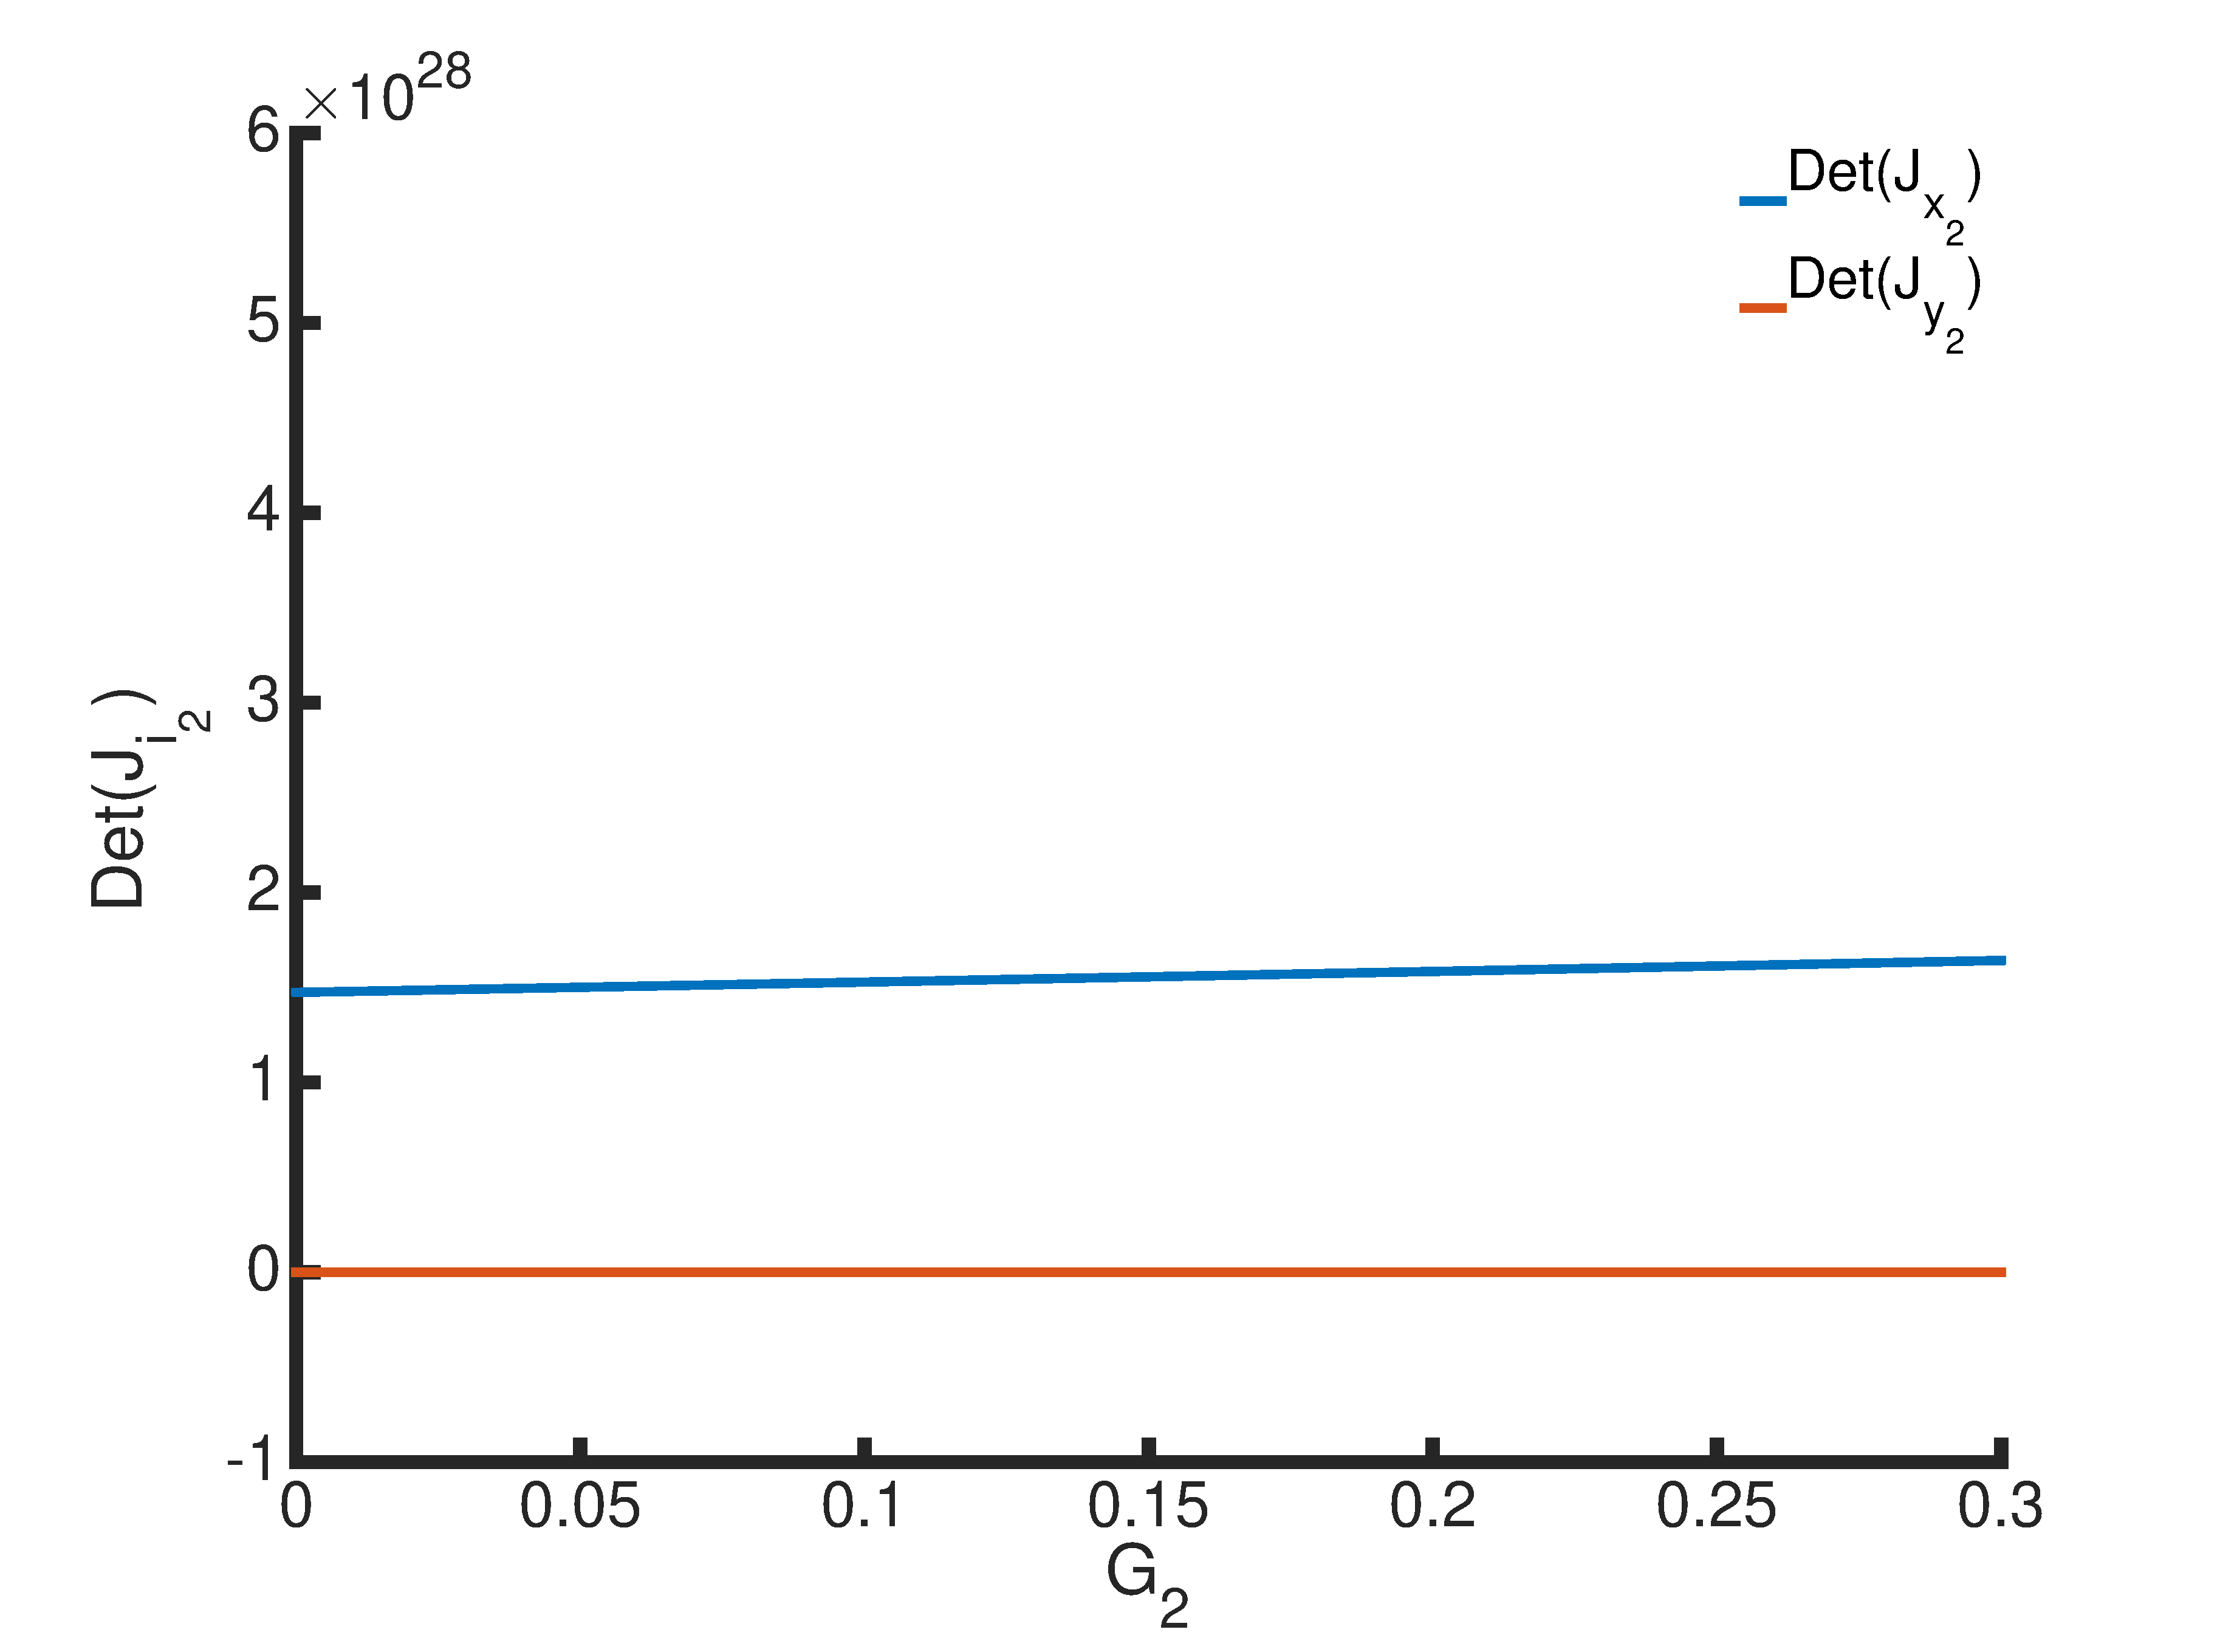
\includegraphics[width=\linewidth]{Figure1.eps}
                \label{fig:det_G2}
        \end{subfigure}
       \begin{subfigure}{0.49\textwidth}
       			\caption{\qquad}
                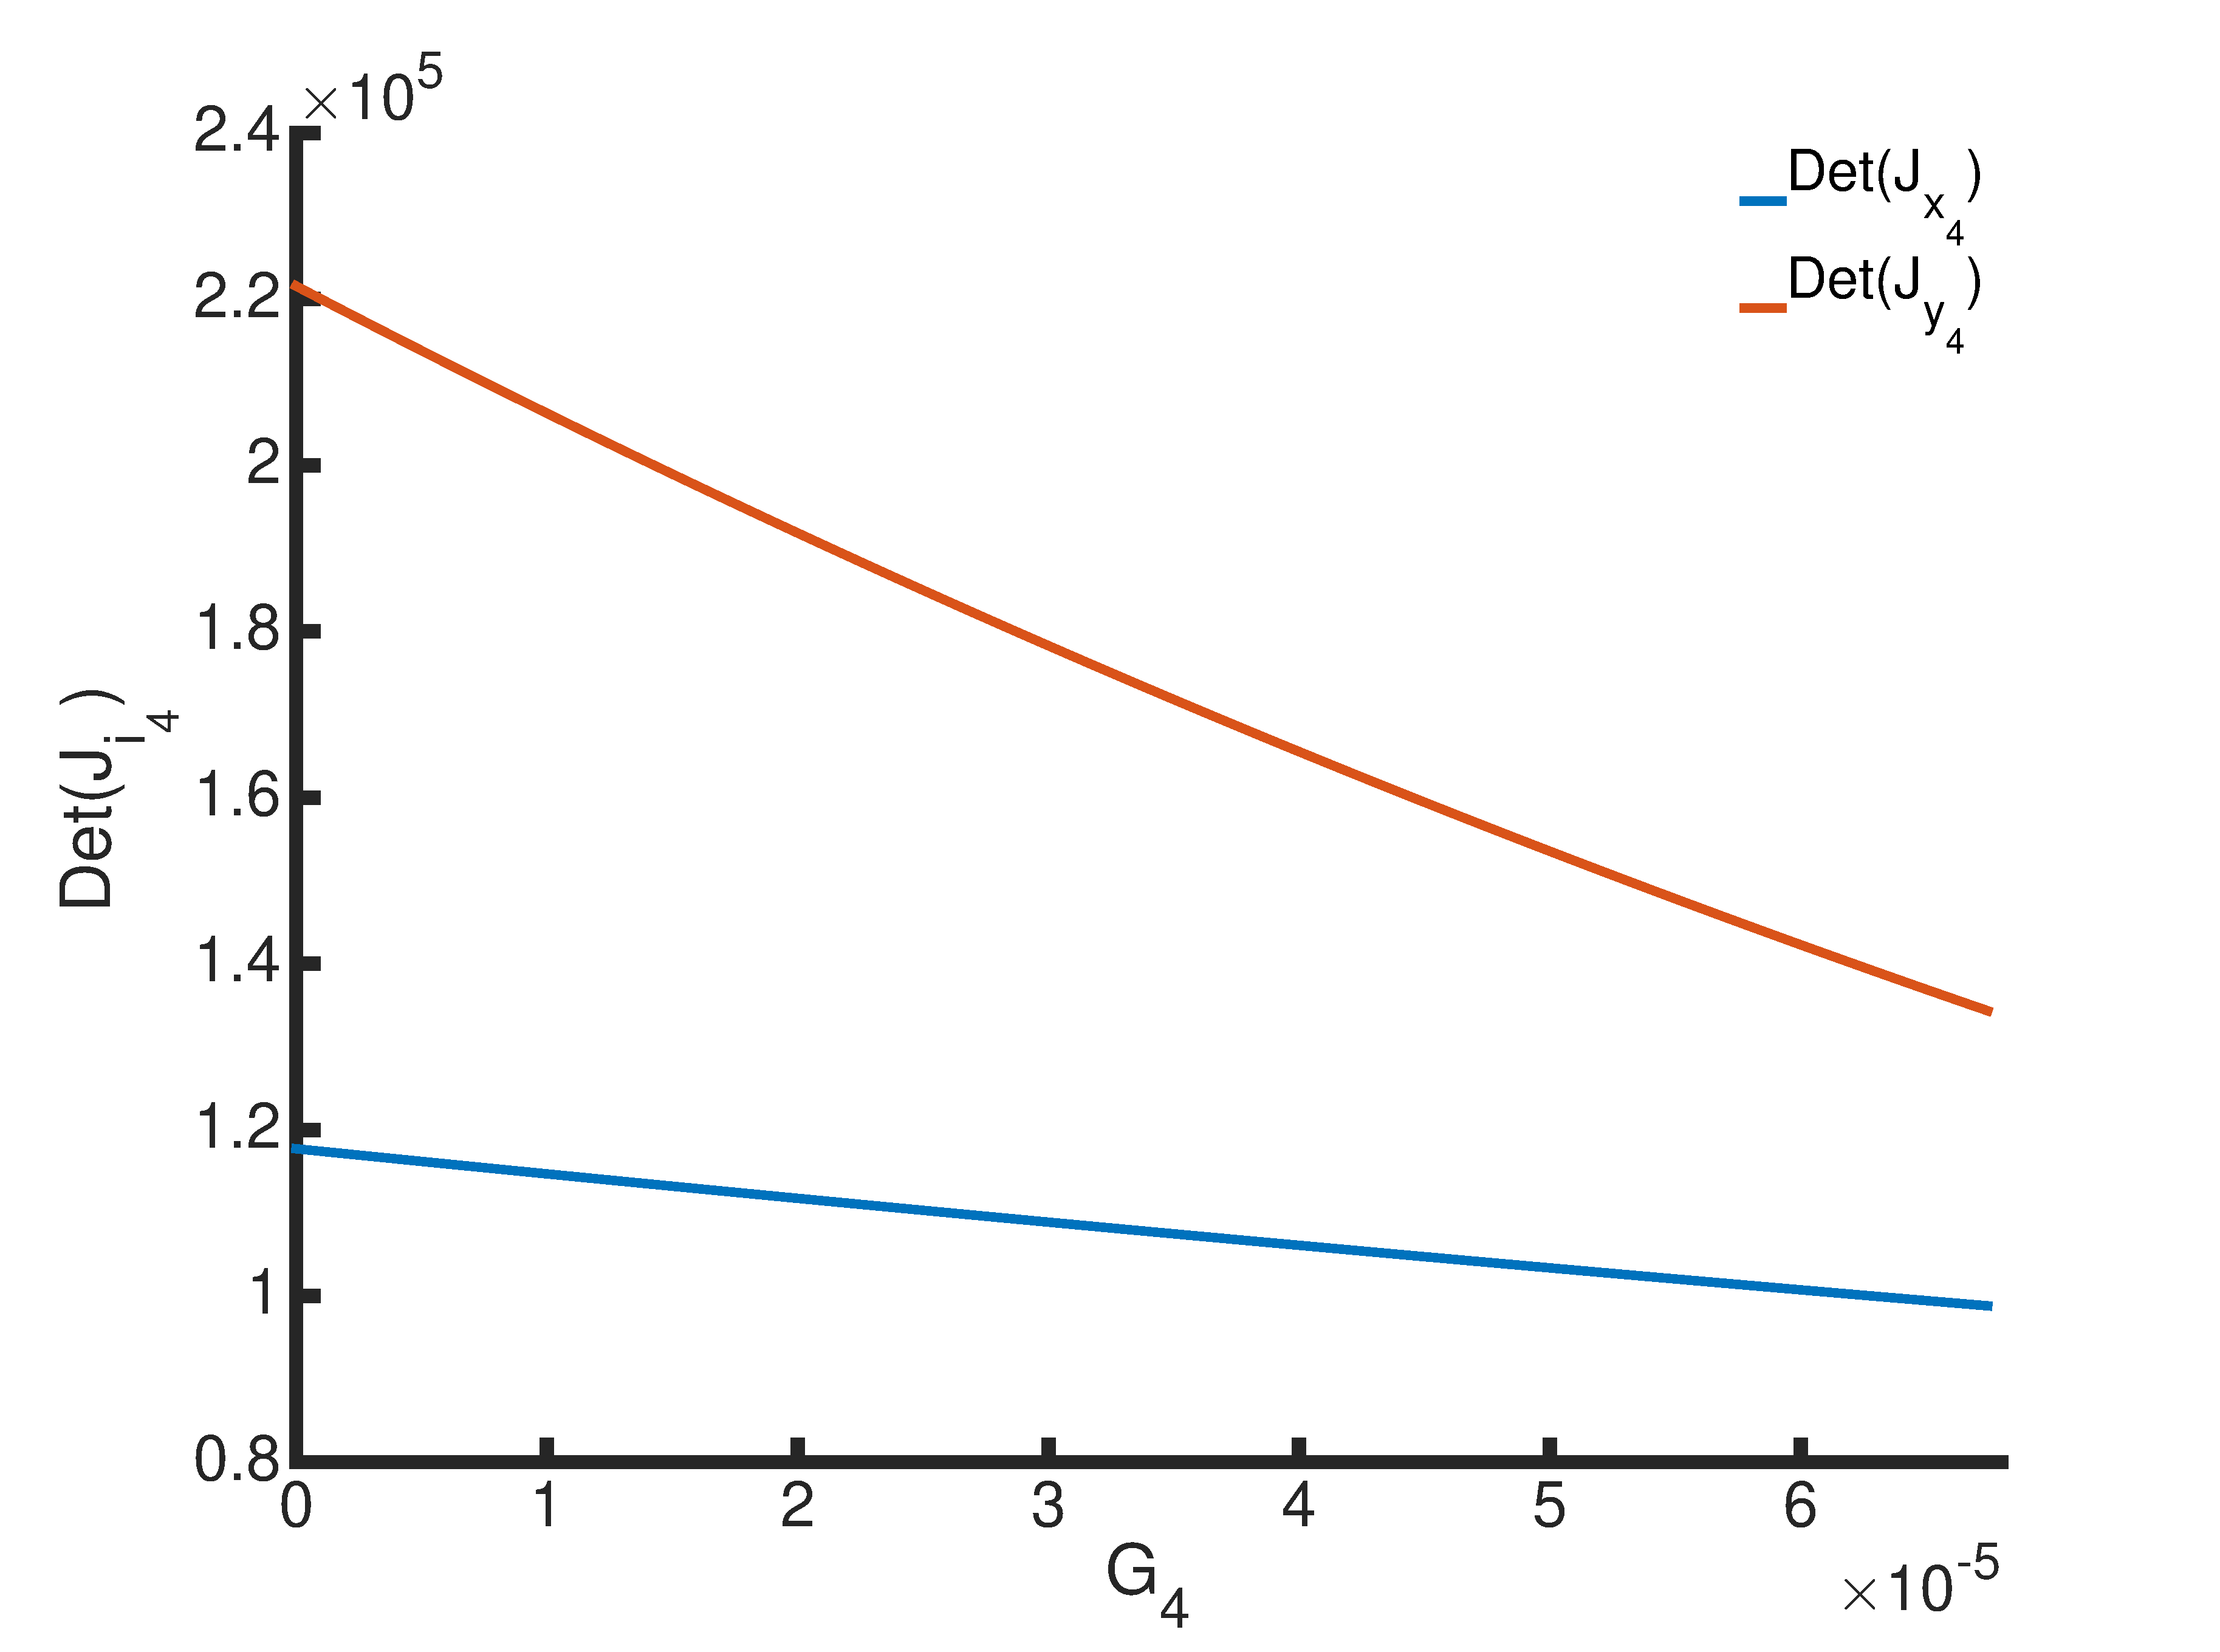
\includegraphics[width=\linewidth]{Figure2.eps}
                \label{fig:det_G4}
        \end{subfigure}     
		           
        
        \begin{subfigure}{0.49\textwidth}
				\caption{\qquad}                
                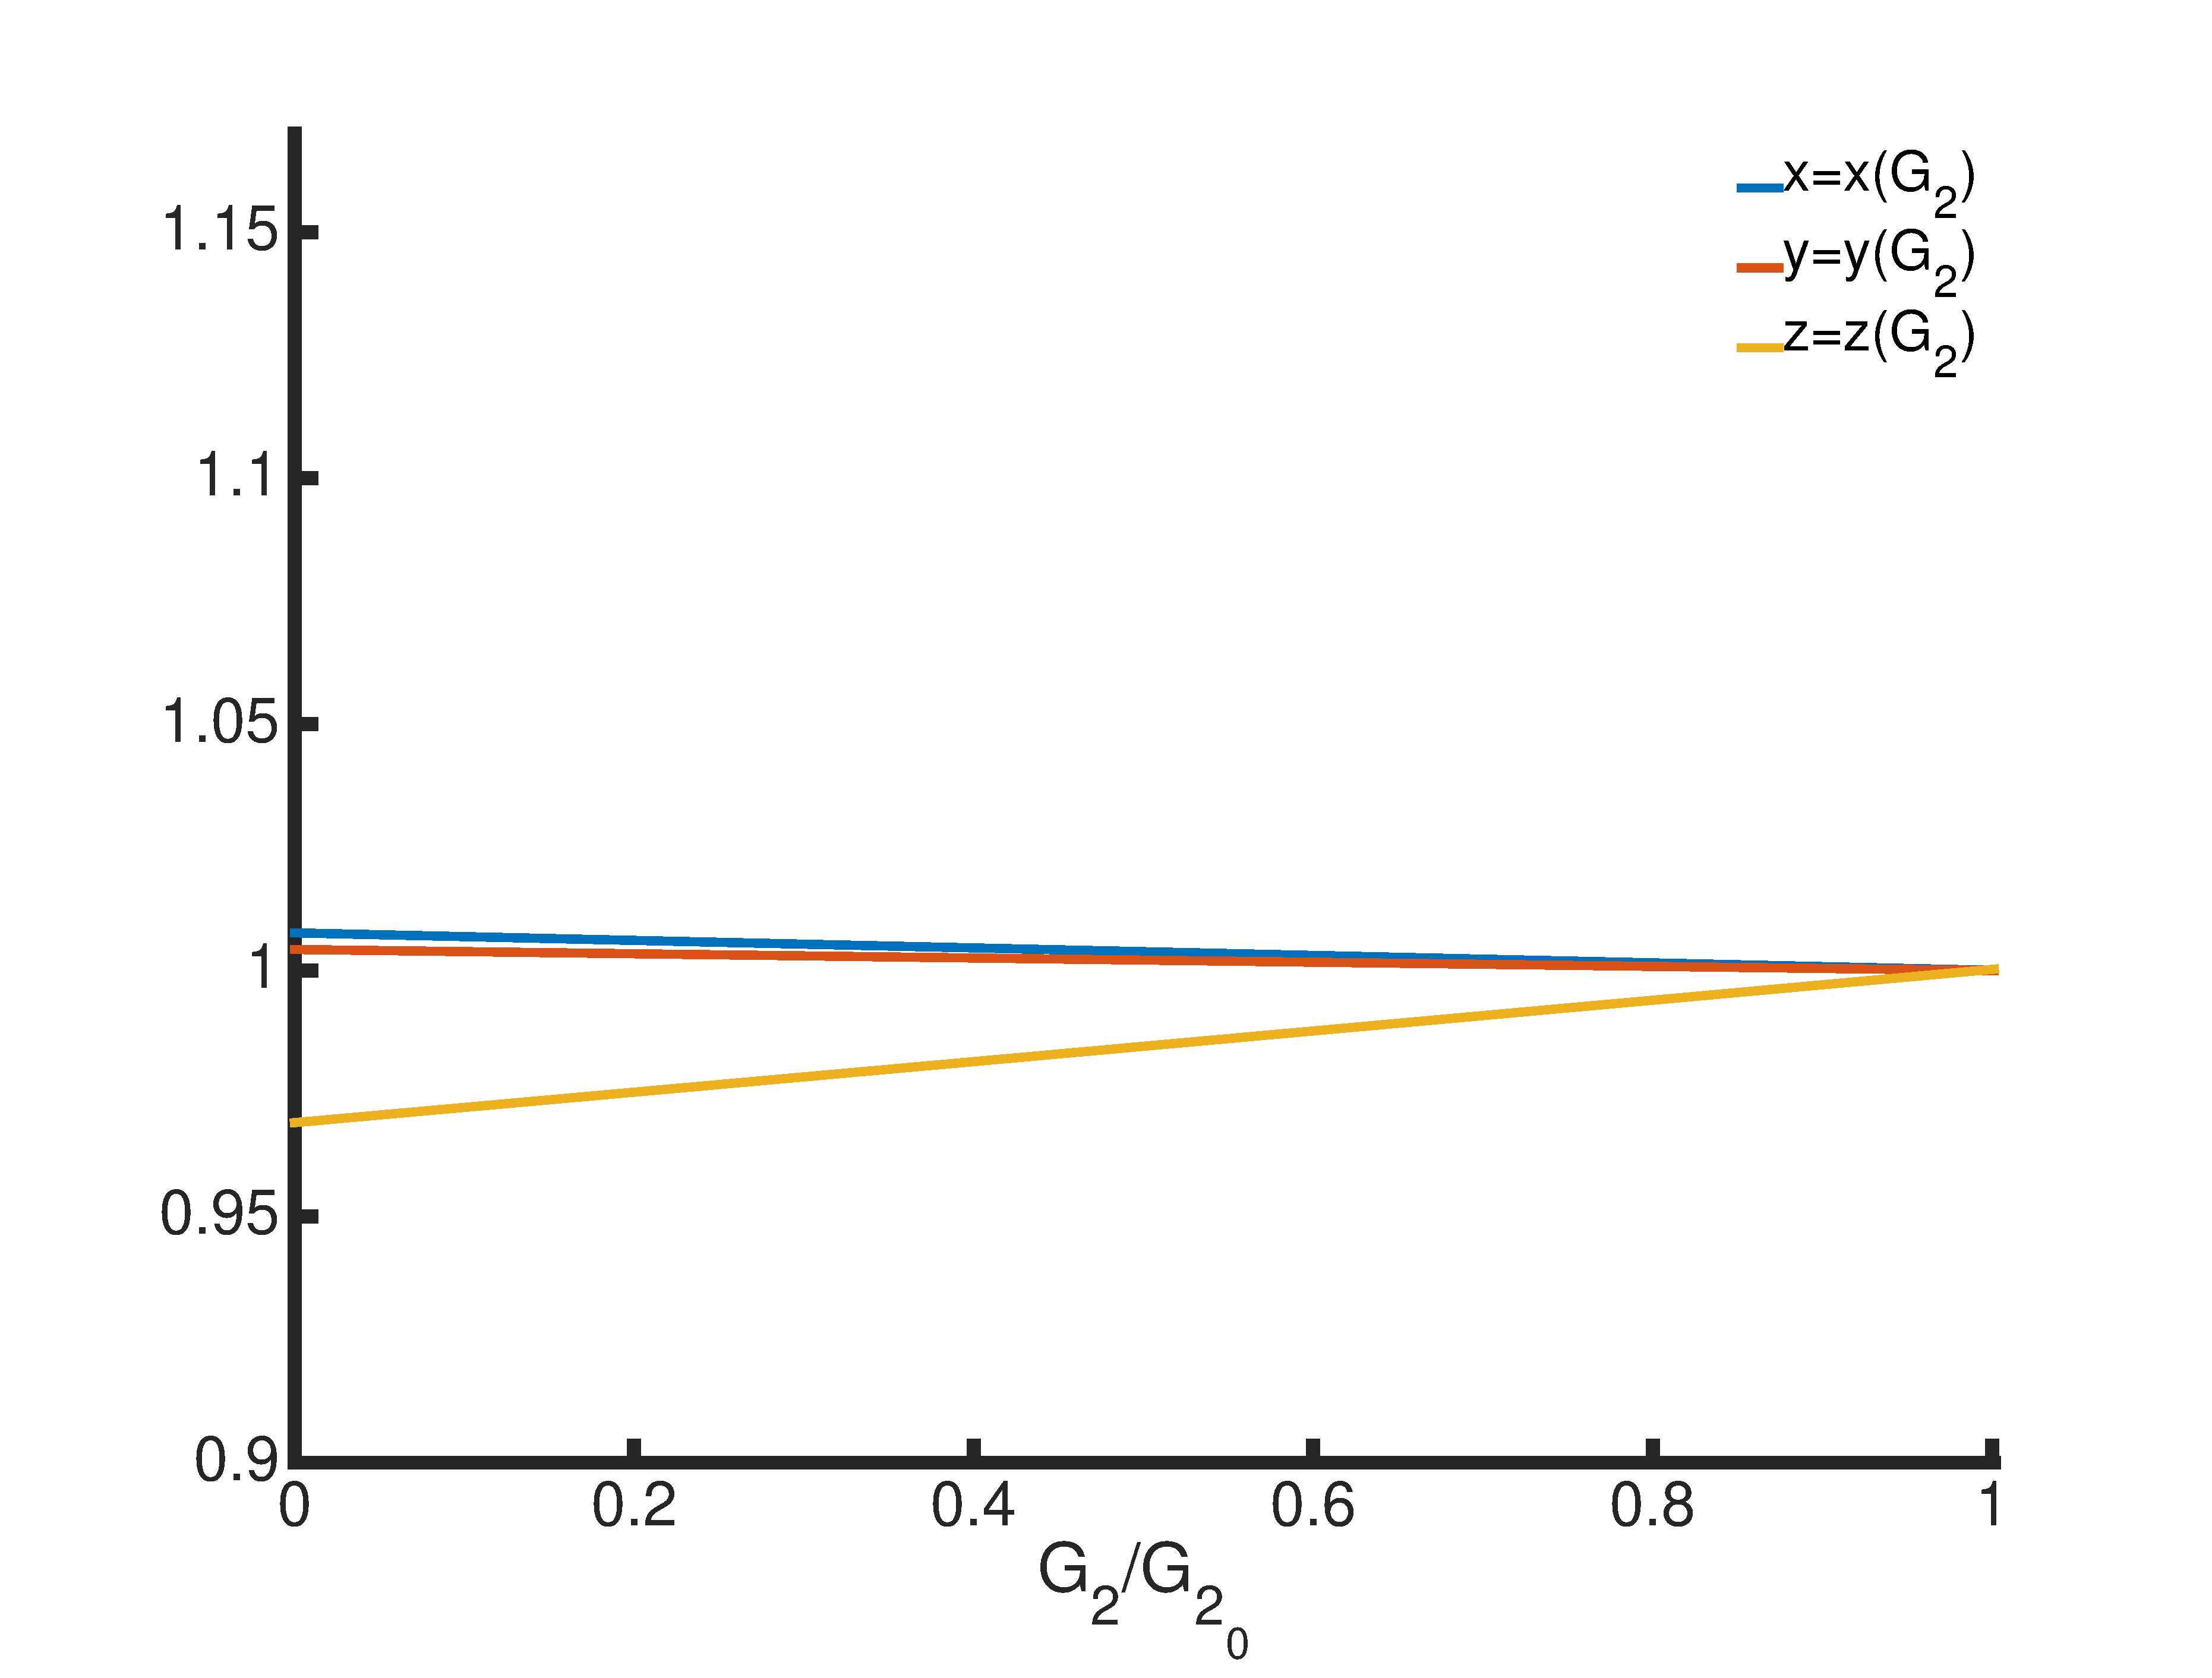
\includegraphics[width=\linewidth]{Figure5.eps}
                \label{fig:xyzG2}
        \end{subfigure}
       \begin{subfigure}{0.49\textwidth}
       			\caption{\qquad}
                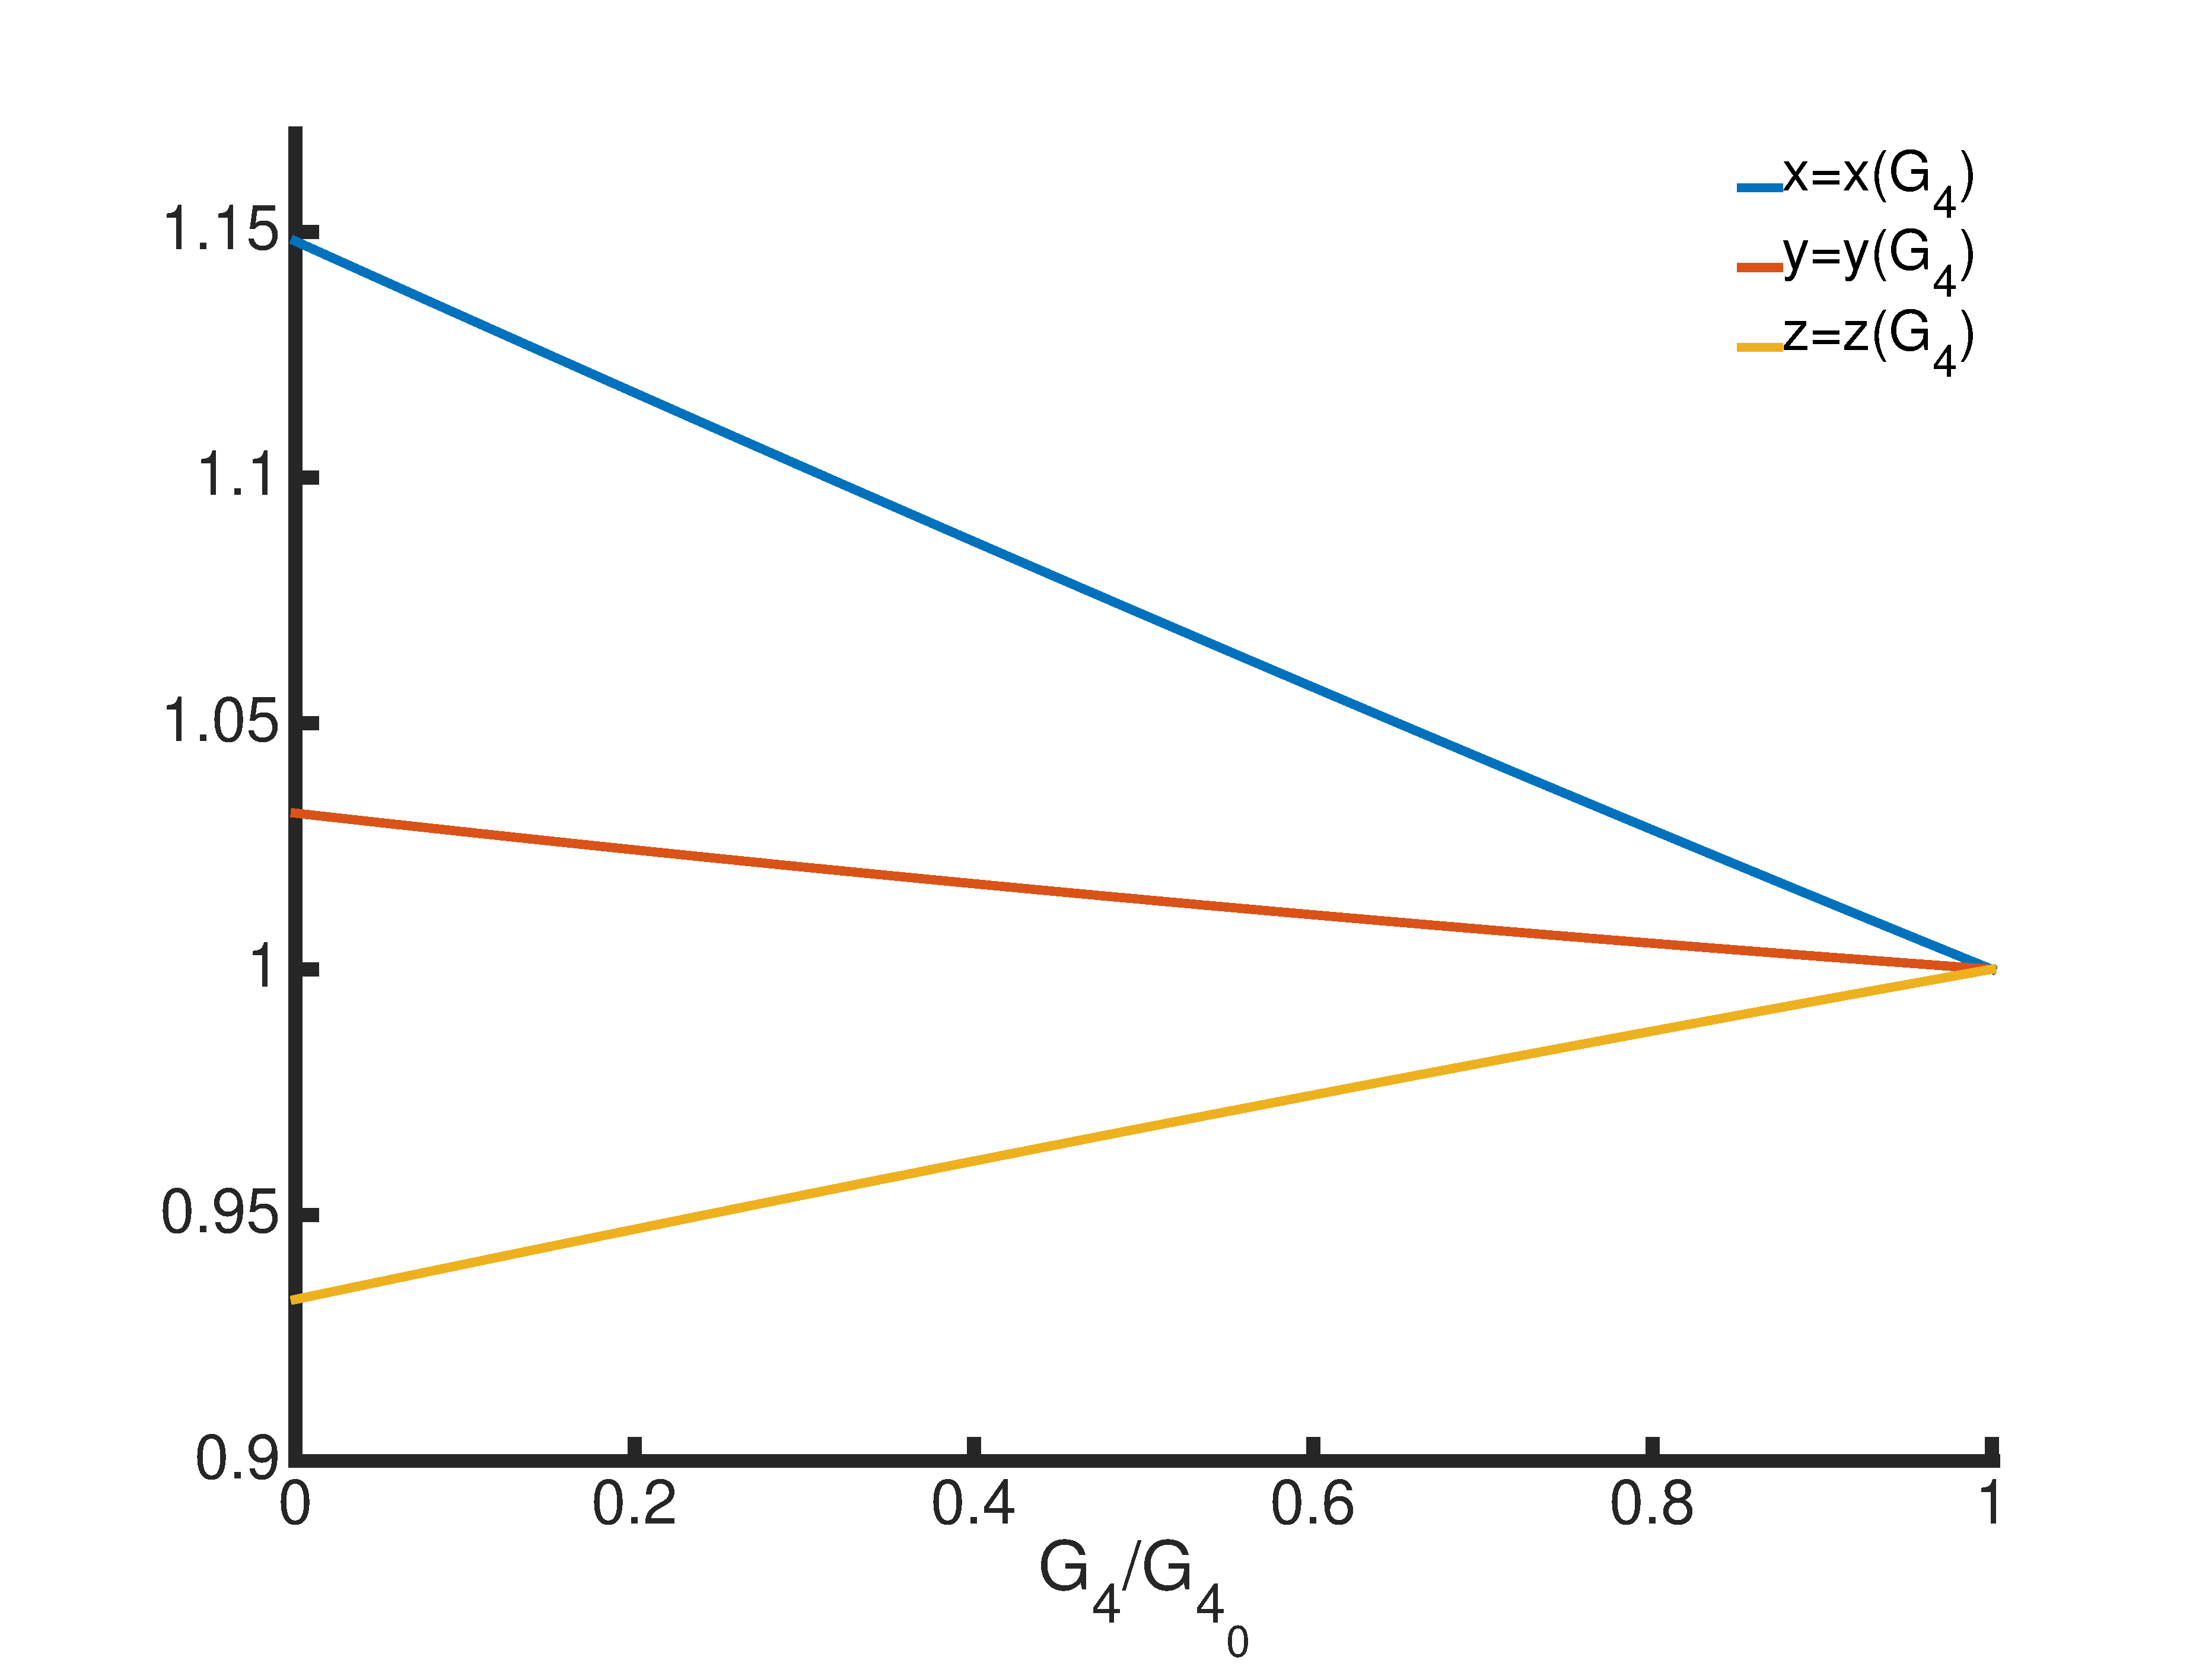
\includegraphics[width=\linewidth]{Figure4.eps}
                \label{fig:xyzG4}
        \end{subfigure}     
        
        \begin{subfigure}{0.49\textwidth}
        			\caption{\qquad}
                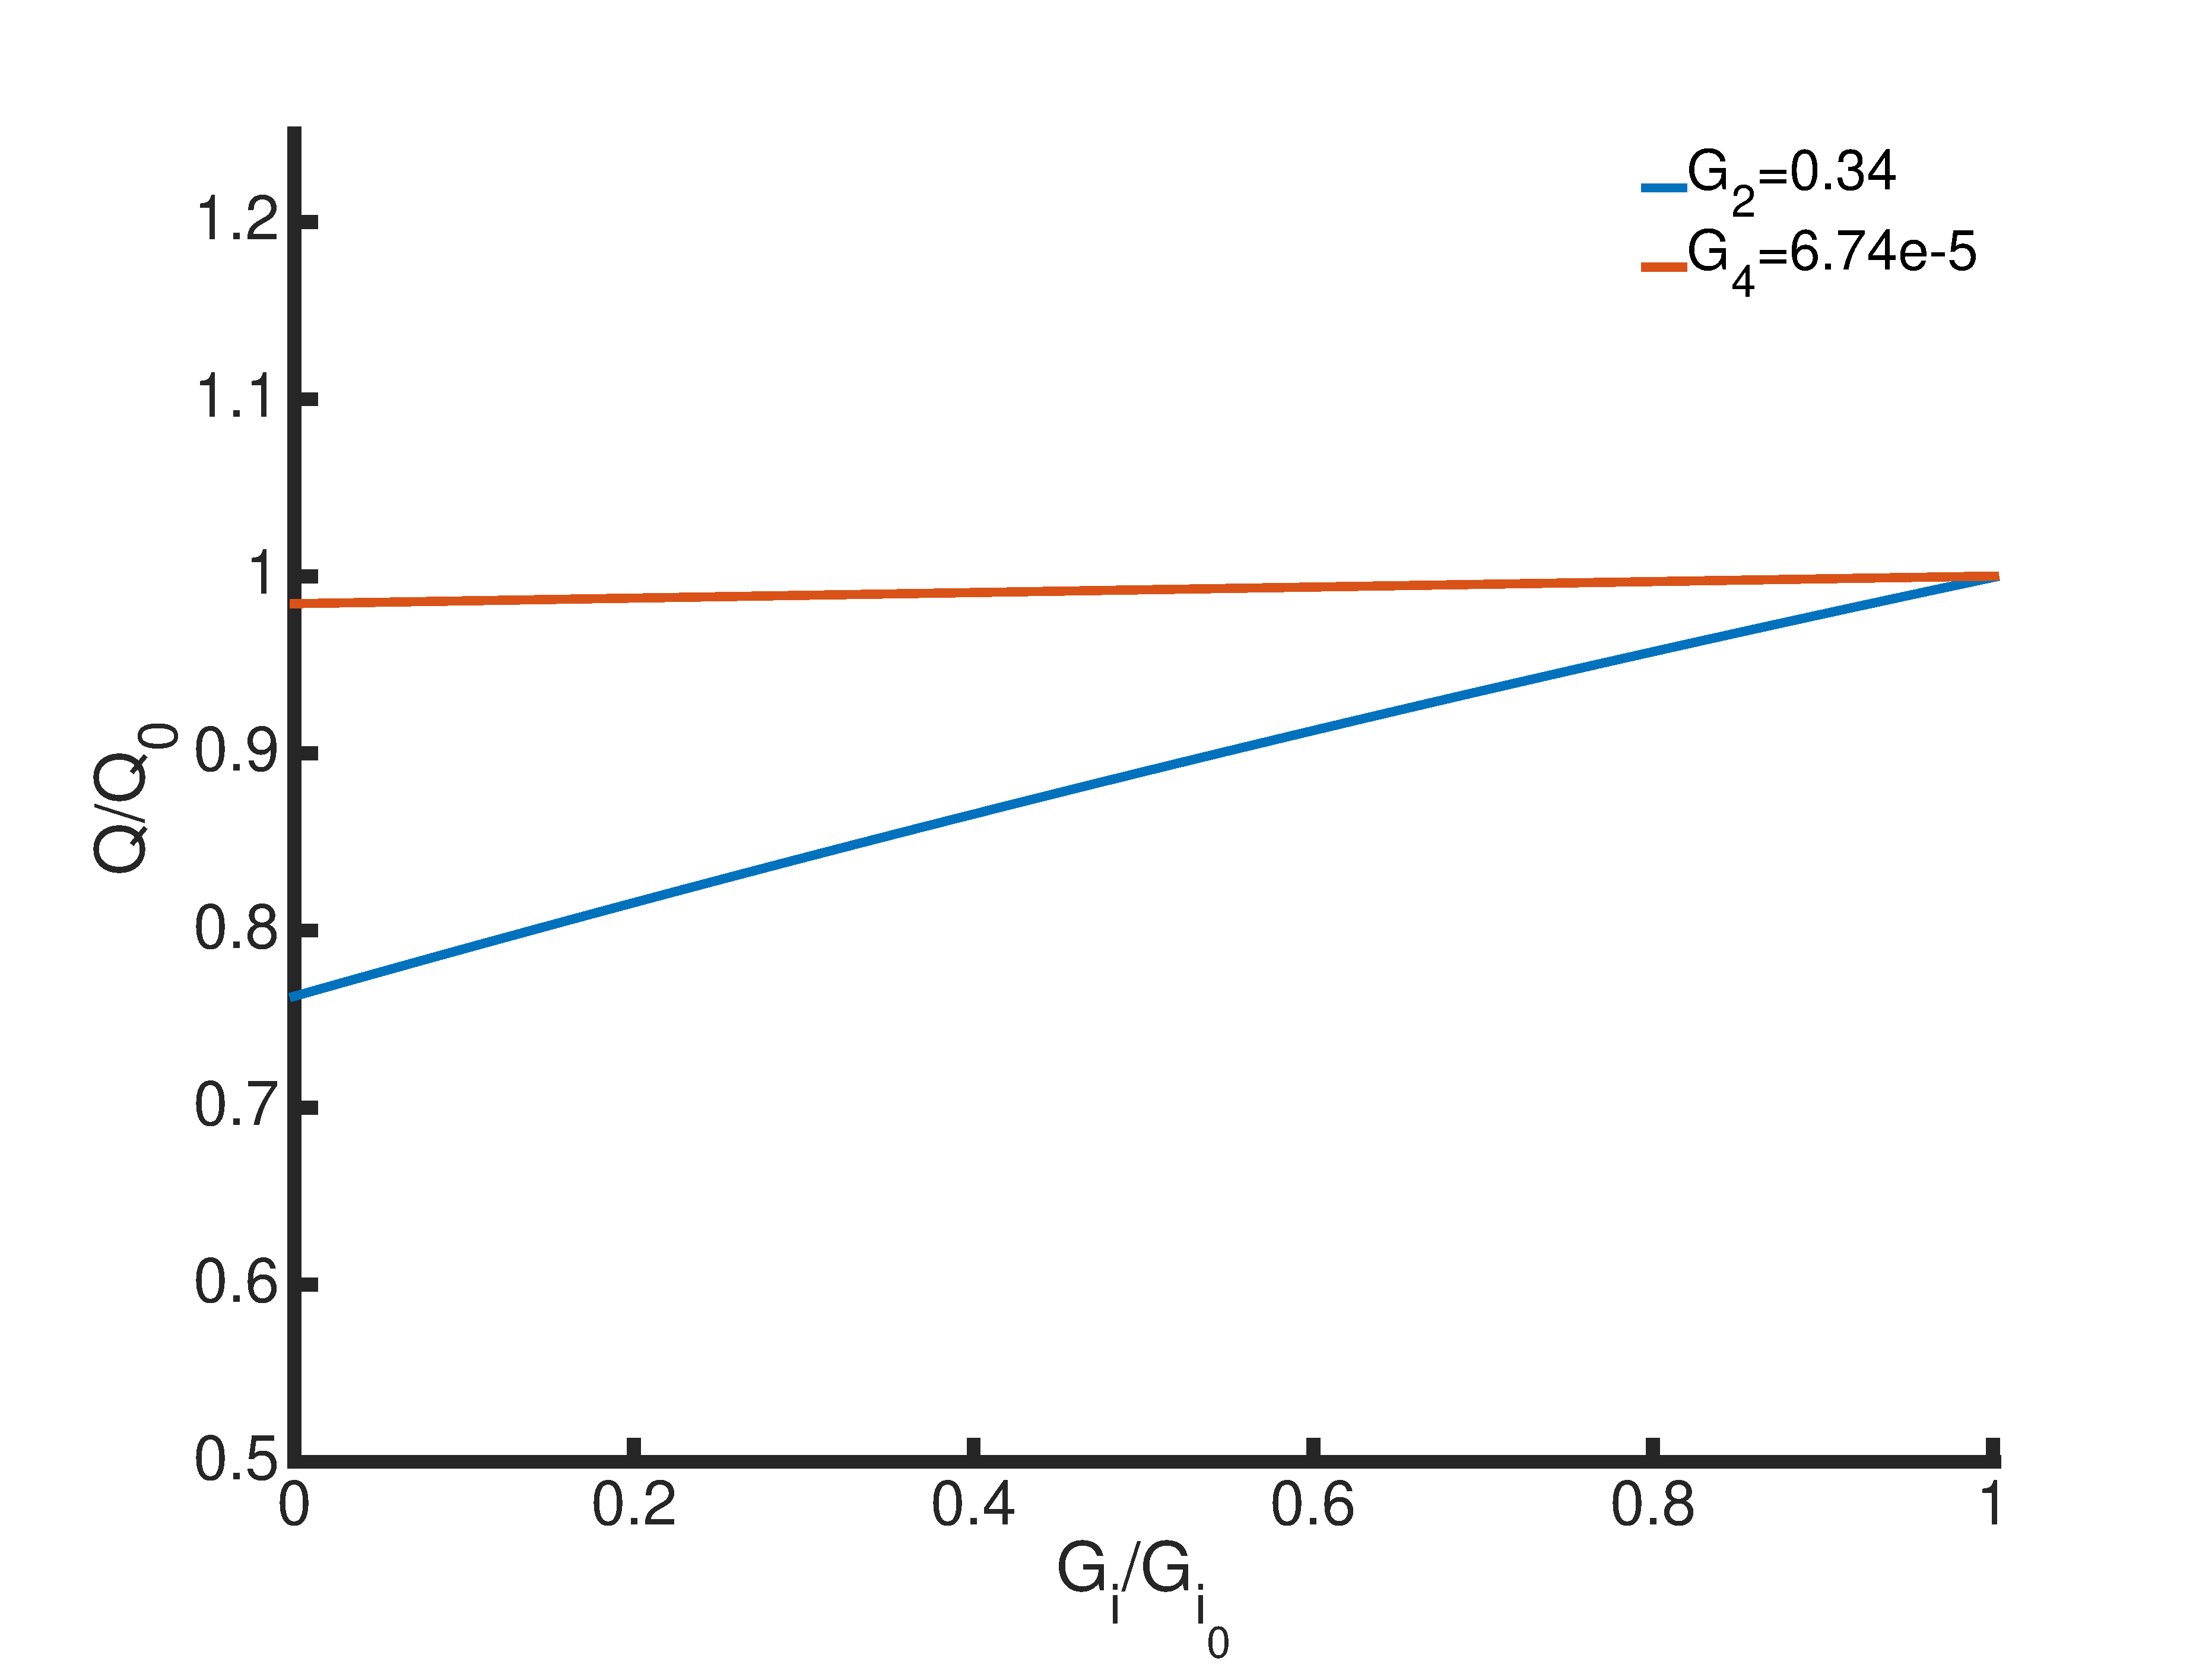
\includegraphics[width=\linewidth]{Figure3.eps}
                \label{fig:Q}
        \end{subfigure}
       \begin{subfigure}{0.49\textwidth}
       			\caption{\qquad}
                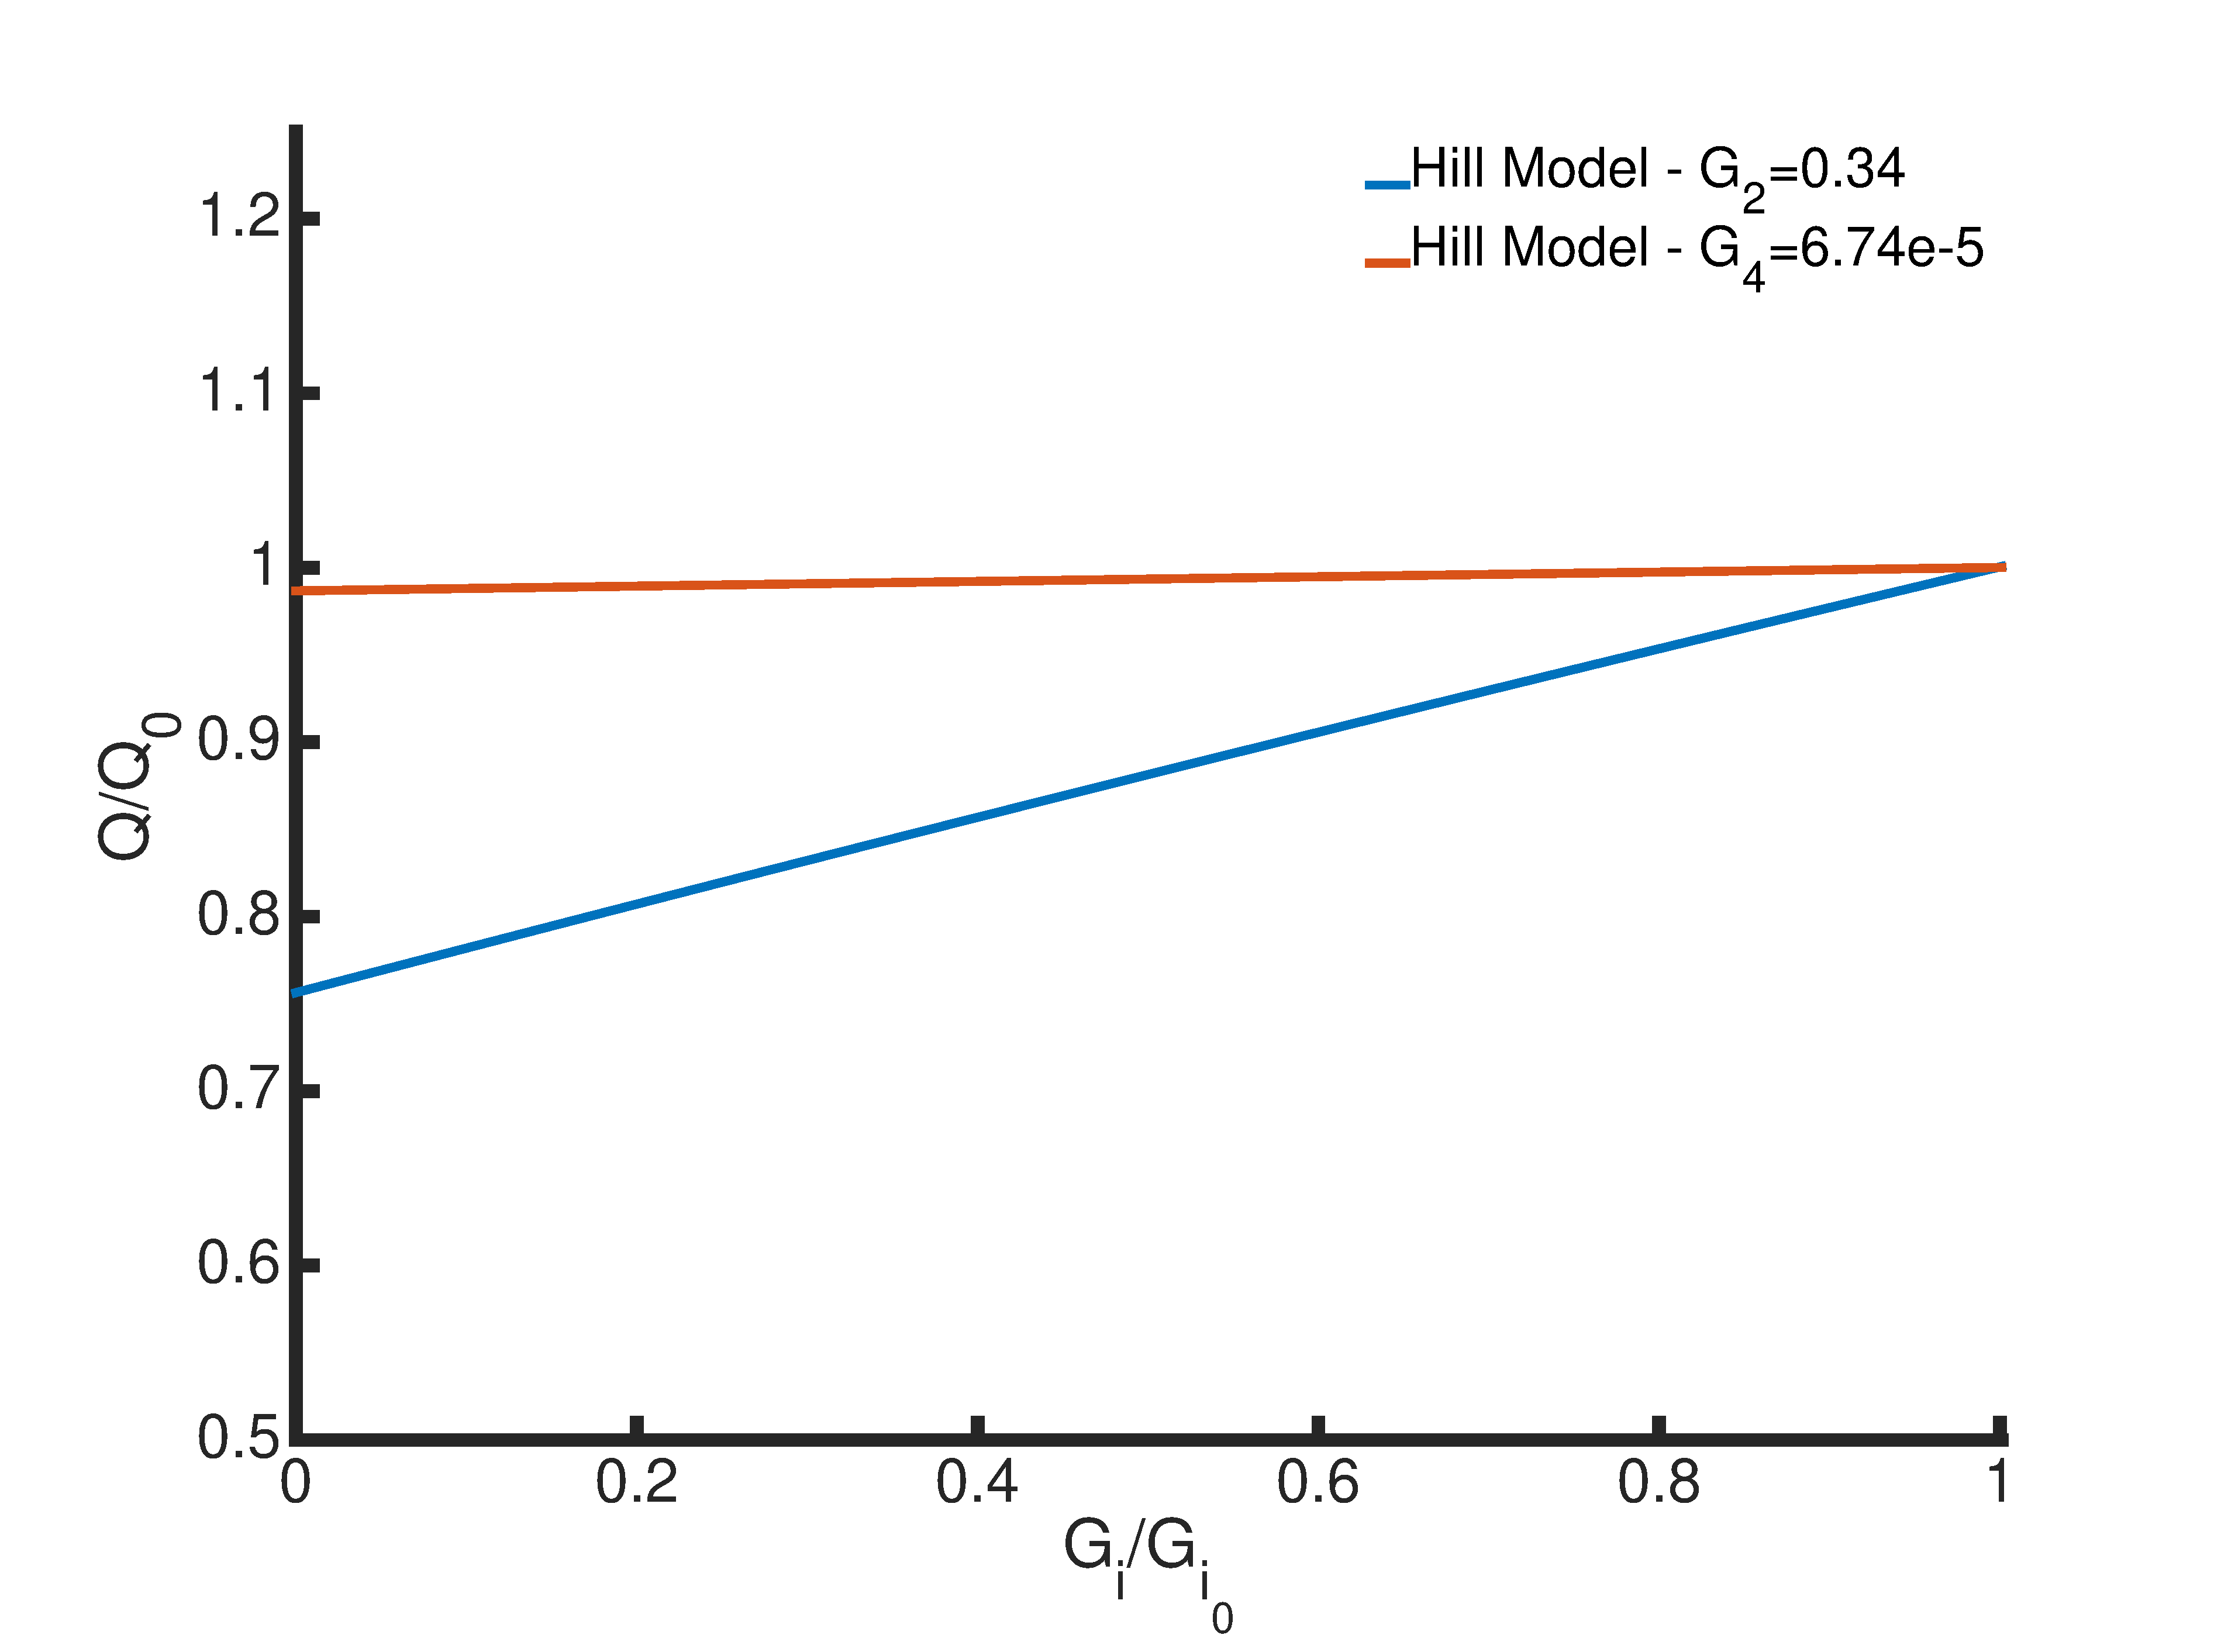
\includegraphics[width=\linewidth]{Figure6.eps}
                \label{fig:QH}
        \end{subfigure}  
        \caption{\textbf{A.} Determinant of the Jacobian matrix of the system as a function of the parameter $G_2$. \textbf{B.} Determinant of the Jacobian matrix of the system as a function of the parameter $G_4$. \textbf{C.} Set of steady state values of the variables of the system as a function of $G_2$. \textbf{D.} Set of steady state values of the variables of the system as a function of $G_4$. \textbf{E.} Fluid flow steady states as a function of the parameter $G_i$; where $i=2$ or $i=4$. \textbf{F.} Fluid flow steady states as a function of the parameter $G_i$; where $i=2$ or $i=4$, this time with a Hill function-type model. }
        \label{fig:results}      
\end{figure}
%%%%%%%%%%%%%%%%%%%%%%%%%%%%%%%%%%%%%%%%%%%%%%%%%%%%%%%%%%%%%%%%%%%%%%%%%%%%%%%%%%%%%%%%%%%%%%%%
%%%%%%%%%%%%%%%%%%%%%%%%%%%%%%%%%%%%%%%%%%%%%%%%%%%%%%%%%%%%%%%%%%%%%%%%%%%%%%%%%%%%%%%%%%%%%%%%
%%%%%%%%%%%%%%%%%%%%%%%%%%%%%%%%%%%%%%%%%%%%%%%%%%%%%%%%%%%%%%%%%%%%%%%%%%%%%%%%%%%%%%%%%%%%%%%%

\subsection{\bf Sensitivity of the model to parameters}
%%%%%%%%%%%%%%%%%%%%%%%%%%%%%%%%%%%%%%%%%%%%%%%%%%%%%%%%%%%%%%%%%%%%%%%%%%%%%%%%%%%%%%%%%%%%%%%%
%%%%%%%%%%%%%%%%%%%%%%%%%%%%%%%%%%%%%%%%%%%%%%%%%%%%%%%%%%%%%%%%%%%%%%%%%%%%%%%%%%%%%%%%%%%%%%%%
%%%%%%%%%%%%%%%%%%%%%%%%%%%%%%%%%%%%%%%%%%%%%%%%%%%%%%%%%%%%%%%%%%%%%%%%%%%%%%%%%%%%%%%%%%%%%%%%
\begin{figure}
\centering
        \begin{subfigure}{0.49\textwidth}
        			\caption{\qquad}
                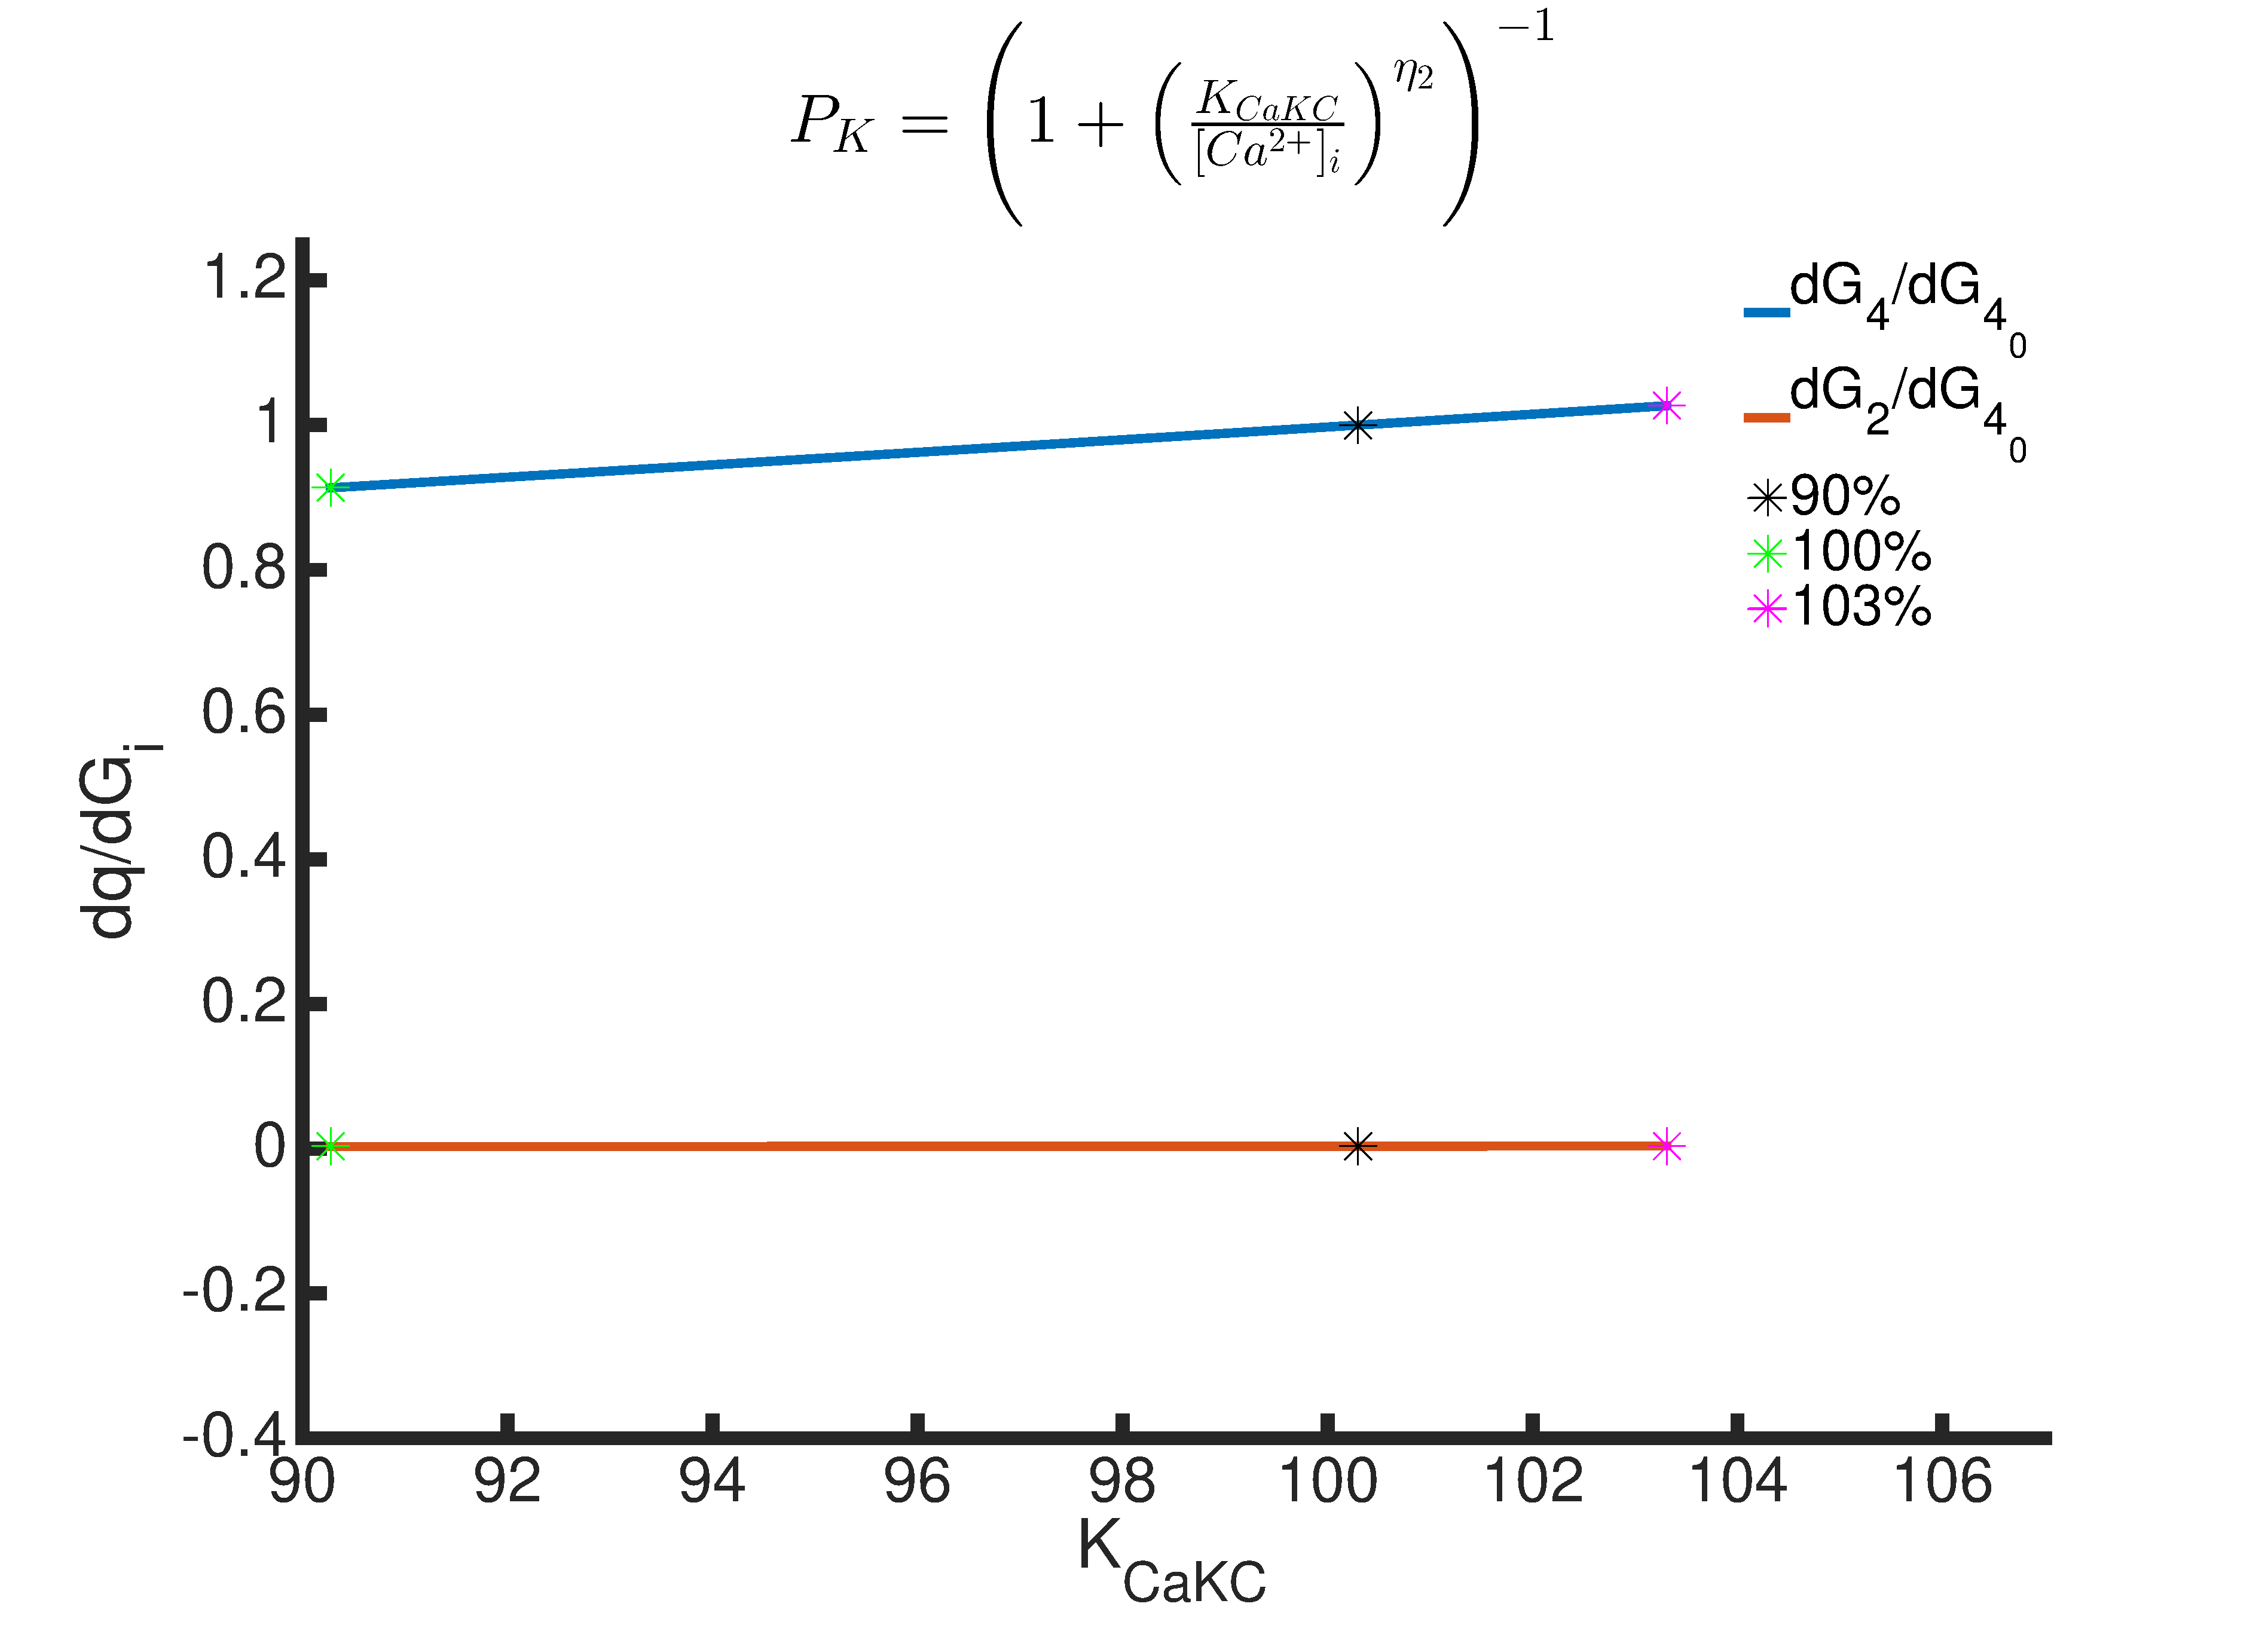
\includegraphics[width=\linewidth]{Figure7.eps}
                \label{fig:det_G2}
        \end{subfigure}
       \begin{subfigure}{0.49\textwidth}
       			\caption{\qquad}
                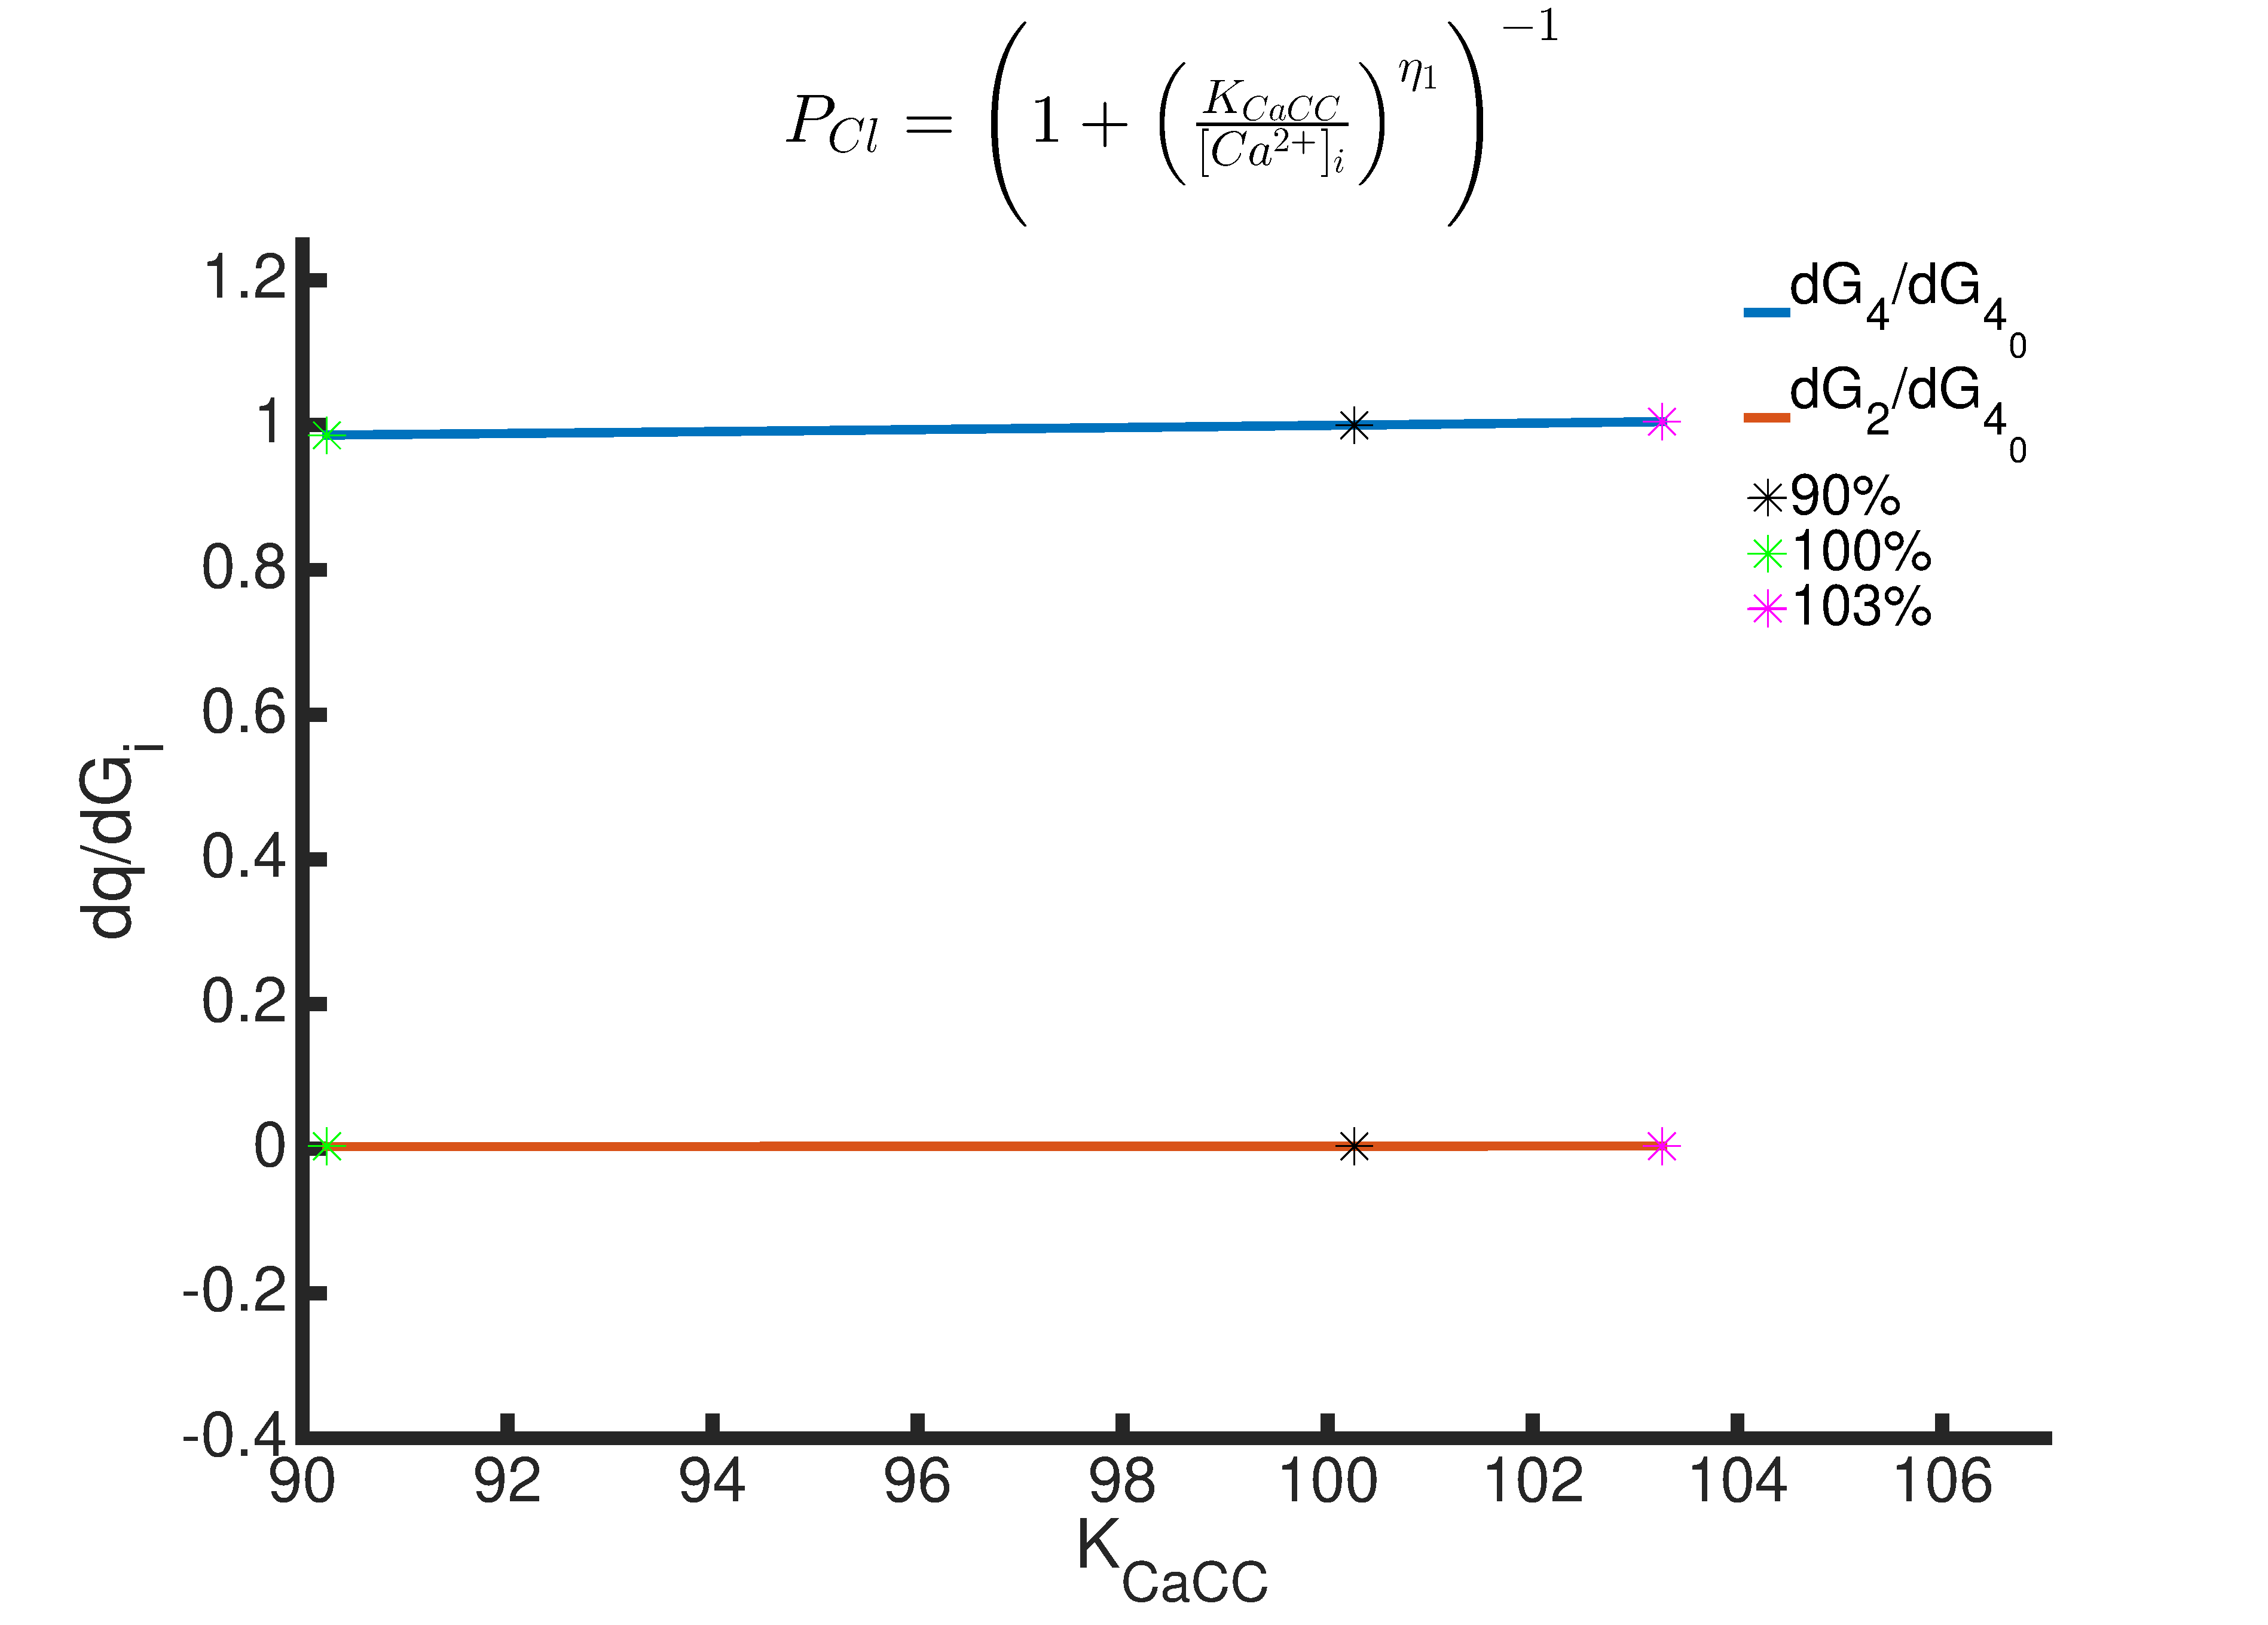
\includegraphics[width=\linewidth]{Figure20.eps}
                \label{fig:det_G4}
        \end{subfigure}     
		           
        
        \begin{subfigure}{0.49\textwidth}
        			\caption{\qquad}
                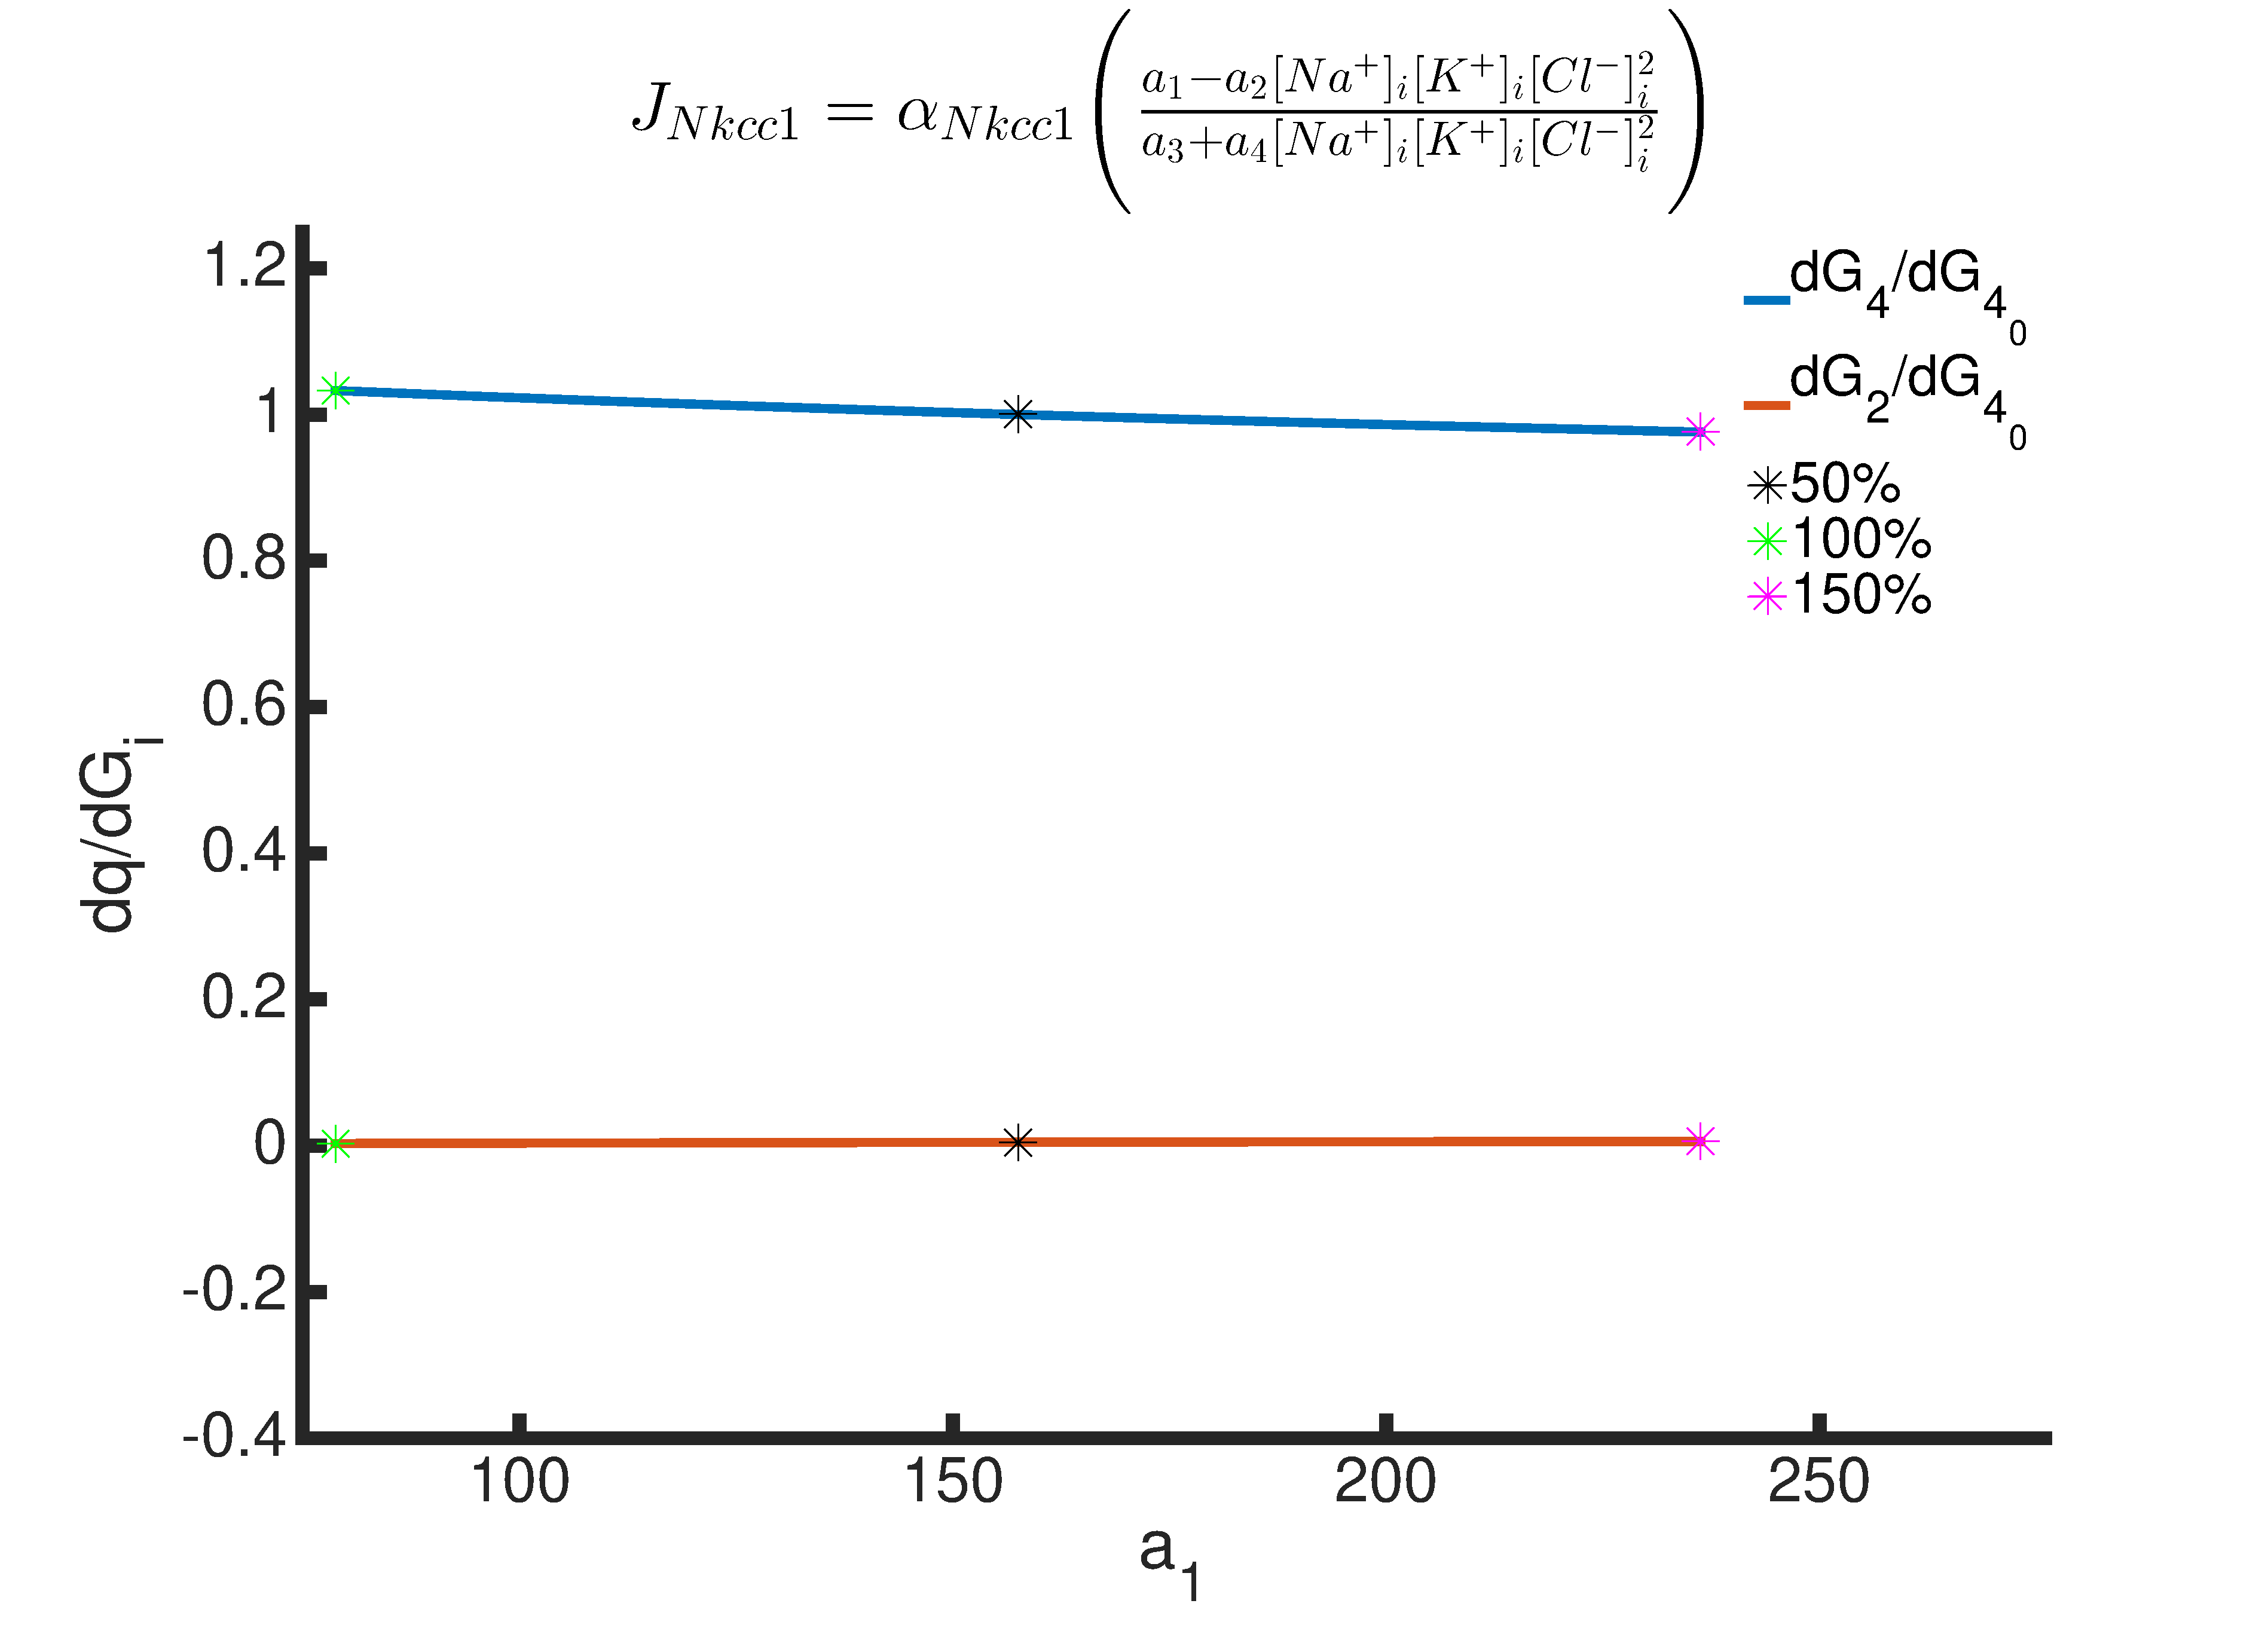
\includegraphics[width=\linewidth]{Figure14.eps}
                \label{fig:xyzG2}
        \end{subfigure}
       \begin{subfigure}{0.49\textwidth}
       			\caption{\qquad}
                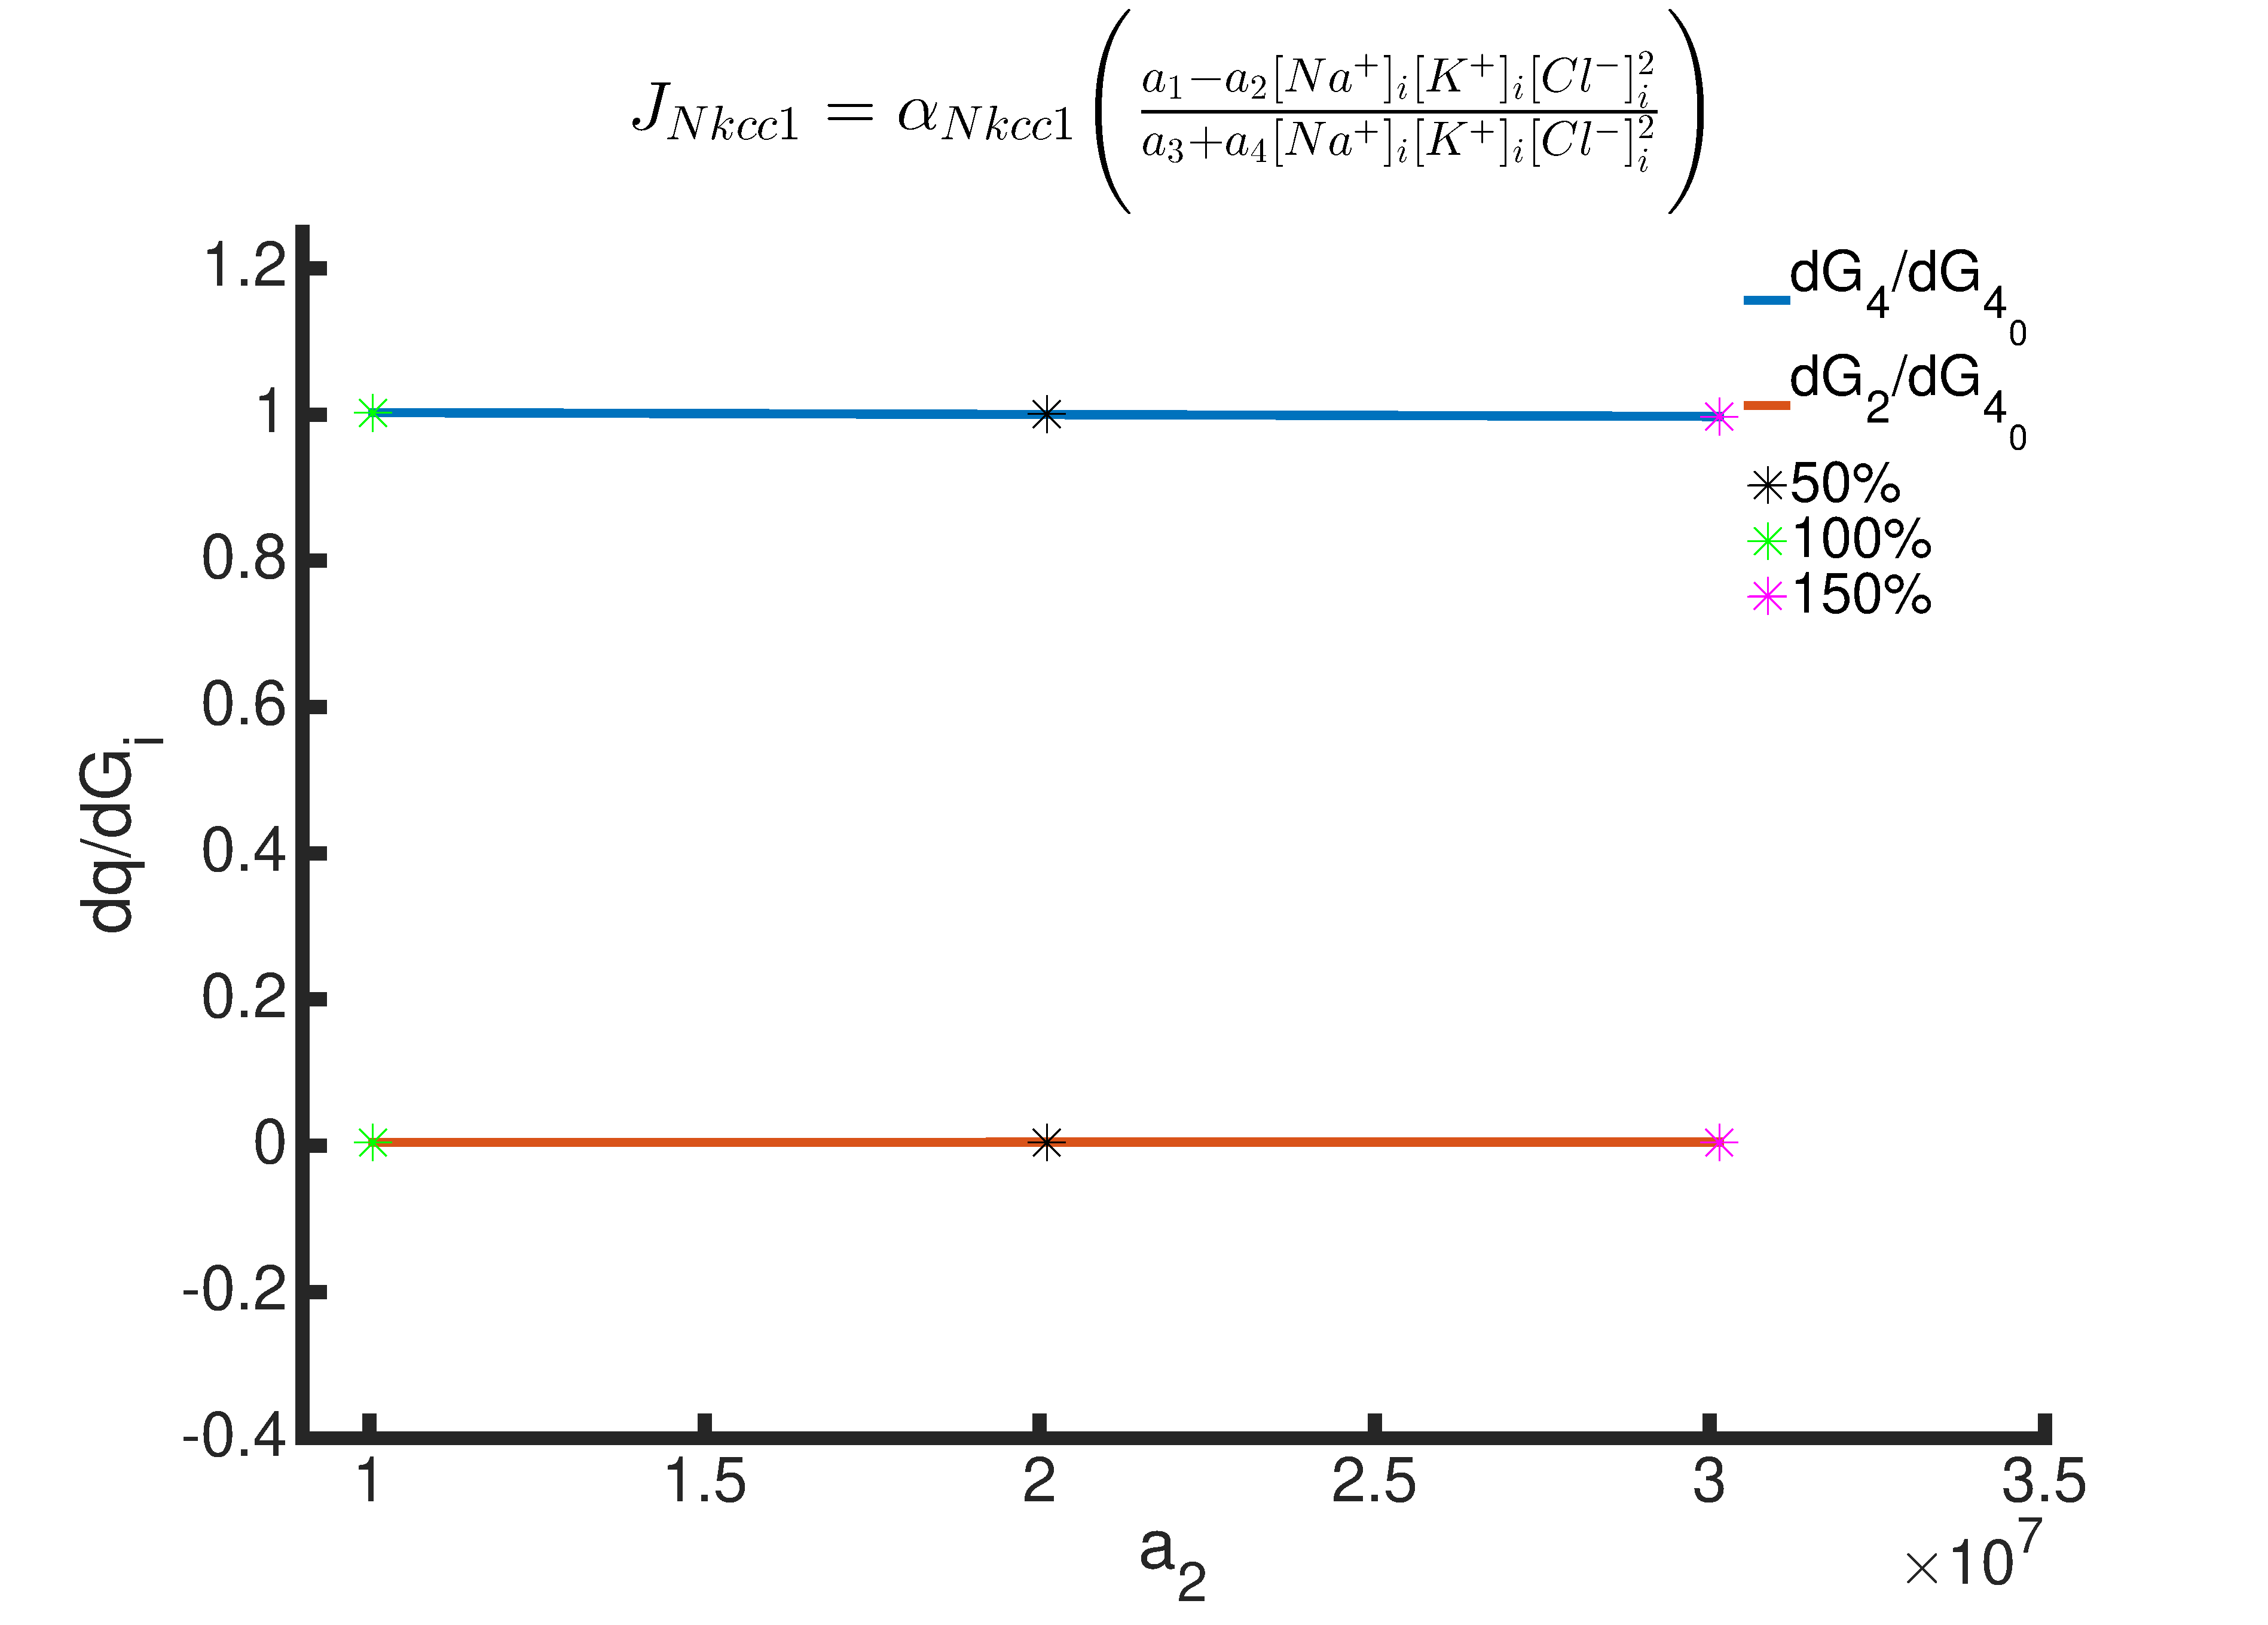
\includegraphics[width=\linewidth]{Figure15.eps}
                \label{fig:xyzG4}
        \end{subfigure}     
        
        \begin{subfigure}{0.49\textwidth}
       		    \caption{\qquad}
                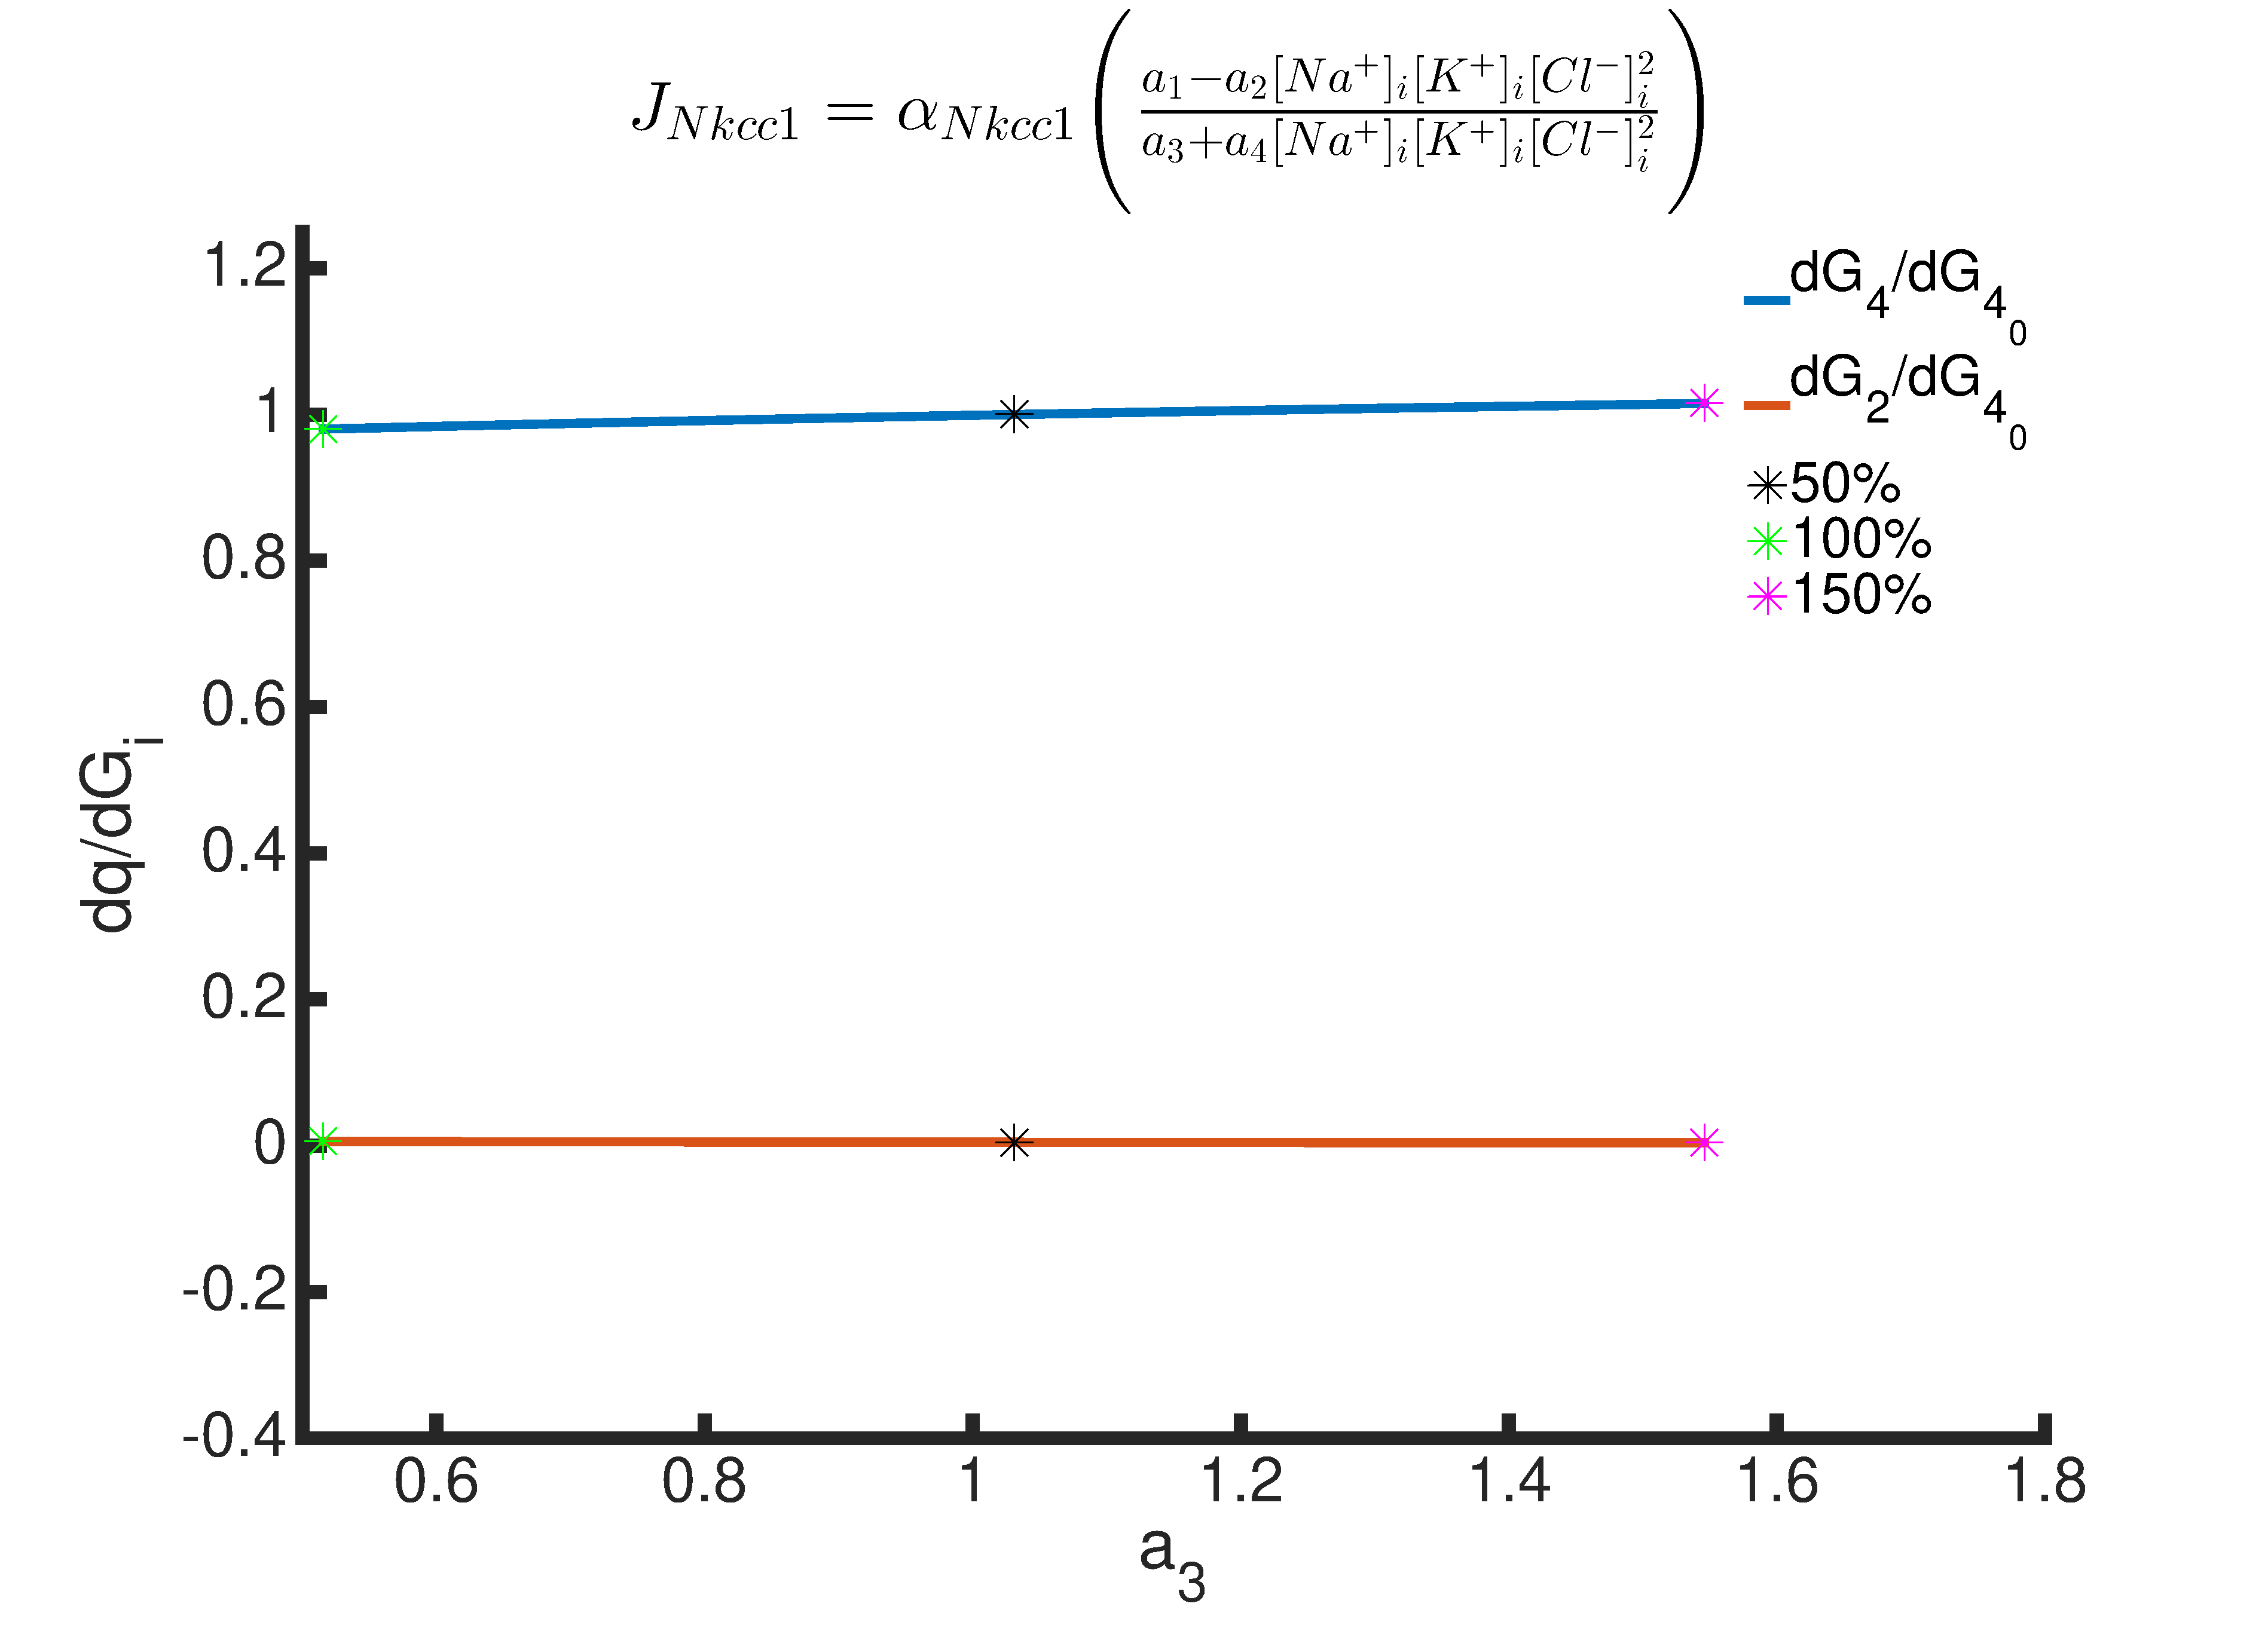
\includegraphics[width=\linewidth]{Figure16.eps}
                \label{fig:Q}
        \end{subfigure}
       \begin{subfigure}{0.49\textwidth}
       			\caption{\qquad}
                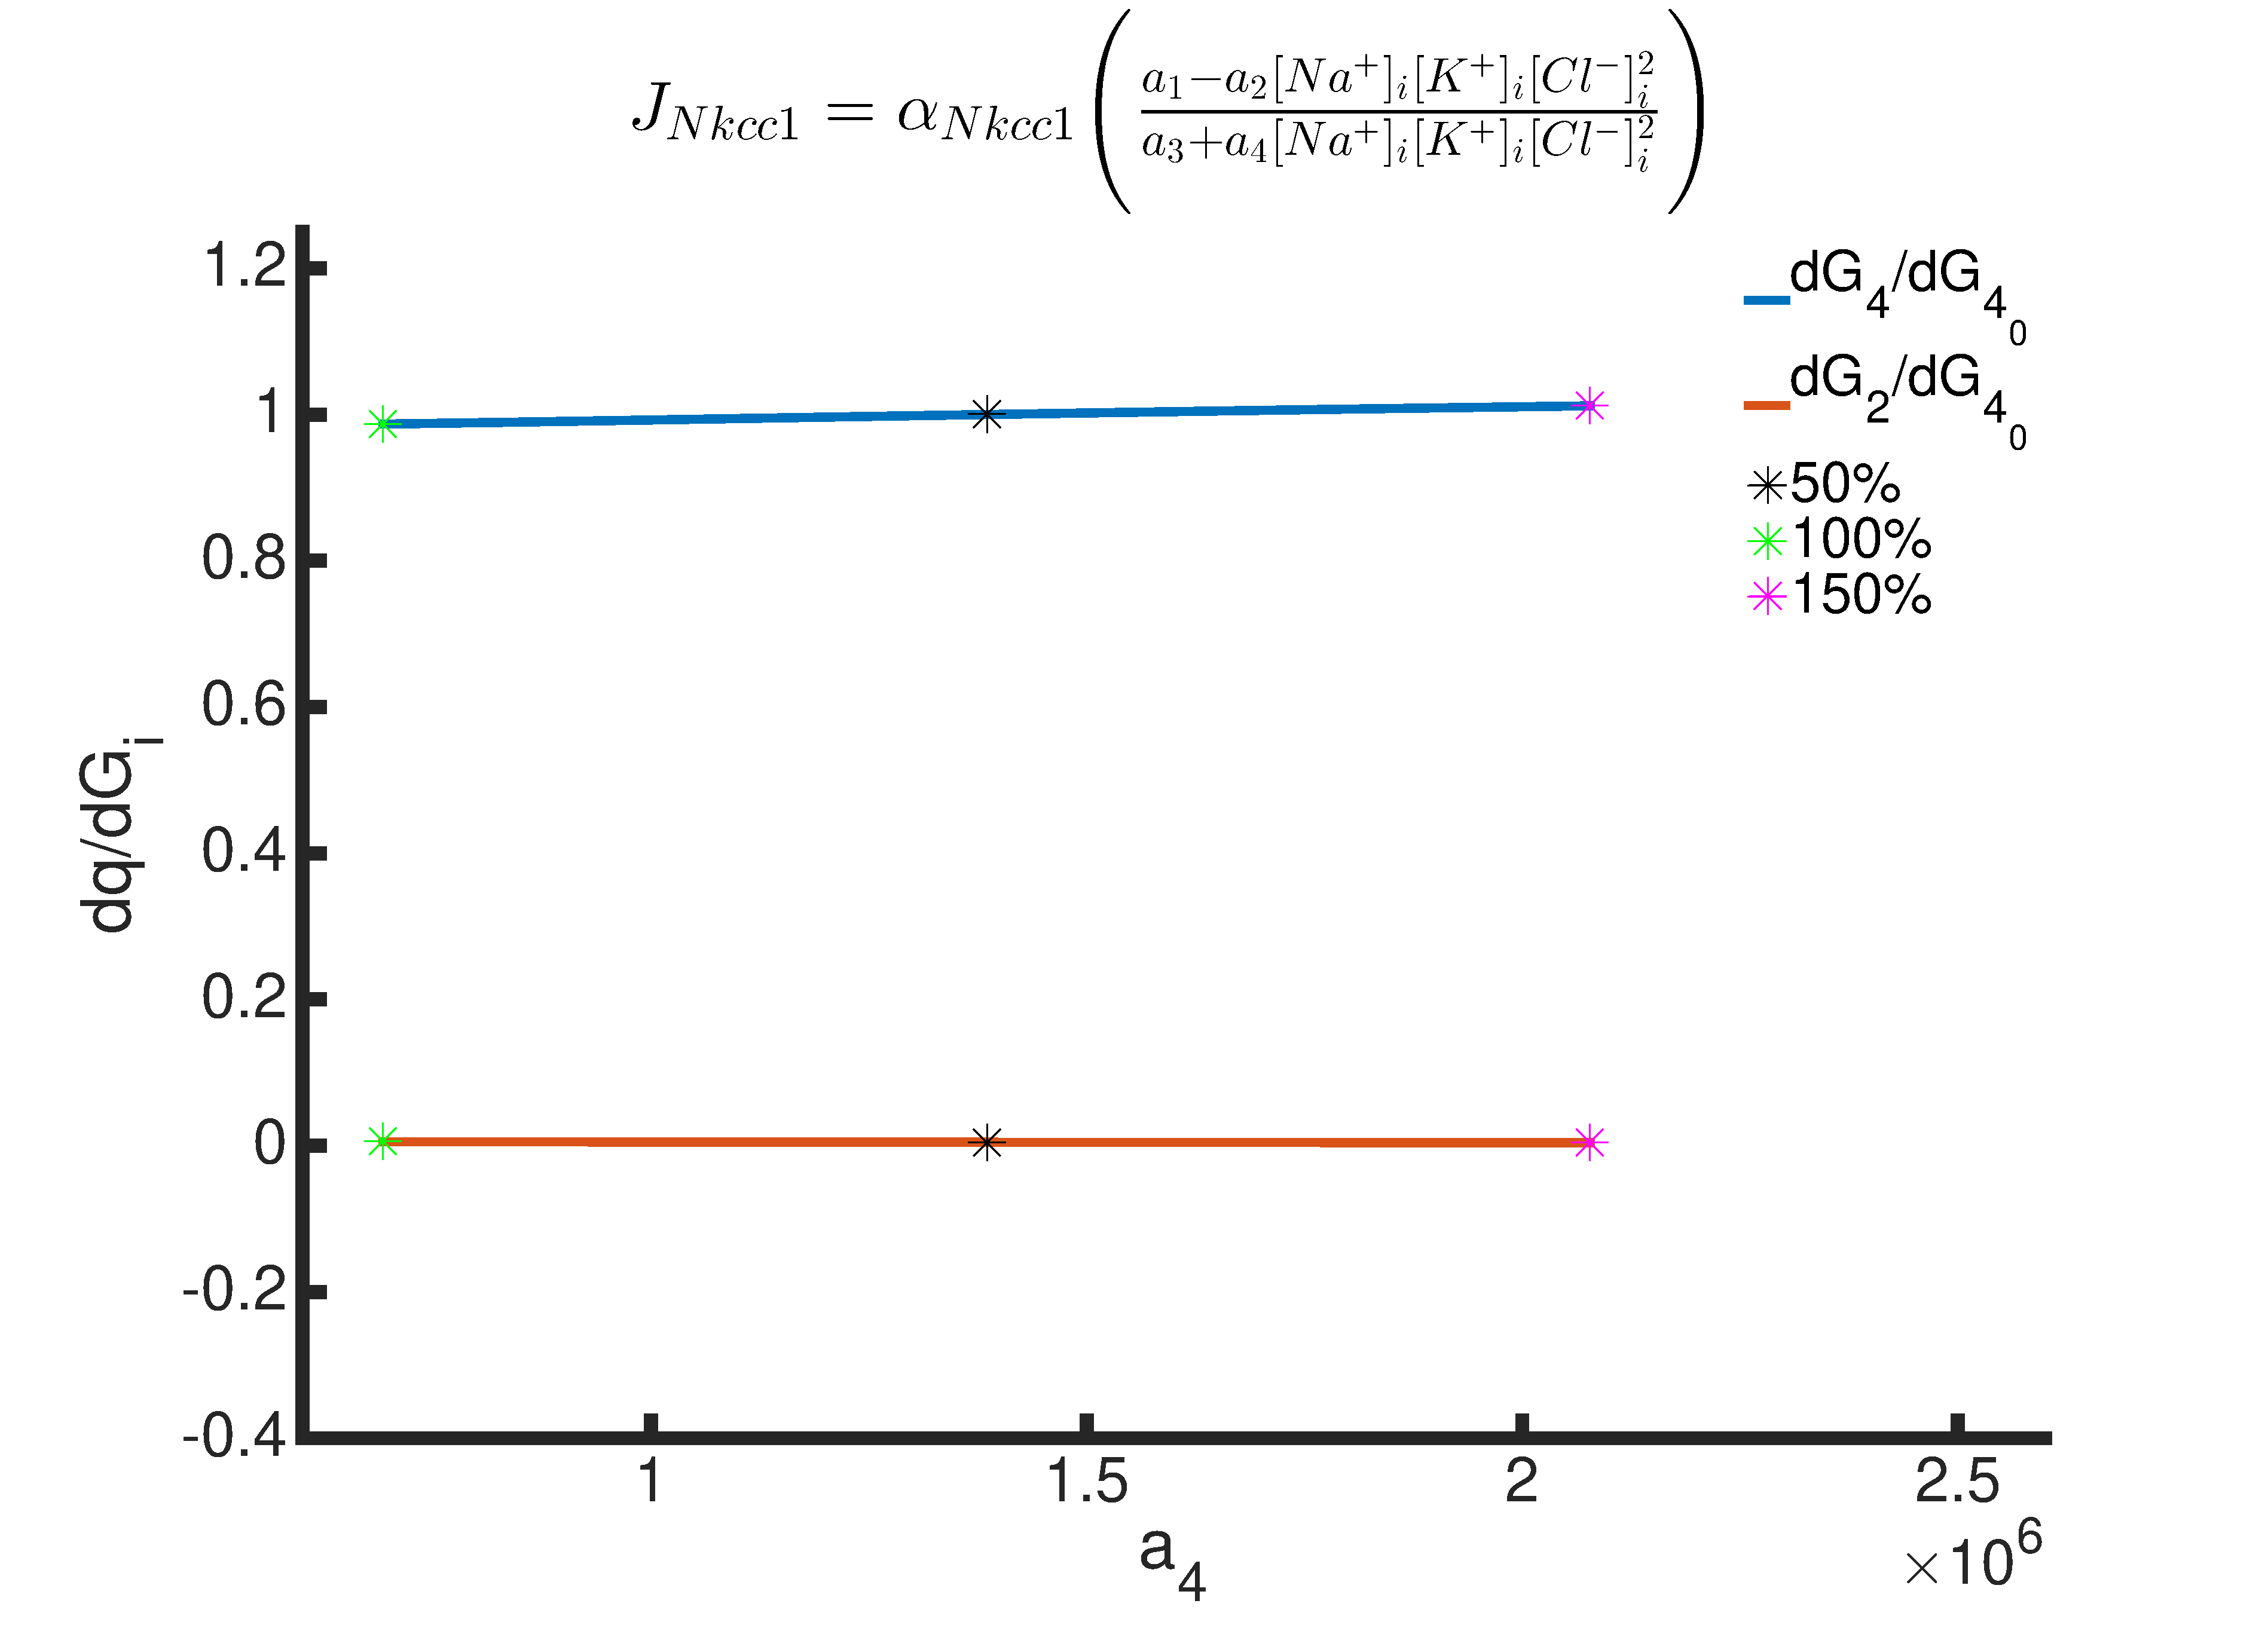
\includegraphics[width=\linewidth]{Figure17.eps}
                \label{fig:QH}
        \end{subfigure}  
        \captionsetup{justification=centering} 
        \caption{}
        \label{fig:results}      
\end{figure}
%%%%%%%%%%%%%%%%%%%%%%%%%%%%%%%%%%%%%%%%%%%%%%%%%%%%%%%%%%%%%%%%%%%%%%%%%%%%%%%%%%%%%%%%%%%%%%%%
%%%%%%%%%%%%%%%%%%%%%%%%%%%%%%%%%%%%%%%%%%%%%%%%%%%%%%%%%%%%%%%%%%%%%%%%%%%%%%%%%%%%%%%%%%%%%%%%
%%%%%%%%%%%%%%%%%%%%%%%%%%%%%%%%%%%%%%%%%%%%%%%%%%%%%%%%%%%%%%%%%%%%%%%%%%%%%%%%%%%%%%%%%%%%%%%%


%%%%%%%%%%%%%%%%%%%%%%%%%%%%%%%%%%%%%%%%%%%%%%%%%%%%%%%%%%%%%%%%%%%%%%%%%%%%%%%%%%%%%%%%%%%%%%%%
%%%%%%%%%%%%%%%%%%%%%%%%%%%%%%%%%%%%%%%%%%%%%%%%%%%%%%%%%%%%%%%%%%%%%%%%%%%%%%%%%%%%%%%%%%%%%%%%
%%%%%%%%%%%%%%%%%%%%%%%%%%%%%%%%%%%%%%%%%%%%%%%%%%%%%%%%%%%%%%%%%%%%%%%%%%%%%%%%%%%%%%%%%%%%%%%%
\begin{figure}
\centering
        \begin{subfigure}{0.49\textwidth}
				\caption{\qquad}                
                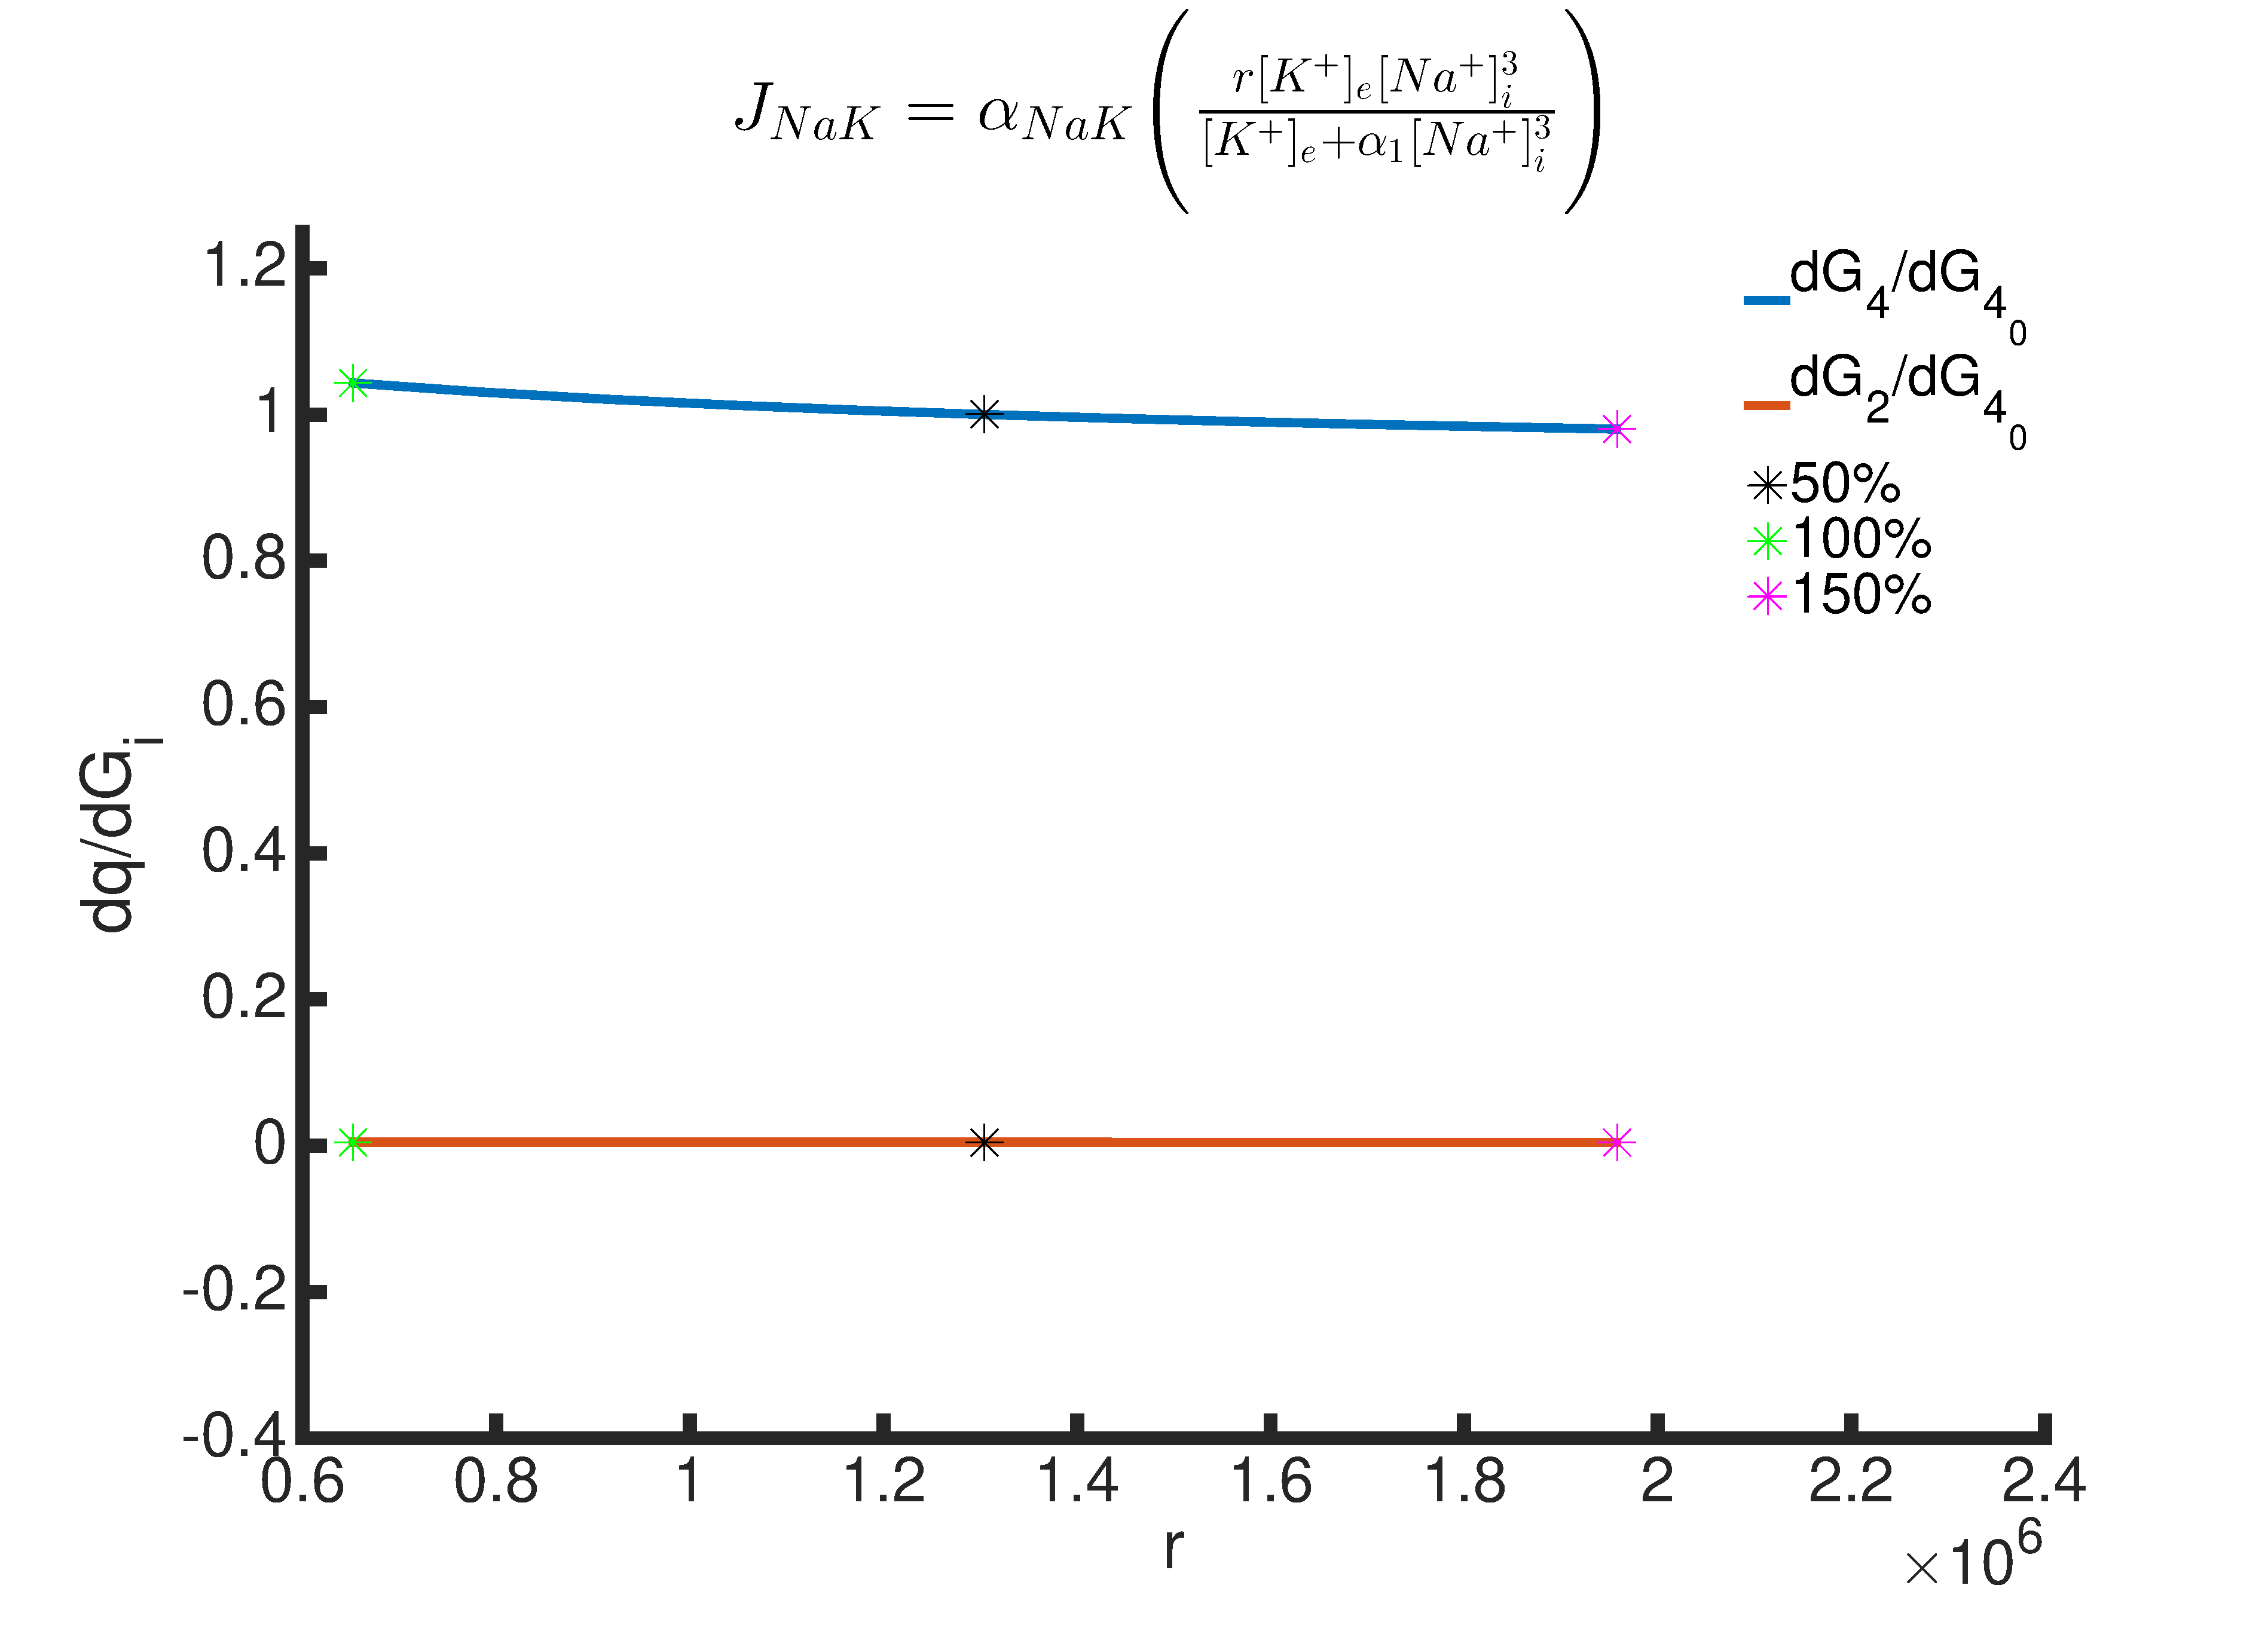
\includegraphics[width=\linewidth]{Figure18.eps}
                \label{fig:det_G2}
        \end{subfigure}
        \begin{subfigure}{0.49\textwidth}
        			\caption{\qquad}
                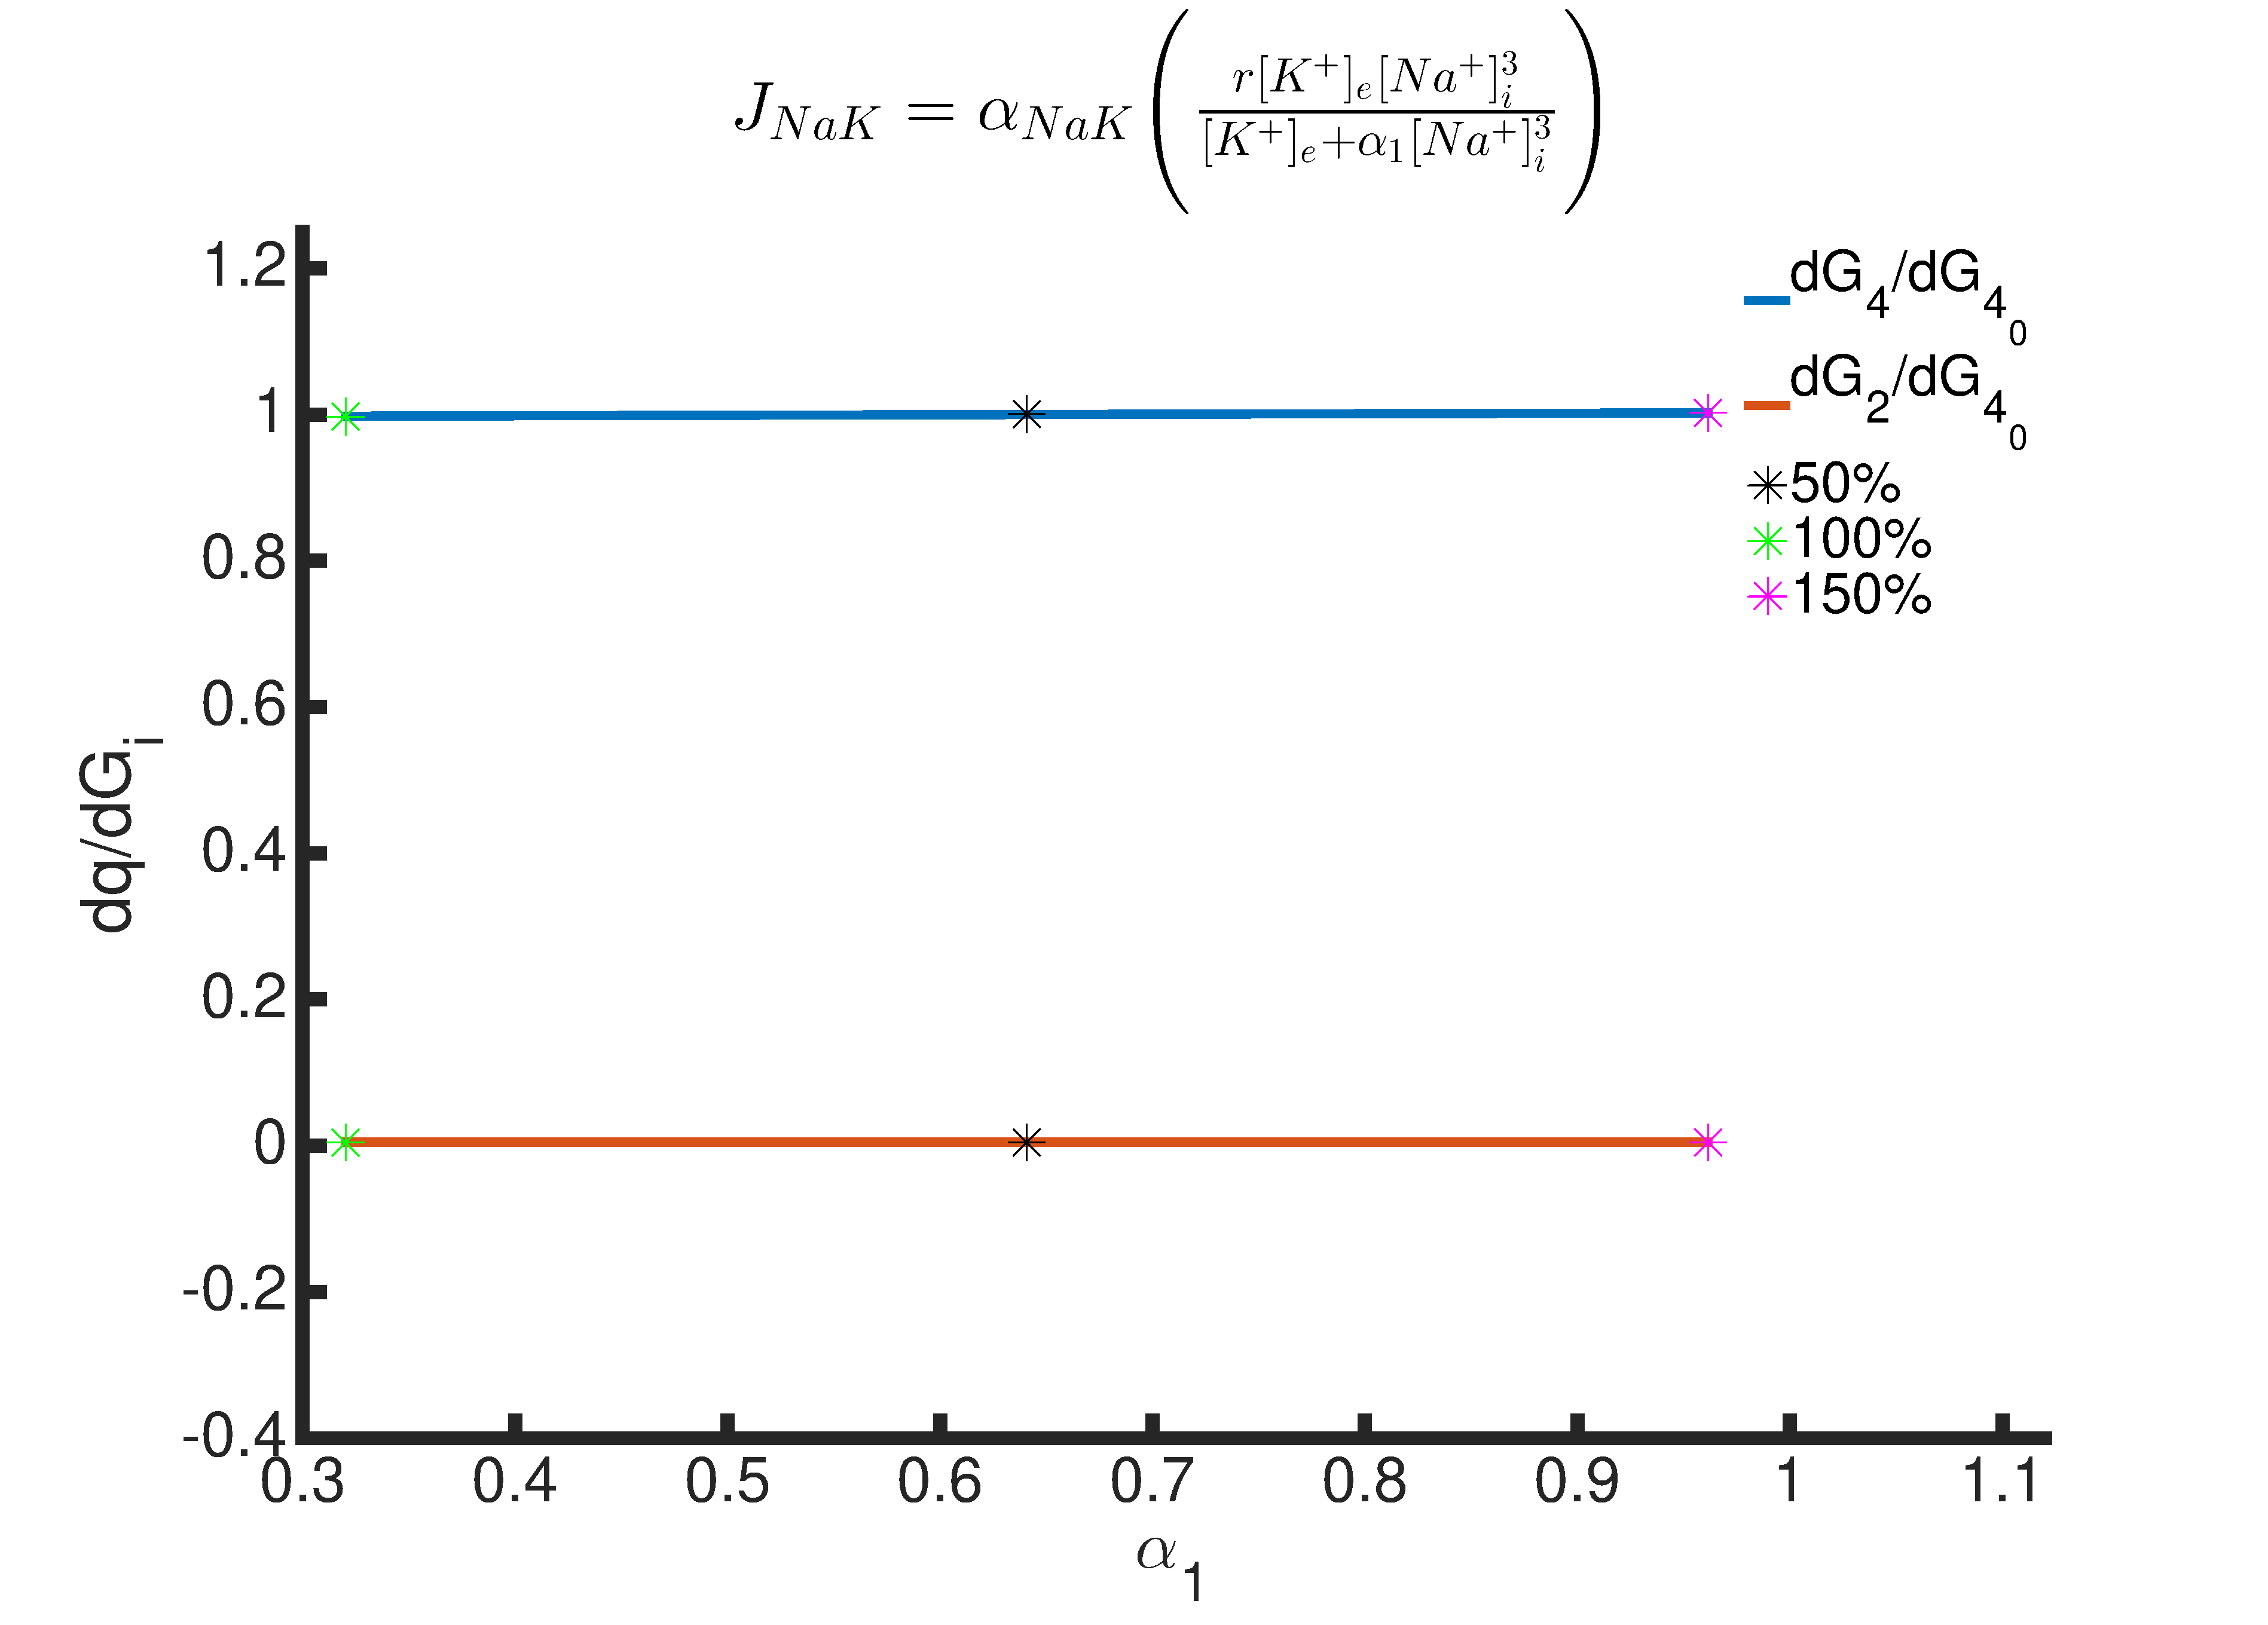
\includegraphics[width=\linewidth]{Figure19.eps}
                \label{fig:det_G4}
        \end{subfigure}     
		           
        
        \begin{subfigure}{0.49\textwidth}
				\caption{\qquad}                
                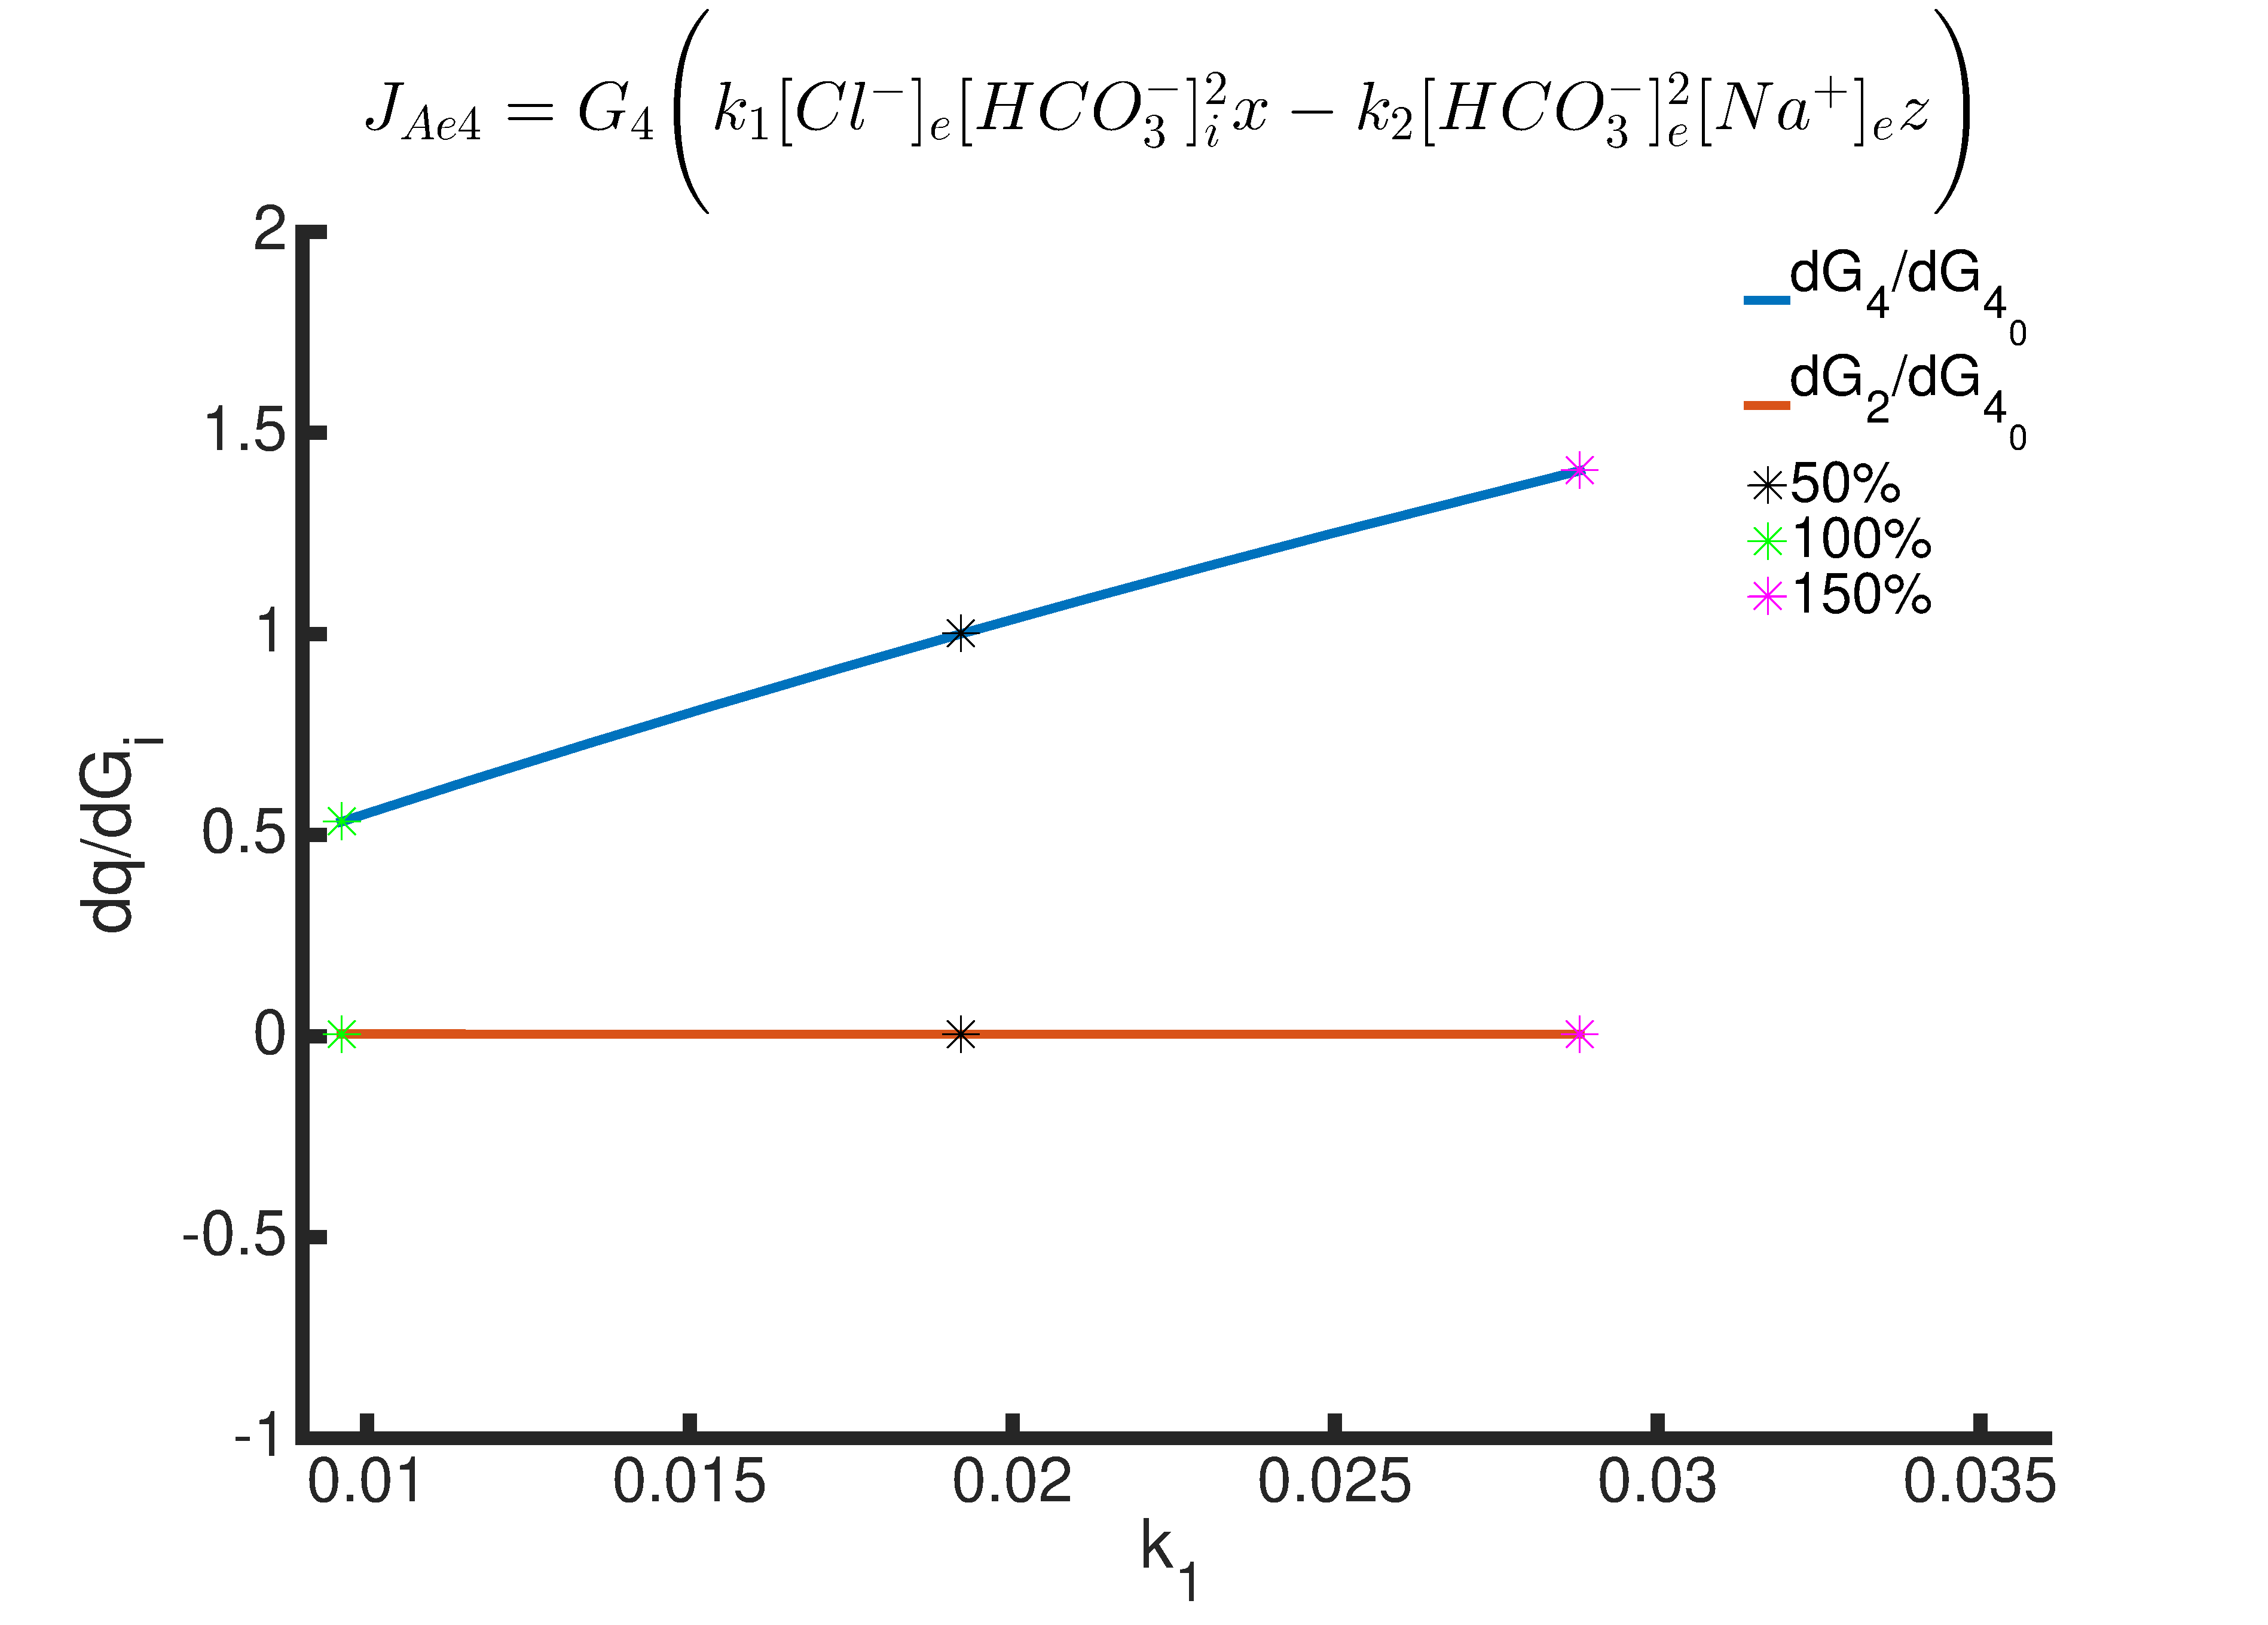
\includegraphics[width=\linewidth]{Figure8.eps}
                \label{fig:xyzG2}
        \end{subfigure}
       \begin{subfigure}{0.49\textwidth}
       			\caption{\qquad}
                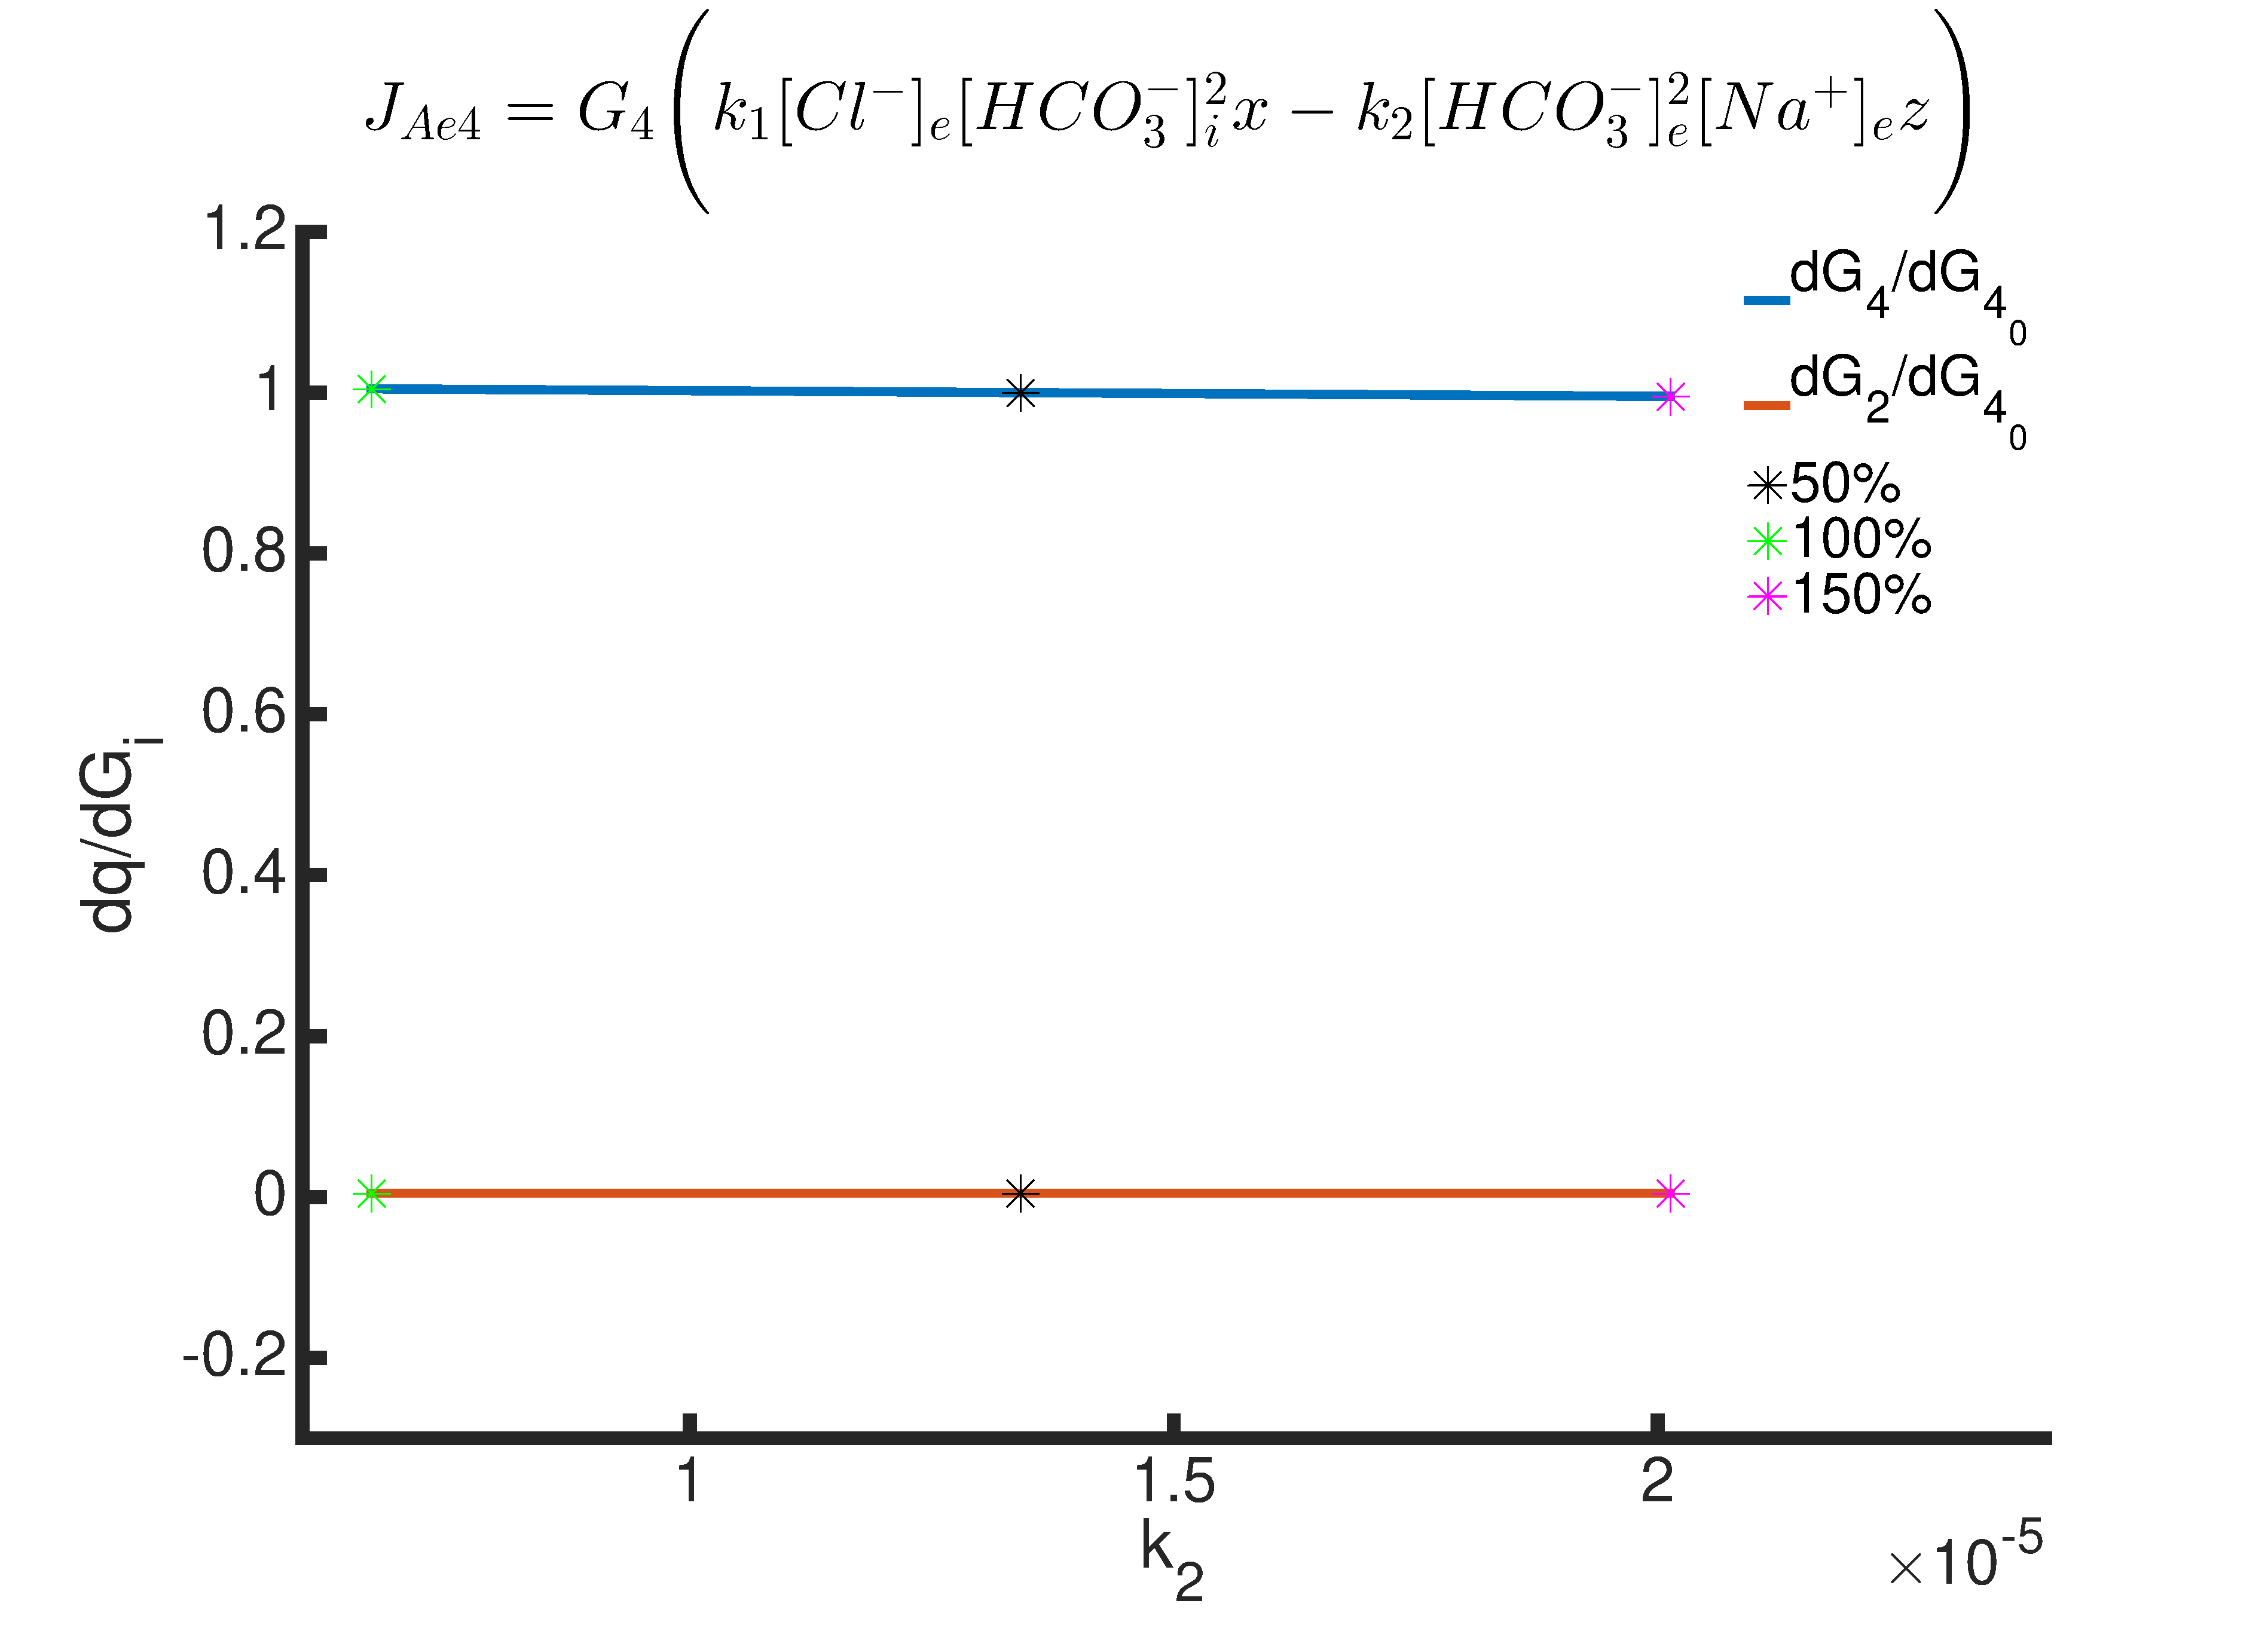
\includegraphics[width=\linewidth]{Figure9.eps}
                \label{fig:xyzG4}
        \end{subfigure}     
        
        \begin{subfigure}{0.49\textwidth}
        			\caption{\qquad}
                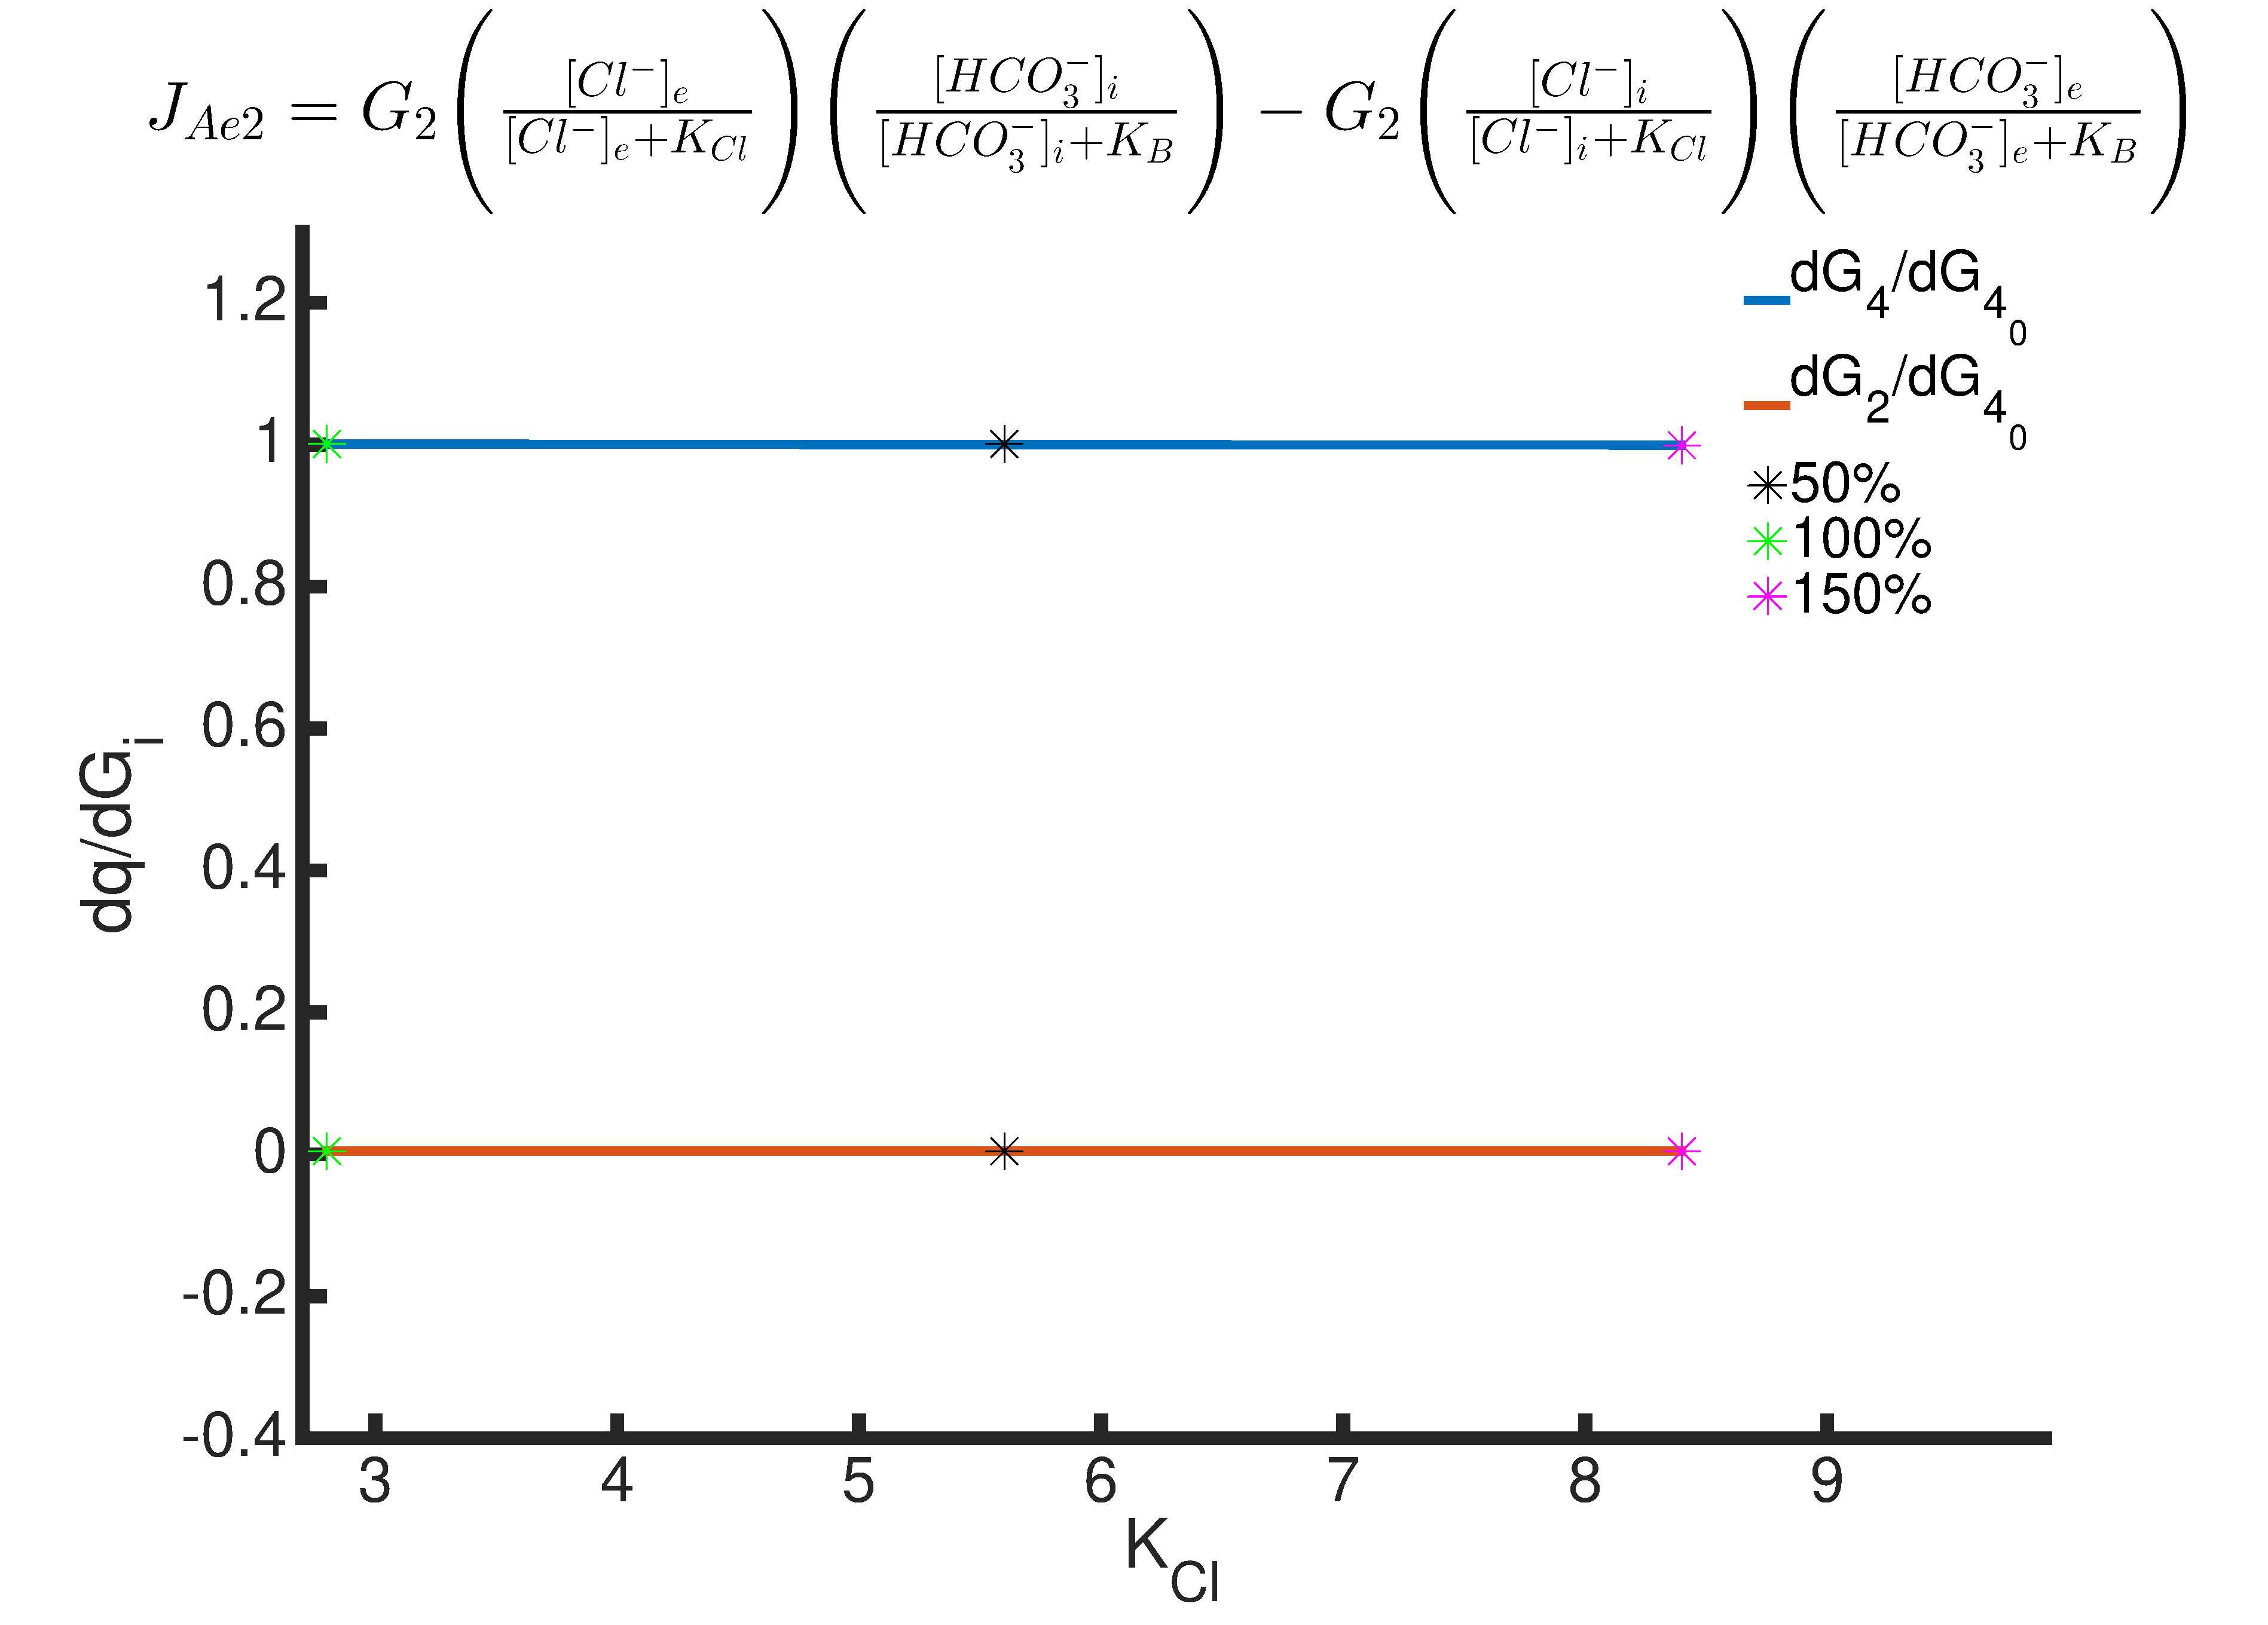
\includegraphics[width=\linewidth]{Figure10.eps}
                \label{fig:Q}
        \end{subfigure}
       \begin{subfigure}{0.49\textwidth}
       			\caption{\qquad}
                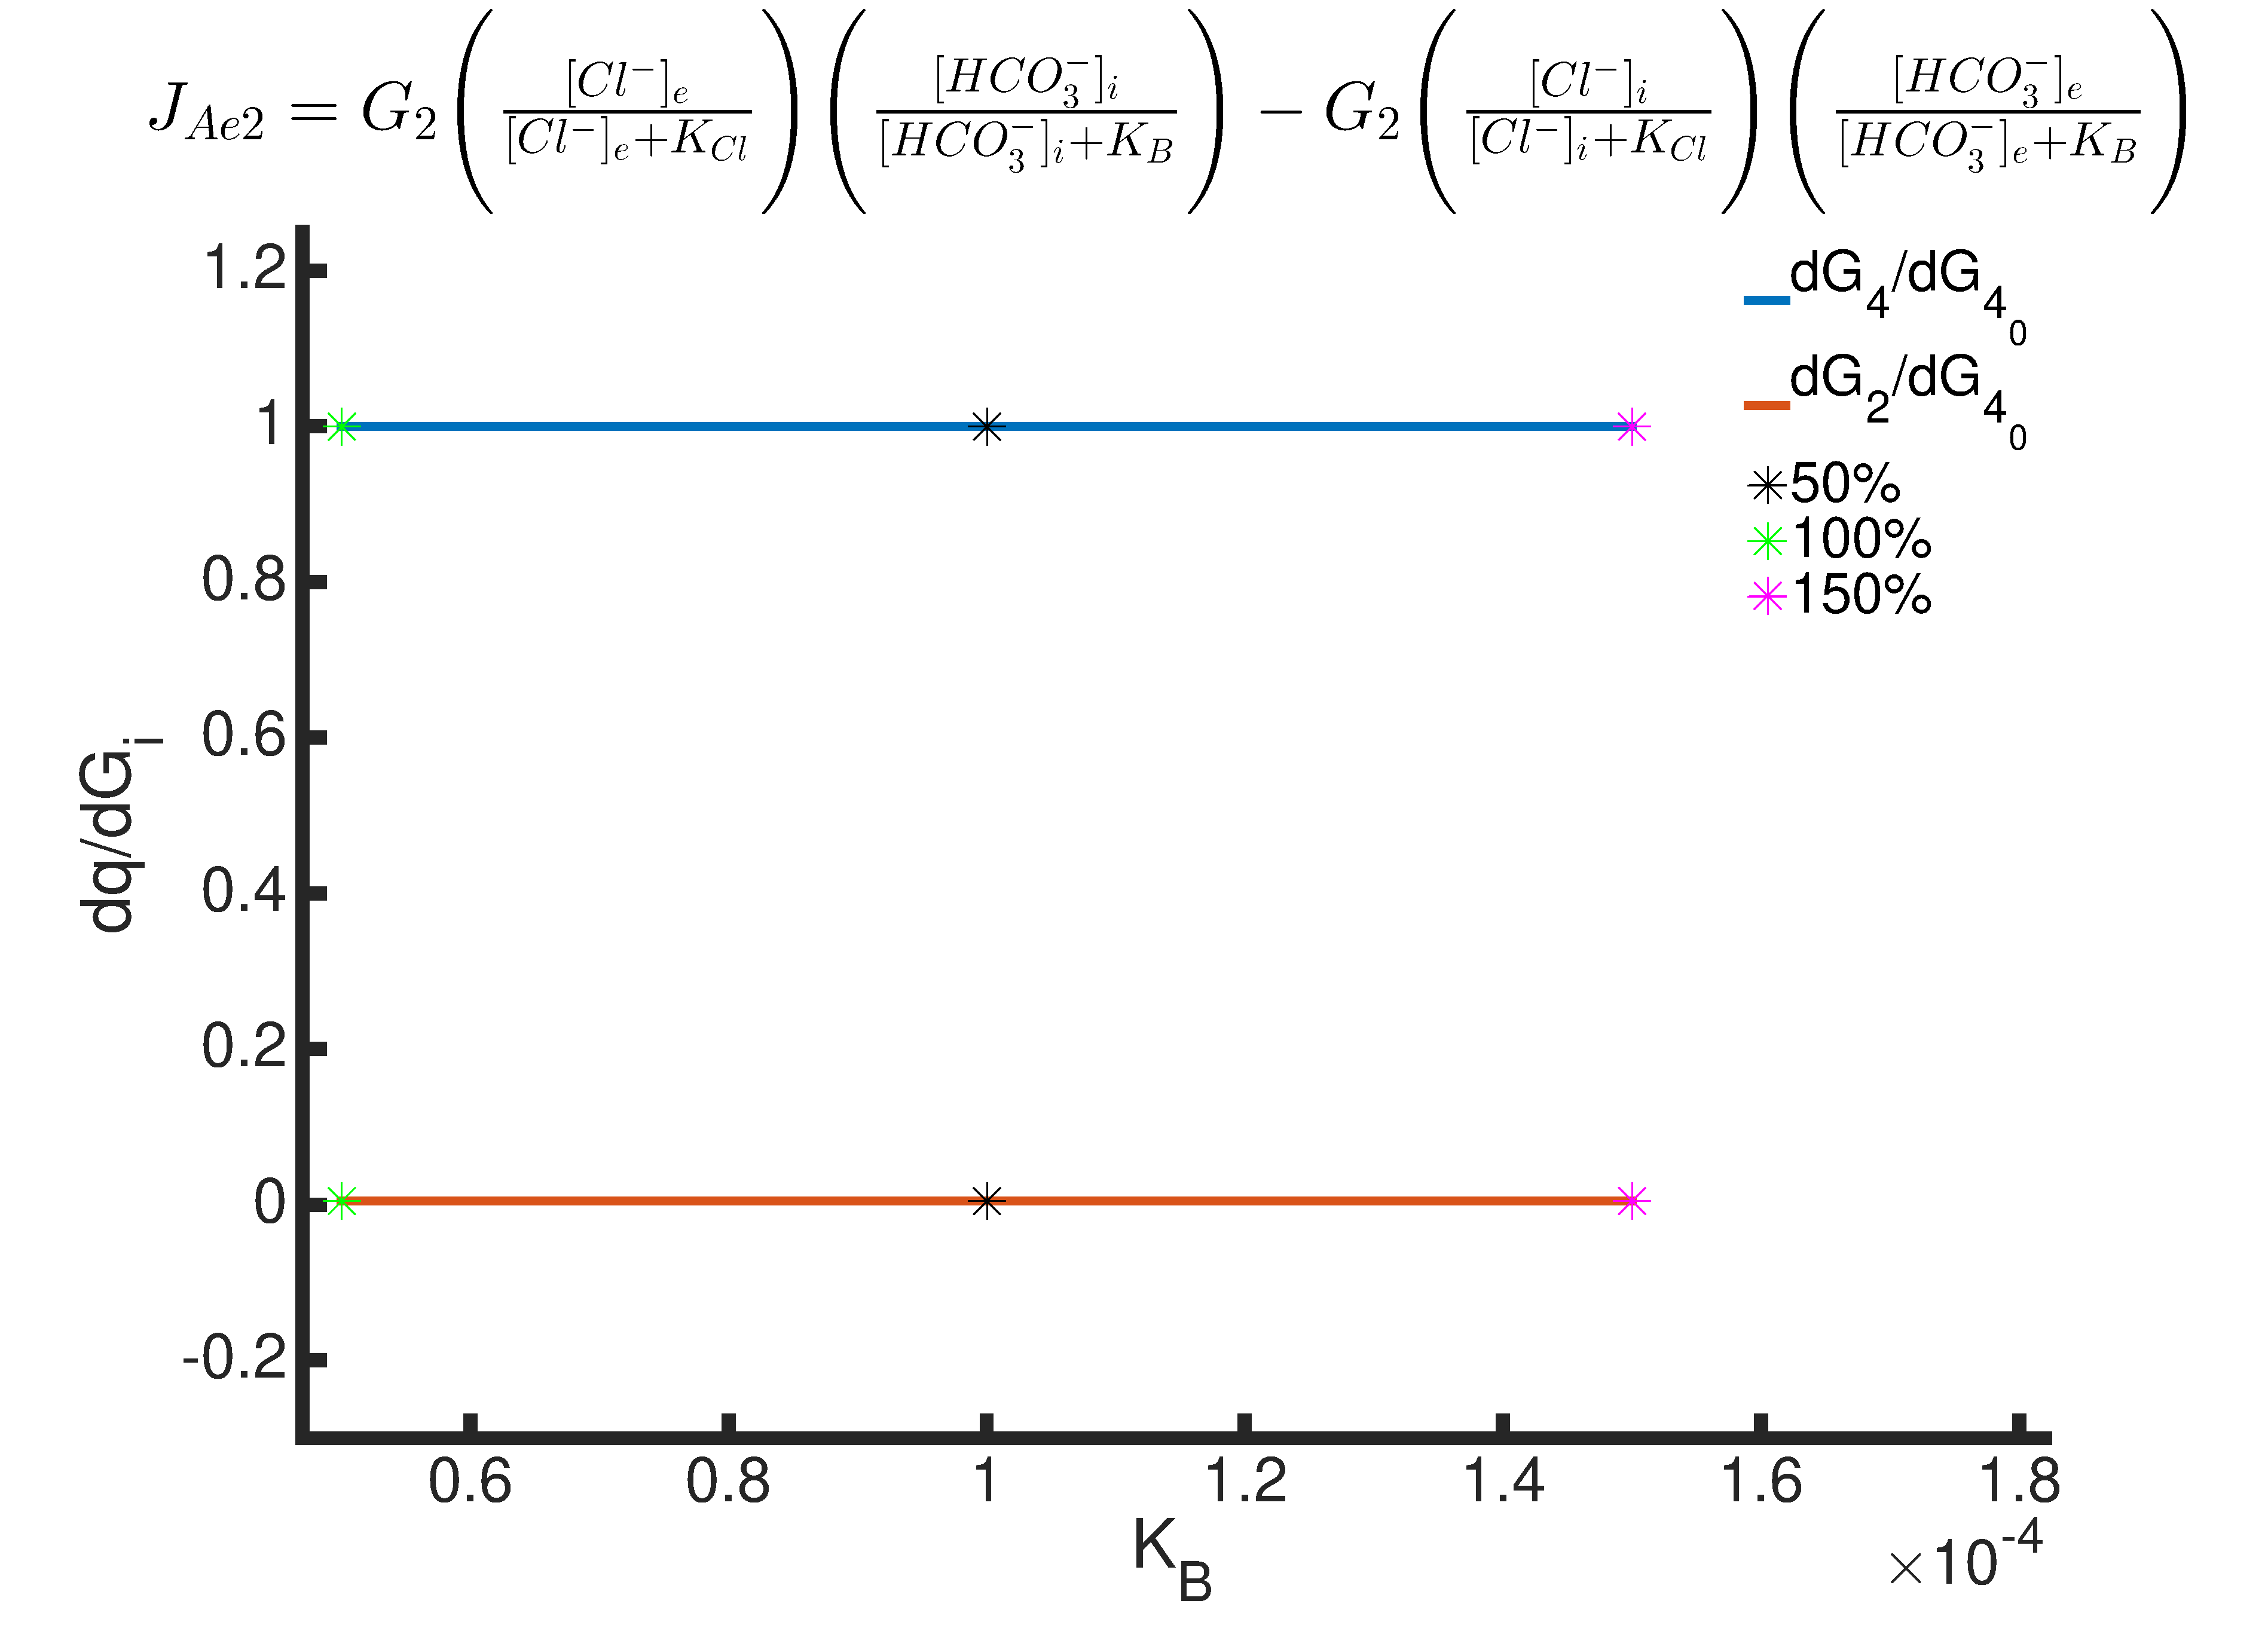
\includegraphics[width=\linewidth]{Figure11.eps}
                \label{fig:QH}
        \end{subfigure}  
        \captionsetup{justification=centering} 
        \caption{}
        \label{fig:results}      
\end{figure}
%%%%%%%%%%%%%%%%%%%%%%%%%%%%%%%%%%%%%%%%%%%%%%%%%%%%%%%%%%%%%%%%%%%%%%%%%%%%%%%%%%%%%%%%%%%%%%%%
%%%%%%%%%%%%%%%%%%%%%%%%%%%%%%%%%%%%%%%%%%%%%%%%%%%%%%%%%%%%%%%%%%%%%%%%%%%%%%%%%%%%%%%%%%%%%%%%
%%%%%%%%%%%%%%%%%%%%%%%%%%%%%%%%%%%%%%%%%%%%%%%%%%%%%%%%%%%%%%%%%%%%%%%%%%%%%%%%%%%%%%%%%%%%%%%%


%%%%%%%%%%%%%%%%%%%%%%%%%%%%%%%%%%%%%%%%%%%%%%%%%%%%%%%%%%%%%%%%%%%%%%%%%%%%%%%%%%%%%%%%%%%%%%%%
%%%%%%%%%%%%%%%%%%%%%%%%%%%%%%%%%%%%%%%%%%%%%%%%%%%%%%%%%%%%%%%%%%%%%%%%%%%%%%%%%%%%%%%%%%%%%%%%
%%%%%%%%%%%%%%%%%%%%%%%%%%%%%%%%%%%%%%%%%%%%%%%%%%%%%%%%%%%%%%%%%%%%%%%%%%%%%%%%%%%%%%%%%%%%%%%%
\begin{figure}
\centering
        \begin{subfigure}{0.49\textwidth}
        			\caption{\qquad}
                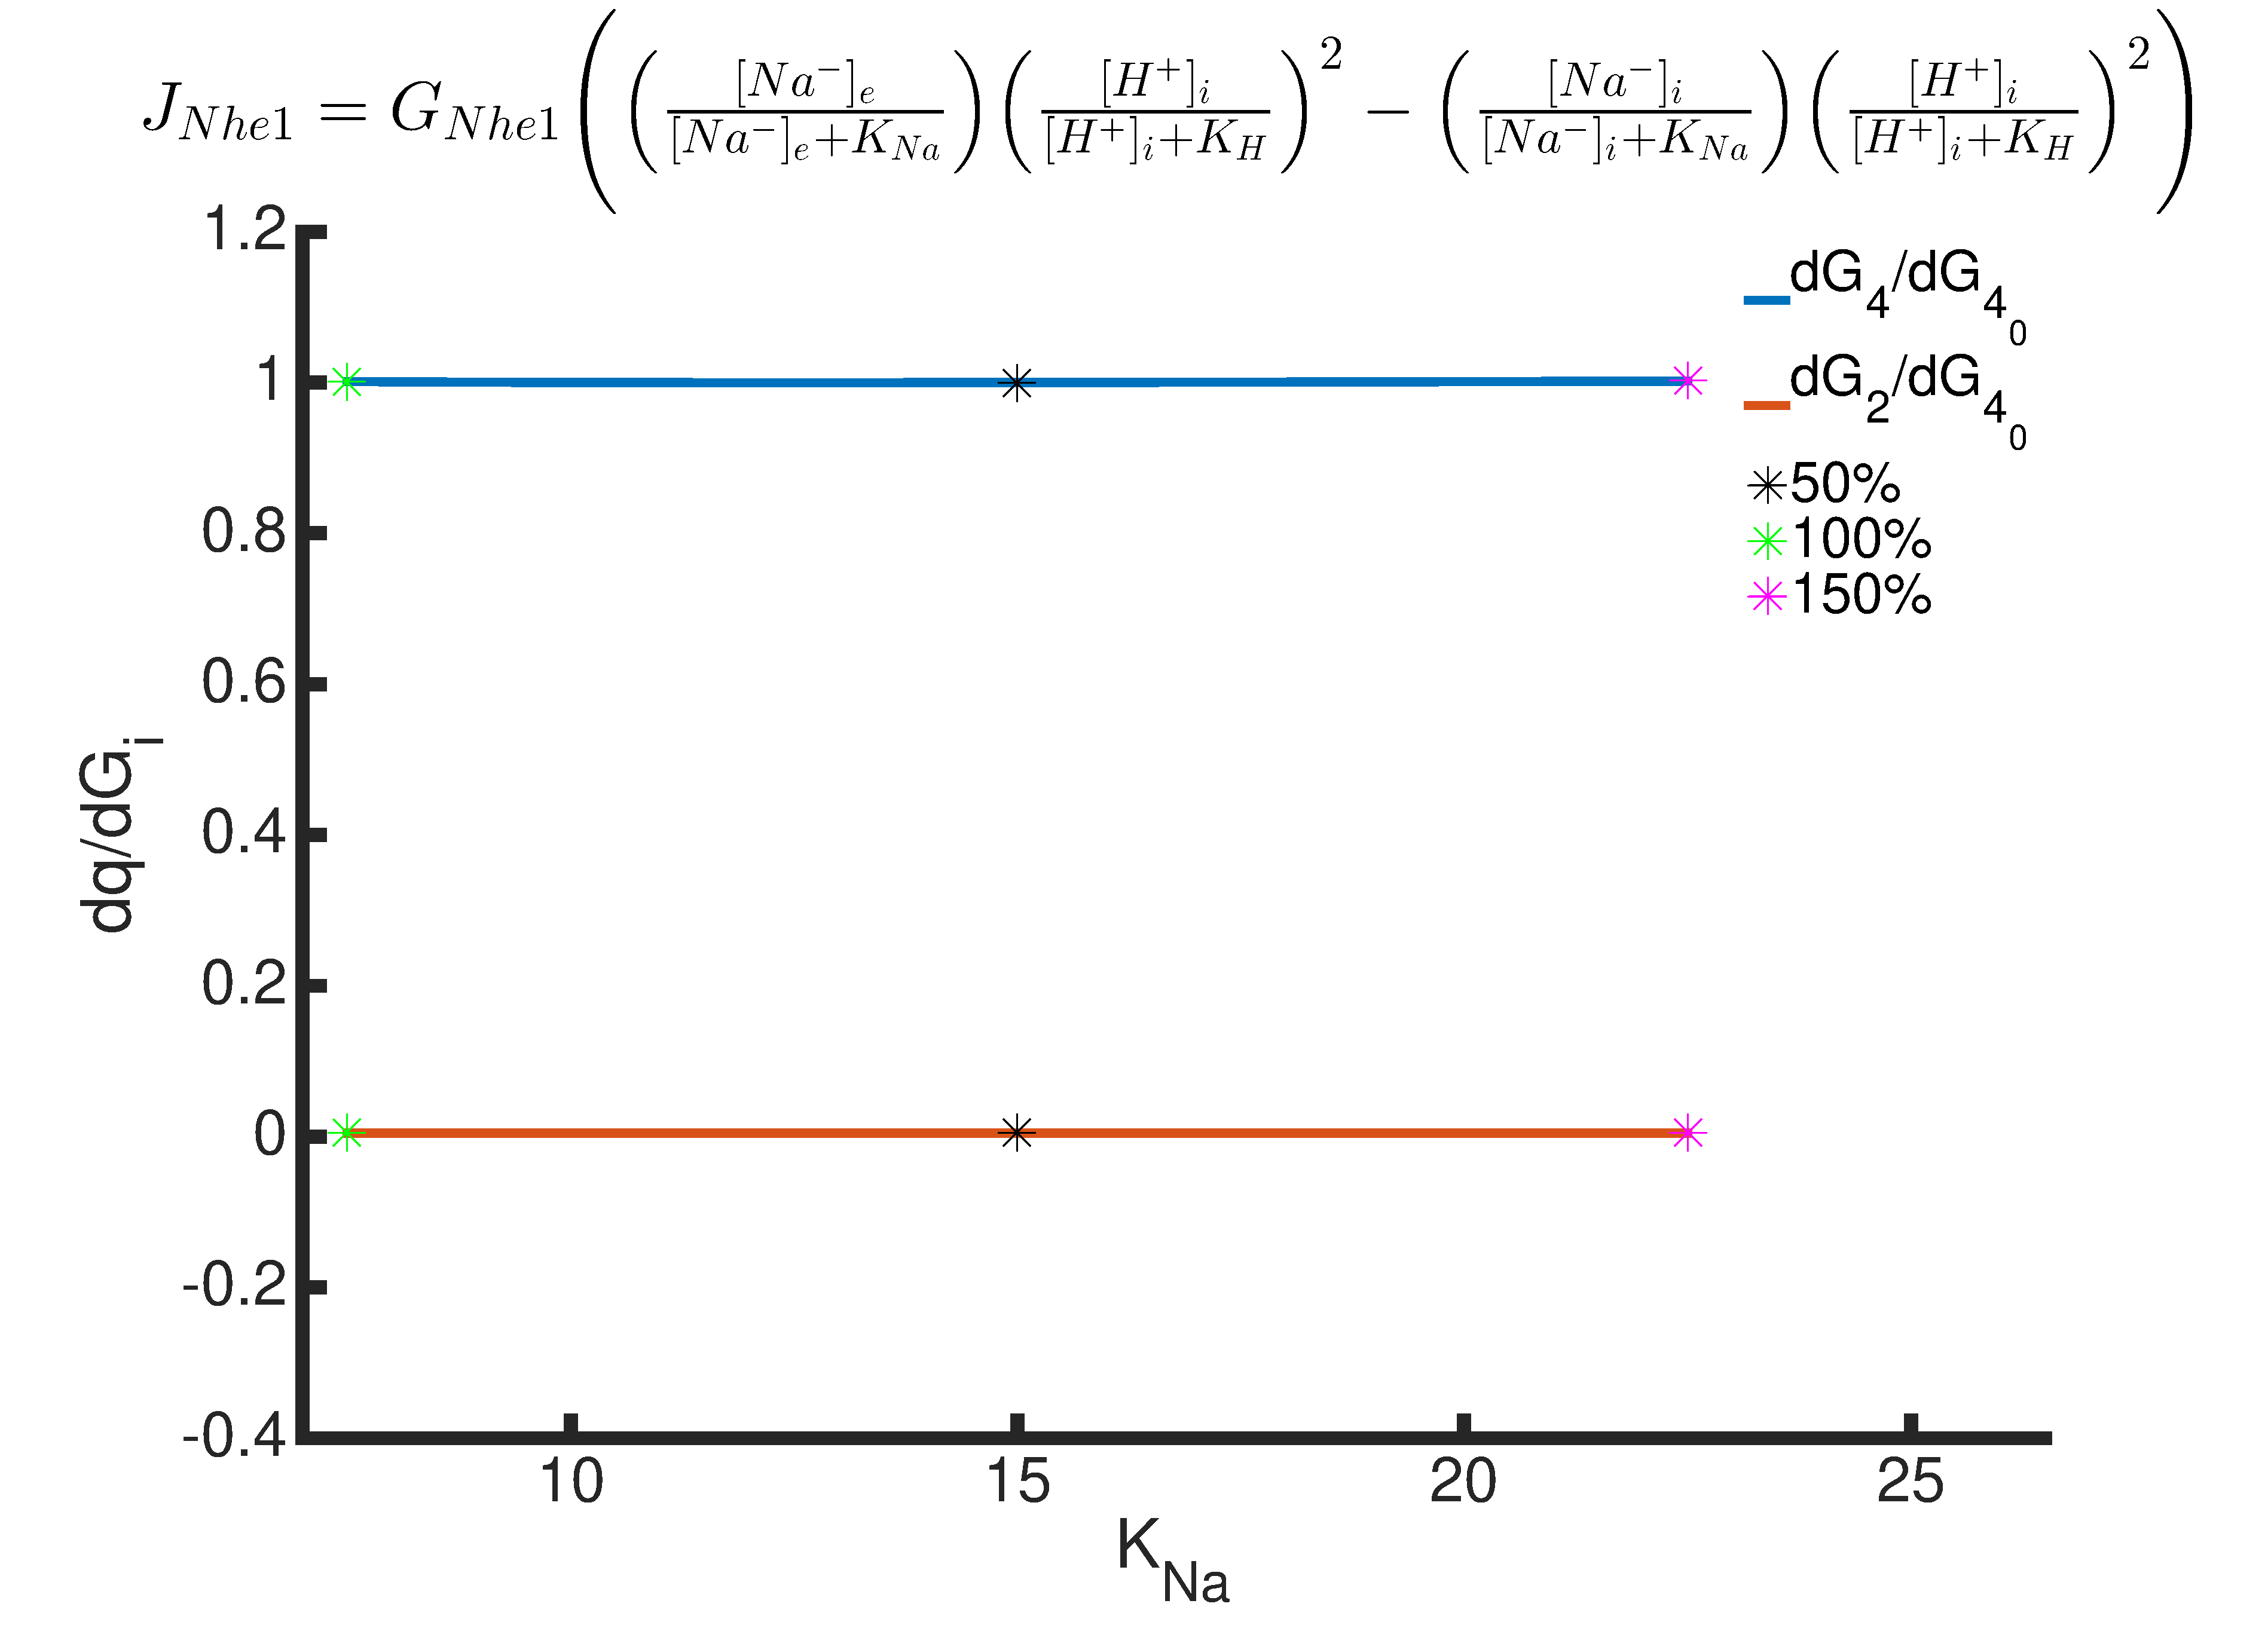
\includegraphics[width=\linewidth]{Figure12.eps}
                \label{fig:det_G2}
        \end{subfigure}
       \begin{subfigure}{0.49\textwidth}
       			\caption{\qquad}
                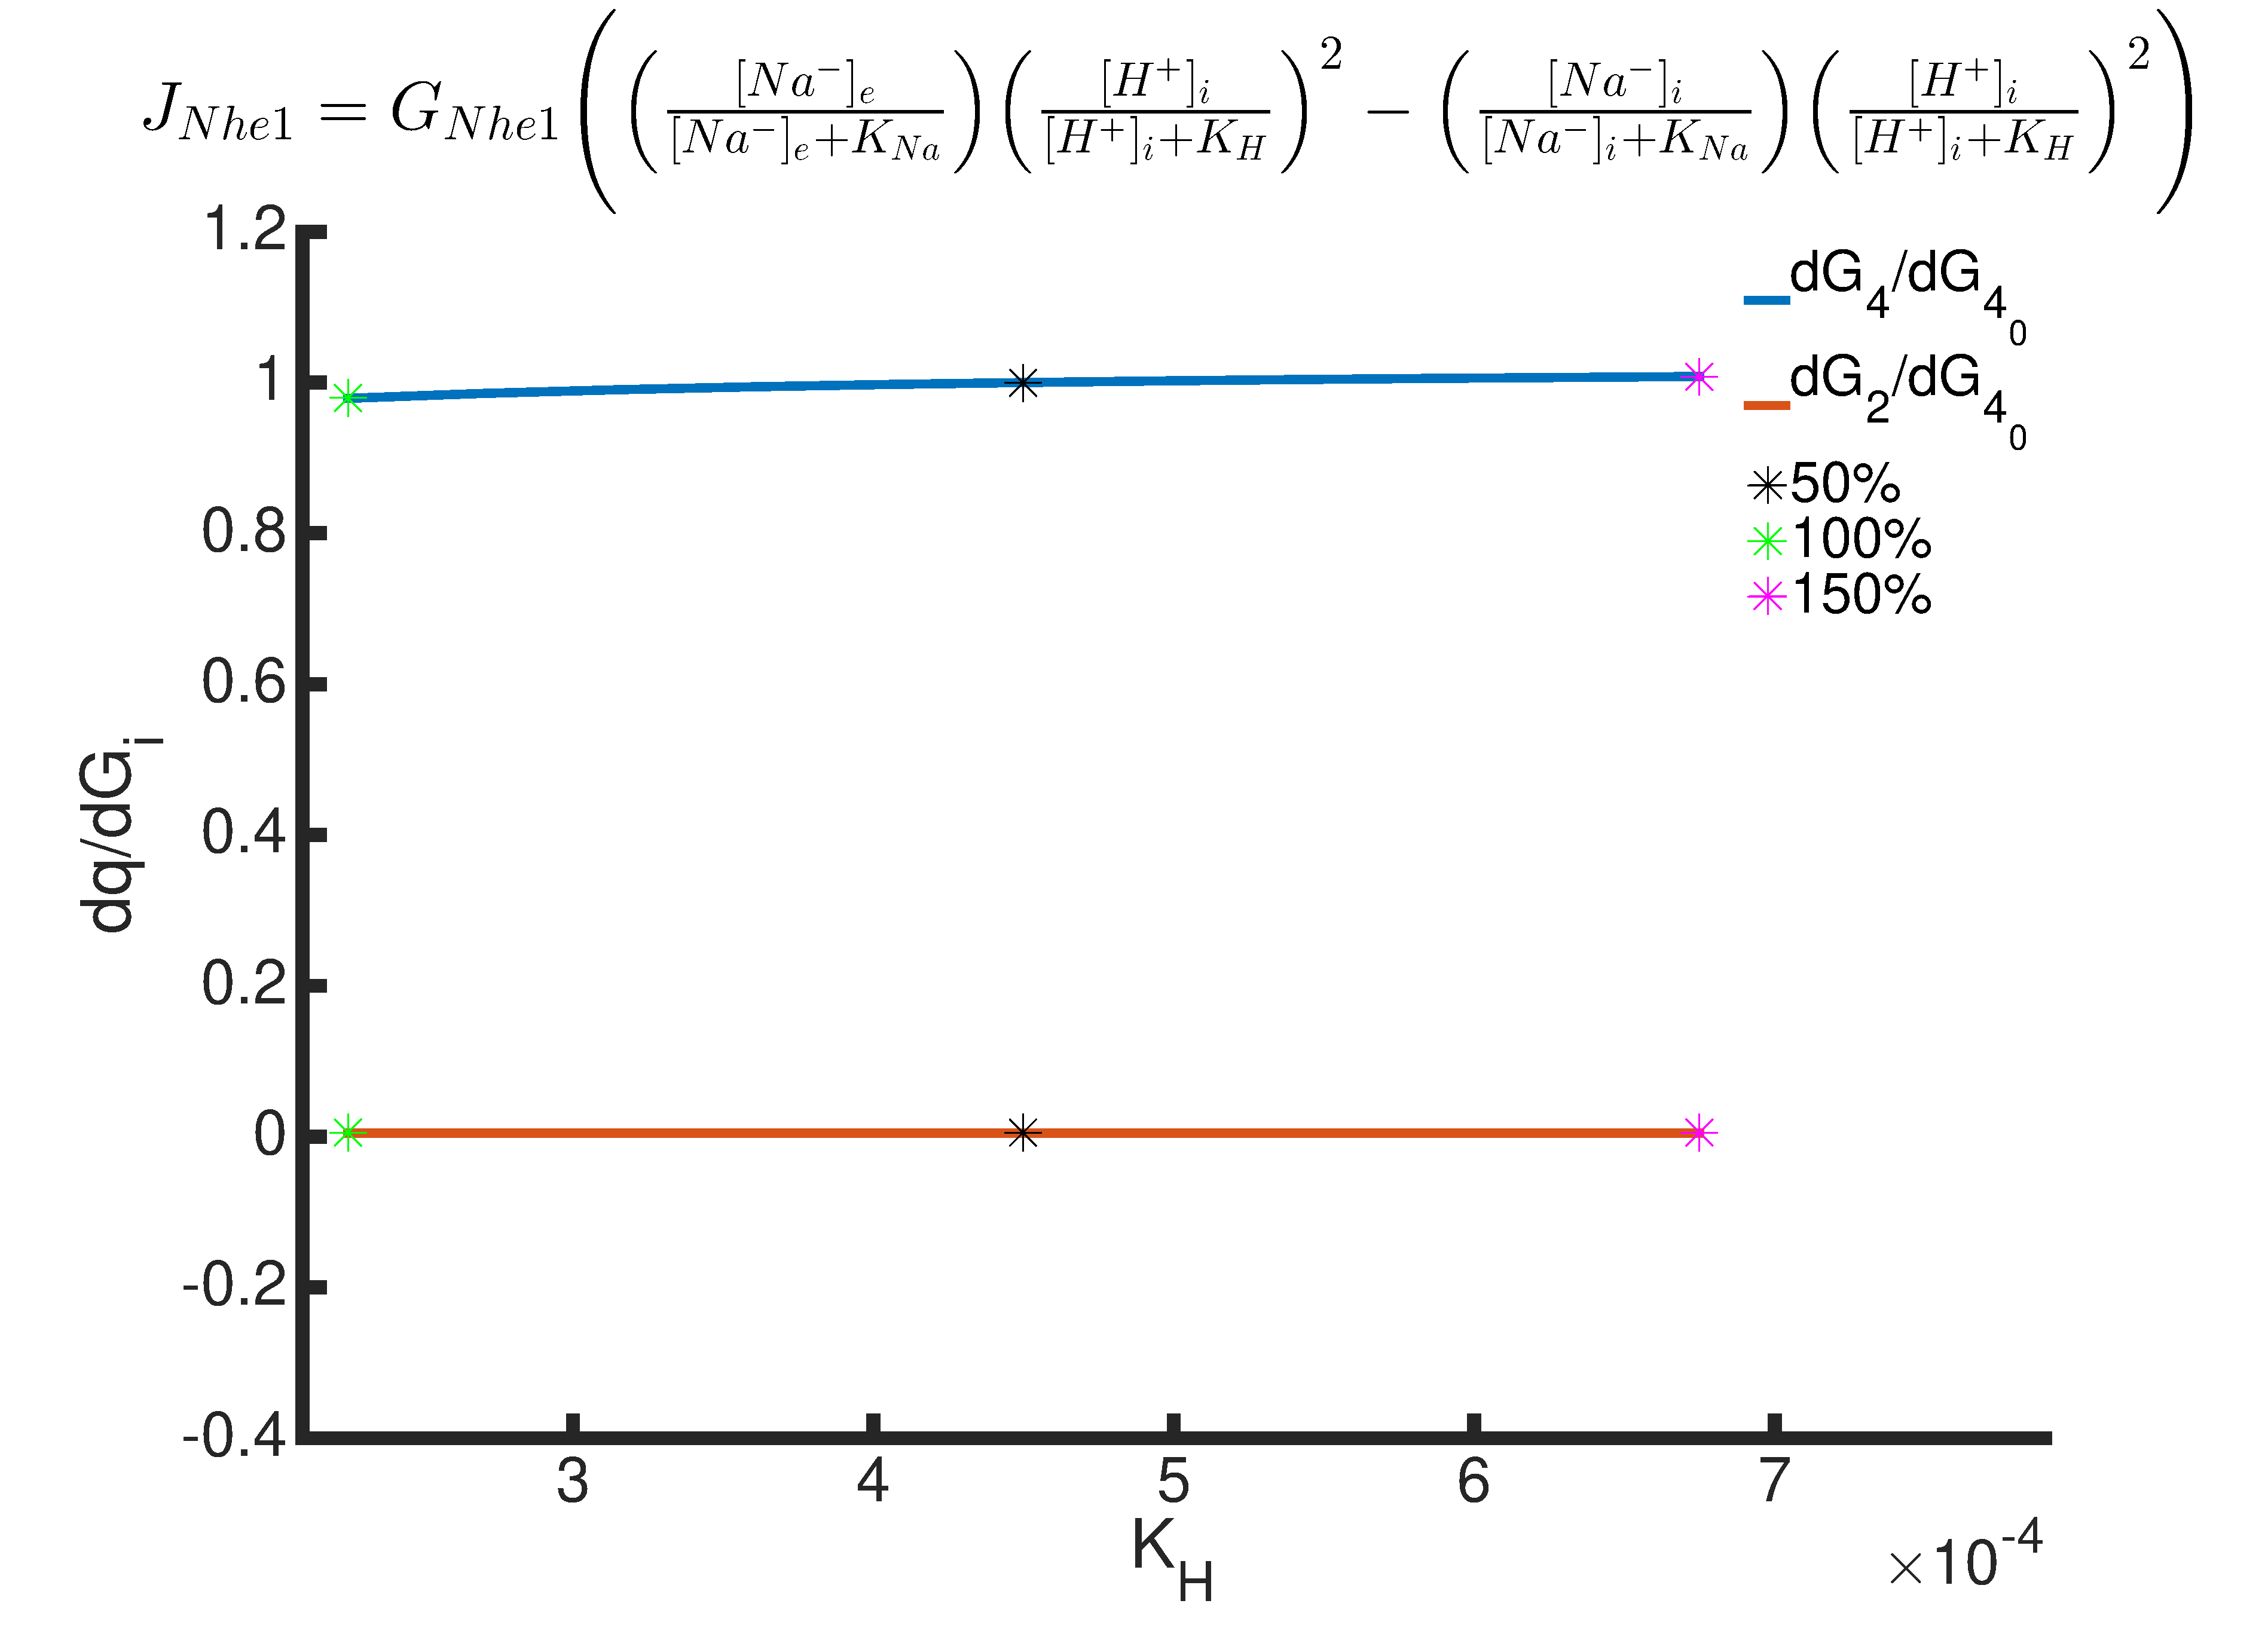
\includegraphics[width=\linewidth]{Figure13.eps}
                \label{fig:det_G4}
        \end{subfigure}
        \captionsetup{justification=centering} 
        \caption{}
        \label{fig:results}      
\end{figure}
%%%%%%%%%%%%%%%%%%%%%%%%%%%%%%%%%%%%%%%%%%%%%%%%%%%%%%%%%%%%%%%%%%%%%%%%%%%%%%%%%%%%%%%%%%%%%%%%
%%%%%%%%%%%%%%%%%%%%%%%%%%%%%%%%%%%%%%%%%%%%%%%%%%%%%%%%%%%%%%%%%%%%%%%%%%%%%%%%%%%%%%%%%%%%%%%%
%%%%%%%%%%%%%%%%%%%%%%%%%%%%%%%%%%%%%%%%%%%%%%%%%%%%%%%%%%%%%%%%%%%%%%%%%%%%%%%%%%%%%%%%%%%%%%%%

\clearpage
\appendix
\title{\Large \bf{Appendix}}
\section*{\Large Nkcc1}

The steady state flux through the Nkcc1 cotransporter is given by,
\begin{align*}
j_{\text{Nkcc1}}= \alpha_{\text{Nkcc1}} \Bigg( \frac{a_1-a_2 \bna \bkplus \bcl^2}{a_3+a_4\bna \bkplus \bcl^2} \Bigg),
\end{align*}
where $\alpha_{\text{Nkcc1}}$ is the cotransporter's density. Following the non-dimensionalisation steps in section ... we arrive at the non-dimensional flux,
\begin{align}
j_{\text{Nkcc1}}= \Bigg( \frac{\lambda_1-\lambda_2 (xyz^2)}{\lambda_3+\lambda_4 (xyz^2)} \Bigg).
\end{align}

\begin{table}[H]
\centering
\captionsetup{justification=centering} 
\caption{Parameters of the model.}
\begin{adjustbox}{max width=1.0\textwidth}
\begin{tabular}{@{}ll@{}}
\toprule
\bf{Parameter}				& \bf{Value}							\\ \midrule
$\alpha_{\text{Nkcc1}}$		& 7.21	 (fmol / $\mu \text{m}^3$)	\\
$a_1$ 						& 157.5	 (s$^{-1}$)					\\	
$a_2$						& 2.0096	$\times×10^7$ (mM$^4 \text{s}^{-1}$)	\\
$a_3$ 						& 1.0306	 (s$^{-1}$)	 				\\
$a_4$ 						& 1.3852	$\times×10^6$ (mM$^4 \text{s}^{-1}$)	\\
\bottomrule
\end{tabular}
\end{adjustbox}
\label{table:Nkcc1}
\end{table}

\section*{\Large $\na$ $\kplus$-ATPase}

The steady state flux through the NaK-ATPase pump is given by,
\begin{align*}
j_{\text{NaK}}=\alpha_{\text{NaK}} \Bigg(\frac{r [\kplus]_e^2 \bna^3}{[\kplus]_e^2 + \alpha \bna^3} \Bigg),
\end{align*}
where $\alpha_{\text{Nkcc1}}$ is the cotransporter's density. Following the non-dimensionalisation steps in section ... we arrive at the non-dimensional flux,
\begin{align}
j_{\text{NaK}}=\frac{\lambda_5 x^3}{\lambda_6 +\lambda_7 x^3}.
\end{align}

\begin{table}[H]
\centering
\captionsetup{justification=centering} 
\caption{Parameters of the model.}
\begin{adjustbox}{max width=1.0\textwidth}
\begin{tabular}{@{}ll@{}}
\toprule
\bf{Parameter}				& \bf{Value}										\\ \midrule
$\alpha_{\text{NaK}}$		& 0.93	(fmol / $\mu \text{m}^3$)				\\
$r$ 							& 1.305 $\times 10^6	$ (mM$^3 \text{s}^{-1}$)		\\	
$\alpha$						& 0.641	(mM$^{-1}$)								\\
\bottomrule
\end{tabular}
\end{adjustbox}
\label{table:NaK}
\end{table}

\section*{\Large $\ca$-activated $\kplus$ channels (CaKC)}
The open probability of the CaKC channels is given by,
\begin{align*}
P_{\text{CaKC}}= \Bigg( \frac{\bc}{\bc+K_{\text{CaKC}} } \Bigg)^{\eta_2},
\end{align*}
where $\eta_2=2.54$ is the Hill coefficient and $K_{\text{CaKC}}=0.182 \ \mu \text{M}$. Note that $P_{\text{CaKC}}$ is already non-dimensional. The flux is defined as,
\begin{align*}
j_{\text{CaKC}}=\frac{G_{CaKC}P_{\text{CaKC}}}{F}\Big( V_{b}-V_{\text{CaKC}} \Big),
\end{align*}
where $V_{\text{CaKC}}$ is the Nernst potential defined by,
\begin{align*}
V_{\text{CaKC}} =\frac{RT}{Fz^K}\ln \Bigg(\frac{[\kplus]_e}{\bkplus} \Bigg).
\end{align*}
Here $z^K$ is the ion's valence, $T$ is the temperature in Kelvin, $R$ the universal gas constant in SI units, and $F$ Faraday's constant in SI units. Following the non-dimensionalisation procedure above we obtain,
\begin{align}
j_{\text{CaKC}}=\lambda_8-\lambda_9 \ln(y).
\end{align}

\section*{\Large $\ca$-activated $\cl$ channels (CaCC)}
The open probability of the CaCC channels is given by,
\begin{align*}
P_{\text{CaCC}}= \Bigg( \frac{\bc}{\bc+K_{\text{CaCC}} } \Bigg)^{\eta_1},
\end{align*}
where $\eta_1=1.46$ is the Hill coefficient and $K_{\text{CaKC}}=0.26 \ \mu \text{M}$. Note that $P_{\text{CaCC}}$ is already non-dimensional. The flux is defined as,
\begin{align*}
j_{\text{CaCC}}=\frac{G_{CaCC}P_{\text{CaCC}}}{F}\Big( V_{a}+V_{\text{CaCC}} \Big),
\end{align*}
where $V_{\text{CaCC}}$ is the Nernst potential defined by,
\begin{align*}
V_{\text{CaCC}} =\frac{RT}{Fz^{Cl}}\ln \Bigg(\frac{\blcl}{\bcl} \Bigg).
\end{align*}
Here $z^{Cl}$ is the ion's valence, $T$ is the temperature in Kelvin, $R$ the universal gas constant in SI units, and $F$ Faraday's constant in SI units. Following the non-dimensionalisation procedure above we obtain,
\begin{align}
j_{\text{CaCC}}=\lambda_{10}-\lambda_{11} \ln(z).
\end{align}

\section*{\Large $\hco$/$\cl$ exchanger (Ae2)}
The flux of the transporter is given by,
\begin{align*}
j_{\text{Ae2}}=G_2 \Bigg[ \Bigg( \frac{[\cl]_e}{[\cl]_e + K_{\text{Cl}}} \Bigg)  & \Bigg( \frac{\bhco}{\bhco + K_{\text{B}}}\Bigg) \\
& -\Bigg( \frac{\bcl}{\bcl + K_{\text{Cl}}}\Bigg) \Bigg( \frac{[\hco]_e  }{[\hco]_e + K_{\text{B}}}  \Bigg) \Bigg].
\end{align*}
Following the non-dimensionalisation presented above,
\begin{align}
j_{\text{Ae2}}=\lambda_{12}-\frac{\lambda_{13} z}{z+\lambda_{14}}.
\end{align}
\begin{table}[H]
\centering
\captionsetup{justification=centering} 
\caption{Parameters of the model.}
\begin{adjustbox}{max width=1.0\textwidth}
\begin{tabular}{@{}ll@{}}
\toprule
\bf{Parameter}				& \bf{Value}										\\ \midrule
$G_2$						& 1.92	(amol / $\mu \text{m}^3$ s)				\\
$K_{\text{Cl}}$ 				& 5.6 	(mM)										\\	
$K_{\text{B}}$				& 10$^4$	(mM)										\\
\bottomrule
\end{tabular}
\end{adjustbox}
\label{table:Ae2}
\end{table}

\section*{\Large ($\na$)-$2\hco$/$\cl$ exchanger (Ae4)}
The flux of the transporter is given by,
\begin{align*}
j_{\text{Ae4}}=G_4  \Bigg( k_1 [\cl]_e &\bhco^2 \bna  - k_2 \bcl [\hco]_e^2 [\na]_e\Bigg)\\
\end{align*}
Following the non-dimensionalisation presented above,
\begin{align}
j_{\text{Ae4}}=\lambda_{15}x-\lambda_{16}z.
\end{align}
\begin{table}[H]
\centering
\captionsetup{justification=centering} 
\caption{Parameters of the model.}
\begin{adjustbox}{max width=1.0\textwidth}
\begin{tabular}{@{}ll@{}}
\toprule
\bf{Parameter}		& \bf{Value}										\\ \midrule
$G_4$				& 6.236	(amol / $\mu \text{m}^3$ s)				\\
$k_1$ 				& 1.92 $\times 10^{-2}$ 	(s$^{-1}$)				\\	
$k_2$				& 1.30 $\times 10^{-5}$(s$^{-1}$)				\\
\bottomrule
\end{tabular}
\end{adjustbox}
\label{table:Ae4}
\end{table}

\section*{\Large $\na$/H$^+$ exchanger (Nhe1)}
The flux of the transporter is given by,
\begin{align*}
j_{\text{Nhe1}}=G_{\text{Nhe1}} \Bigg[ \Bigg( \frac{[\na]_e}{[\na]_e + K_{\text{Na}}} \Bigg)  & \Bigg( \frac{[H^+]_i}{[H^+]_i + K_{\text{H}}}\Bigg) \\
& -\Bigg( \frac{\bna}{\bna + K_{\text{Na}}}\Bigg) \Bigg( \frac{[H^+]_e  }{[H^+]_e + K_{\text{H}}}  \Bigg) \Bigg].
\end{align*}
Following the non-dimensionalisation presented above,
\begin{align}
j_{\text{Nhe1}}=\lambda_{19}-\frac{\lambda_{20} x}{x+\lambda_{21}}.
\end{align}
\begin{table}[H]
\centering
\captionsetup{justification=centering} 
\caption{Parameters of the model.}
\begin{adjustbox}{max width=1.0\textwidth}
\begin{tabular}{@{}ll@{}}
\toprule
\bf{Parameter}				& \bf{Value}										\\ \midrule
$G_1$						& 6.6036	(amol / $\mu \text{m}^3$ s)				\\
$K_{\text{H}}$ 				& 4.5$\times 10^{-4}$ 	(mM)						\\	
$K_{\text{Na}}$				& 15 (mM)										\\
\bottomrule
\end{tabular}
\end{adjustbox}
\label{table:Ae2}
\end{table}


\section*{\Large Derivatives}

We begin by calculating the derivatives:\par
{\footnotesize  
\begin{align*}
\hspace{-0.3cm}\frac{df_1}{dx}=-\frac{y z^2 s^4 \Big( \lambda_1-x y z^2 s^4 \lambda_2 \Big) \lambda_4}{\Big( \lambda_3+x y z^2 s^4 \lambda_4 \Big)^2}-& \frac{y z^2 s^4 \lambda_2}{\lambda_3+x y z^2 s^4 a_4}+\frac{9 x^5 s^6 \lambda_5 \lambda_7}{\Big(\lambda_6+x^3 s^3 \lambda_7 \Big)^2}   \\
&-\frac{9 x^2 s^3 \lambda_5}{\lambda_6+x^3 s^3 \lambda_7} +\frac{x \lambda_9}{\Big(x+\lambda_{10}\Big)^2}-\frac{\lambda_9}{x+\lambda_{10}}-\lambda_{11} {\color{red}G_{4}}, \\
\end{align*}
\vspace{-1.5cm}
\begin{align*}
&\hspace{-3.6cm}\frac{df_1}{dy}=-\frac{xz^2s^4\Big( \lambda_2 \lambda_3 +\lambda_1 \lambda_4\Big)}{\Big( \lambda_3+ x y z^2 s^4 \lambda_4 \Big)^2},\\
& \hspace{-3.6cm} \frac{df_1}{dz}={\color{red}G_{4}} \lambda_{12} -\frac{2 \lambda_4 s^4 x y z \Big( \lambda_1- \lambda_2 s^4 x y z^2\Big)}{\Big( \lambda_3 + \lambda_4 s^4 x y z^2 \Big)^2}- \frac{2 \lambda_2 s^2 x y z}{\lambda_3+ \lambda_4 s^4 x y z^2}.
\end{align*}
}
{\footnotesize
\begin{align*}
& \frac{df_2}{dx}=\frac{6 \lambda_5 s^3 x^2}{\lambda_7 s^3 x^3 + \lambda6} - \frac{6 \lambda_5 \lambda7 s^6 x^5}{\Big( \lambda_7 s^3 x^3 + \lambda_6\Big)^2} - \frac{\lambda_2 s^4 y z^2}{\lambda_4 xys^4z^2+\lambda_3} - \frac{\lambda4s^4 yz^2 \Big(-\lambda_2xys^4z^2+ \lambda_1\Big)}{\Big( \lambda_4xys^4z^2+\lambda_3\Big)^2}, \\
& \frac{df_2}{dy}=\frac{-\lambda_{14}}{y}-\frac{\lambda_2s^4xz^2}{\lambda_4xys^4z^2+\lambda_3}- \frac{\lambda_4s^4xz^2\Big(-\lambda_2xys^4z^2+\lambda_1\Big)}{\Big(\lambda_4xys^4z^2+\lambda_3 \Big)^2},\\
& \frac{df_2}{dz}=-\frac{2\lambda_2s^4xyz}{\lambda_4xys^4z^2+\lambda_3}- \frac{2\lambda_4s^4xyz \Big(-\lambda_2xys^4z^2+\lambda_1\Big)}{\Big(\lambda_4xys^4z^2+\lambda_3\Big)^2}.
\end{align*}
}
{\footnotesize
\begin{align*}
\hspace{-0.9cm} \frac{df_3}{dx}=\frac{\lambda_9x}{\Big(\lambda_{10}+x \Big)^2} - 
\frac{\lambda_9}{\lambda_{10}+x}-&\frac{9\lambda_5s^3x^2}{\lambda_7s^3x^3+\lambda_6}+\frac{9\lambda_5 \lambda_7 s^6 x^5}{\Big(\lambda_7s^3x^3+\lambda_6\Big)^2} \\
& -\frac{3\lambda_2s^4yz^2}{\lambda_4xys^4z^2+\lambda_3}-\frac{3\lambda_4s^4yz^2\Big(-\lambda_2xys^4z^2+\lambda_1\Big)}{\Big(\lambda_4xys^4z^2+\lambda_3\Big)^2}, \\
\end{align*}
\vspace{-1cm}
\begin{align*}
&\hspace{0.3cm} \frac{df_3}{dy}= \frac{-3 \lambda_2s^4 x z^2}{\lambda_4 xys^4z^2 + \lambda_3}- \frac{3\lambda_4 s^4 x z^2 \Big(-\lambda_2xys^4z^2+\lambda_1\Big)}{\Big(\lambda_4xys^4z^2+\lambda_3\Big)^2},\\
&\hspace{0.3cm} \frac{df_3}{dz}=-{\color{red}G_{2}} \Big(\frac{\lambda_{18}}{\lambda_{19} + z}\Big) -\frac{\lambda_{18} z}{\lambda_{19} + z\Big)^2}-\frac{\lambda_16}{z} - \frac{6 \lambda_2 s^4xyz}{\lambda_4xys^4z^2+ \lambda_3} - \frac{6 \lambda_4s^4xyz\Big(-\lambda_2xys^4z^2 + \lambda_1\Big)}{\Big(\lambda_4xys^4z^2+\lambda_3\Big)^2}
\end{align*}
}



\bibliographystyle{spbasic}      
\bibliography{mybib} 
\end{document}
% end of file template.tex

